%% abtex2-modelo-trabalho-academico.tex, v-1.9.2 laurocesar
%% Copyright 2012-2014 by abnTeX2 group at http://abntex2.googlecode.com/ 
%%
%% This work may be distributed and/or modified under the
%% conditions of the LaTeX Project Public License, either version 1.3
%% of this license or (at your option) any later version.
%% The latest version of this license is in
%%   http://www.latex-project.org/lppl.txt
%% and version 1.3 or later is part of all distributions of LaTeX
%% version 2005/12/01 or later.
%%
%% This work has the LPPL maintenance status `maintained'.
%% 
%% The Current Maintainer of this work is the abnTeX2 team, led
%% by Lauro César Araujo. Further information are available on 
%% http://abntex2.googlecode.com/
%%
%% This work consists of the files abntex2-modelo-trabalho-academico.tex,
%% abntex2-modelo-include-comandos and abntex2-modelo-references.bib
%%

% ------------------------------------------------------------------------
% ------------------------------------------------------------------------
% abnTeX2: Modelo de Trabalho Academico (tese de doutorado, dissertacao de
% mestrado e trabalhos monograficos em geral) em conformidade com 
% ABNT NBR 14724:2011: Informacao e documentacao - Trabalhos academicos -
% Apresentacao
% ------------------------------------------------------------------------
% ------------------------------------------------------------------------

\documentclass[
	% -- opções da classe memoir --
	12pt,				% tamanho da fonte
	openright,			% capítulos começam em pág ímpar (insere página vazia caso preciso)
	twoside,			% para impressão em verso e anverso. Oposto a oneside 
	% oneside twoside twoside openright openany onecolumn twocolumn
	a4paper,			% tamanho do papel. 
	% -- opções da classe abntex2 --
	%chapter=TITLE,		% títulos de capítulos convertidos em letras maiúsculas
	%section=TITLE,		% títulos de seções convertidos em letras maiúsculas
	%subsection=TITLE,	% títulos de subseções convertidos em letras maiúsculas
	%subsubsection=TITLE,% títulos de subsubseções convertidos em letras maiúsculas
	% -- opções do pacote babel --
	english,			% idioma adicional para hifenização
	french,				% idioma adicional para hifenização
	spanish,			% idioma adicional para hifenização
	brazil				% o último idioma é o principal do documento
	]{abntex2}

% ---
% Pacotes básicos 
% ---
\usepackage{lmodern}			% Usa a fonte Latin Modern			
\usepackage[T1]{fontenc}		% Selecao de codigos de fonte.
\usepackage[utf8]{inputenc}		% Codificacao do documento (conversão automática dos acentos)
\usepackage{lastpage}			% Usado pela Ficha catalográfica
\usepackage{indentfirst}		% Indenta o primeiro parágrafo de cada seção.
\usepackage{color}				% Controle das cores
\usepackage{graphicx}			% Inclusão de gráficos
\usepackage{microtype} 			% para melhorias de justificação
% ---

%força tabelas a nao reposicionarem		
\usepackage{placeins}


% apendice
%\usepackage[titletoc]{appendix}
%\renewcommand\cftappendixname{\appendixname~}
%\AtBeginDocument{\renewcommand\appendixname{New Name}}

%%%CODE
\usepackage{listings}
\usepackage{caption}

\lstset{literate=
  {á}{{\'a~}}1 {é}{{\'e~}}1 {í}{{\'i~}}1 {ó}{{\'o~}}1 {ú}{{\'u~}}1
  {ã}{{\~a~}}1 {ẽ}{{\~e~}}1 {ĩ}{{\~i~}}1 {õ}{{\~o~}}1 {ũ}{{\~u~}}1
  {Á}{{\'A~}}1 {É}{{\'E~}}1 {Í}{{\'I~}}1 {Ó}{{\'O~}}1 {Ú}{{\'U~}}1
  {à}{{\`a~}}1 {è}{{\`e~}}1 {ì}{{\`i~}}1 {ò}{{\`o~}}1 {ù}{{\`u~}}1
  {À}{{\`A~}}1 {È}{{\'E~}}1 {Ì}{{\`I~}}1 {Ò}{{\`O~}}1 {Ù}{{\`U~}}1
  {ä}{{\"a~}}1 {ë}{{\"e~}}1 {ï}{{\"i~}}1 {ö}{{\"o~}}1 {ü}{{\"u~}}1
  {Ä}{{\"A~}}1 {Ë}{{\"E~}}1 {Ï}{{\"I~}}1 {Ö}{{\"O~}}1 {Ü}{{\"U~}}1
  {â}{{\^a~}}1 {ê}{{\^e~}}1 {î}{{\^i~}}1 {ô}{{\^o~}}1 {û}{{\^u~}}1
  {Â}{{\^A~}}1 {Ê}{{\^E~}}1 {Î}{{\^I~}}1 {Ô}{{\^O~}}1 {Û}{{\^U~}}1
  {œ}{{\oe~}}1 {Œ}{{\OE~}}1 {æ}{{\ae~}}1 {Æ}{{\AE~}}1 {ß}{{\ss~}}1
  {ç}{{\c c~}}1 {Ç}{{\c C~}}1 {ø}{{\o~}}1 {å}{{\r a~}}1 {Å}{{\r A~}}1
  {€}{{\EUR~}}1 {£}{{\pounds~}}1
}



\definecolor{dkgreen}{rgb}{0,0.6,0}
\definecolor{gray}{rgb}{0.5,0.5,0.5}
\definecolor{mauve}{rgb}{0.58,0,0.82}

\lstset{frame=tb,
  language=bash,
  aboveskip=3mm,
  belowskip=3mm,
  showstringspaces=false,
  columns=flexible,
  basicstyle={\small\ttfamily},
  numbers=none,
  numberstyle=\tiny\color{gray},
  keywordstyle=\color{blue},
  commentstyle=\color{dkgreen},
  stringstyle=\color{mauve},
  breaklines=true,
  breakatwhitespace=true,    % added this
  tabsize=3
}
%\DeclareCaptionFormat{listing}{\rule{\dimexpr\textwidth+17pt\relax}{0.4pt}\par\vskip1pt#1#2#3}
%\captionsetup[lstlisting]{format=listing,singlelinecheck=false, margin=0pt, font={sf},labelsep=space,labelfont=bf}

\renewcommand{\lstlistingname}{Código}




% ---
% Pacotes de citações
% ---
\usepackage[brazilian,hyperpageref]{backref}	 % Paginas com as citações na bibl
\usepackage[num]{abntex2cite}	% Citações padrão ABNT

% --- 
% CONFIGURAÇÕES DE PACOTES
% --- 
\usepackage[maxfloats=40]{morefloats}

\usepackage{amsmath}
\usepackage{multirow}
% helvetica no titulo dos capitulos
%\usepackage[scaled]{helvet}
\usepackage{tgheros}
\renewcommand{\ABNTEXchapterfont}{\fontfamily{\sfdefault}\selectfont}
\renewcommand{\ABNTEXchapterfontsize}{\HUGE}
%real numbers
\usepackage{amssymb}
%\hyphenation{Recomendação}

% ---
% Configurações do pacote backref
% Usado sem a opção hyperpageref de backref
\renewcommand{\backrefpagesname}{Citado na(s) página(s):~}
% Texto padrão antes do número das páginas
\renewcommand{\backref}{}
% Define os textos da citação
\renewcommand*{\backrefalt}[4]{
	\ifcase #1 %
		Nenhuma citação no texto.%
	\or
		Citado na página #2.%
	\else
		Citado #1 vezes nas páginas #2.%
	\fi}%
% ---



% ---
% Informações de dados para CAPA e FOLHA DE ROSTO
% ---
\titulo{Proposta de algoritmo e desenvolvimento de biblioteca para sistemas de recomendação de produtos de lojas de comércio online}
\autor{Gabriel Felipe Arakaki}
\local{São Paulo, Brasil}
\data{\today}
\orientador{Prof. Dr. Davi Noboru Nakano}
\coorientador{}
\instituicao{%
  Universidade de São Paulo
  \par
  Escola Politécnica
  \par
  Trabalho de Conclusão de Curso}
\tipotrabalho{Trabalho de Formatura}
% O preambulo deve conter o tipo do trabalho, o objetivo, 
% o nome da instituição e a área de concentração 
\preambulo{Trabalho de Conclusão de Curso apresentado ao Departamento de Engenharia de Produção da Escola Politécnica da Universidade de São Paulo.}
% ---
\DeclareMathOperator*{\argmax}{arg\,max}


% ---
% Configurações de aparência do PDF final

% alterando o aspecto da cor azul
\definecolor{blue}{RGB}{41,5,195}

% informações do PDF
\makeatletter
\hypersetup{
     	%pagebackref=true,
		pdftitle={\@title}, 
		pdfauthor={\@author},
    	pdfsubject={\imprimirpreambulo},
	    pdfcreator={LaTeX with abnTeX2},
		pdfkeywords={recsys}{recommendation}{e-commerce}{sistemas de recomendação}{trabalho acadêmico}{varejo on-line}, 
		colorlinks=true,       		% false: boxed links; true: colored links
    	linkcolor=blue,          	% color of internal links
    	citecolor=blue,        		% color of links to bibliography
    	filecolor=magenta,      		% color of file links
		urlcolor=blue,
		bookmarksdepth=4
}
\makeatother
% --- 

% --- 
% Espaçamentos entre linhas e parágrafos 
% --- 

% O tamanho do parágrafo é dado por:
\setlength{\parindent}{1.3cm}

% Controle do espaçamento entre um parágrafo e outro:
\setlength{\parskip}{0.2cm}  % tente também \onelineskip

% ---
% compila o indice
% ---
\makeindex
% ---

% ----
% Início do documento
% ----
\begin{document}

% Retira espaço extra obsoleto entre as frases.
\frenchspacing 

% ----------------------------------------------------------
% ELEMENTOS PRÉ-TEXTUAIS
% ----------------------------------------------------------
% \pretextual

\imprimircapa

\imprimirfolhaderosto

%!TEX root = index.tex
\begin{fichacatalografica}\label{ficha catalografica}
	\vspace*{\fill}					% Posição vertical
	\hrule							% Linha horizontal
	\begin{center}					% Minipage Centralizado
	\begin{minipage}[c]{12.5cm}		% Largura
	
	\imprimirautor
	
	\hspace{0.5cm} \imprimirtitulo  / A.G.F. Viggiano; F.F.S. Araújo. --
	\imprimirlocal, \imprimirdata
	
	\hspace{0.5cm} \pageref{LastPage} p.\\
	
	\hspace{0.5cm} \imprimirorientadorRotulo~\imprimirorientador\\
	
	\hspace{0.5cm}
	\parbox[t]{\textwidth}{\imprimirtipotrabalho~--~Escola Politécnica da Universidade de São Paulo. Departamento de Engenharia Mecatrônica e de Sistemas Mecânicos.}\\
	
	\hspace{0.5cm}
		1. Inteligência artificial.
		2. Aprendizado computacional.
		3. Comercio eletrônico.
		4. Produtos
		I. Prof. Dr. Fábio Gagliardi Cozman.
		II. Universidade de São Paulo. Escola Politécnica.
		III. Departamento de Engenharia Mecatrônica e de Sistemas Mecânicos\\ 
	
	%\hspace{8.75cm} CDU xx.xxx.xxx.x\\
	
	\end{minipage}
	\end{center}
	\hrule
\end{fichacatalografica}
%\pagebreak

%%!TEX root = index.tex
\begin{folhadeaprovacao}

  \begin{center}
    {\ABNTEXchapterfont\large\imprimirautor}

    \vspace*{\fill}\vspace*{\fill}
    \begin{center}
      \ABNTEXchapterfont\bfseries\Large\imprimirtitulo
    \end{center}
    \vspace*{\fill}
    
    \hspace{.45\textwidth}
    \begin{minipage}{.5\textwidth}
        \imprimirpreambulo
    \end{minipage}%
    \vspace*{\fill}
   \end{center}
        
   %Trabalho aprovado. \imprimirlocal, DIA de Mês de 2014:

    \assinatura{\textbf{\imprimirorientador} \\ Orientador} 
   \assinatura{\textbf{Prof. Dr. Lucas Antonio Moscato} \\ Convidado 1}
   \assinatura{\textbf{Prof. Dr. Thiago de Castro Martins} \\ Convidado 2}
   \assinatura{\textbf{Prof. Dr. Arturo Forner Cordero} \\ Convidado 3}
   \assinatura{\textbf{Profa. Dra. Larissa Driemeier} \\ Convidado 4}
      
   \begin{center}
    \vspace*{0.5cm}
    {\large\imprimirlocal}
    \par
    {\large\imprimirdata}
    \vspace*{1cm}
  \end{center}
  
\end{folhadeaprovacao}
%\pagebreak

%%!TEX root = index.tex
\begin{dedicatoria}
   \vspace*{\fill}
   \centering
   \noindent
   \textit{ Dedicamos este trabalho ao Professor Fábio Cozman, pela orientação e apoio } \vspace*{\fill}
\end{dedicatoria}
%\pagebreak

%!TEX root = index.tex
\begin{agradecimentos}

Agradeço a todos meus grandes amigos da Poli, que fizeram todos os dias em que passei com eles valer a pena. Billy e Dé, em especial, obrigado por sempre me apoiarem nas minhas decisões, mesmo que controversas. Um agradecimento especial ao Leo Max, por me ajudar a traçar metas, entre elas concluir esse trabalho. À minha família, por sempre esperar bastante de mim, mas acima de tudo que eu fosse feliz nas minhas decisões. Finalmente, um grande agradecimento ao professor Davi Nakano, que acreditou no meu potencial ao longo dos anos de graduação, e que sem ele esse trabalho não seria possível.

\end{agradecimentos}
%\pagebreak

%!TEX root = index.tex
\begin{epigrafe}
    \vspace*{\fill}
	\begin{flushright}
		\textit{Lorem Ipsum} (Lorem Ipsum)
	\end{flushright}
\end{epigrafe}
%\pagebreak

%!TEX root = index.tex
% resumo em português
\setlength{\absparsep}{18pt} % ajusta o espaçamento dos parágrafos do resumo
\begin{resumo}

\textbf{Palavras-chaves}: Parceria Universidade-Empresa.
\end{resumo}
%\pagebreak

%!TEX root = index.tex
% resumo em português
\setlength{\absparsep}{18pt} % ajusta o espaçamento dos parágrafos do resumo
\begin{resumo}[Abstract]
 \begin{otherlanguage*}{english}

   \vspace{\onelineskip}
 
   \noindent 
   \textbf{Key-words}: Industry-University Interaction
 \end{otherlanguage*}
\end{resumo}

%\pagebreak

% inserir lista de tabelas
% ---
\pdfbookmark[0]{\listtablename}{lot}
\listoftables*
\cleardoublepage
\listoffigures*
\cleardoublepage

% ---


%!TEX root = index.tex
\begin{simbolos}\label{simbolos}
    \item[$k$]  Número de vizinhos mais próximos 
    \item[$N$] Tamanho da lista de recomendação  
    \item[$\mathcal{U}$] Conjunto de todos os usuários 
    \item[$\mathcal{I}$] Conjunto de todos os itens  
    \item[$\mathcal{F}$] Conjunto  de todos os atributos dos itens
    %\item[$\mathcal{C}$] Conjunto  de todas as características dos usuários
    \item[$u, v$] Usuários 
    \item[$i, j$] Itens 
    \item[$f$] Atributos dos itens 
    %\item[$c $] Características dos usuários  
    \item[$\mathbf{X}_{M \times N},~\mathbf{X}$] Matriz de elementos $x_{mn}$ 
    \item[$\mathbf{x}_{N},~\mathbf{x}$] Vetor de elementos $x_{n}$
    \item[$\tilde{x}$] Valor ótimo de $x$
    \item[$\hat{x}$] Valor estimado de $x$
    \item[$|\mathcal{X}|$] Número de elementos do conjunto $\mathcal{X}$
    \item[$\mathbf{R}, r_{ui}$] Avaliação feita pelo usuário $u$ do item $i$
    \item[$\mathbf{A}, a_{if}$] Atributo $f$ presente no item $i$
    %\item[$\mathbf{B}, b_{uc}$] Característica $c$ do usuário $u$   
 %   \item[$\mathbf{T}, t_{uf}$] Correlação entre usuário $u$ e atributo $f$
    \item[$\mathbf{S}, s_{ij}, s_{uv}$] Similaridade entre itens $i$ e $j$ ou entre usuários $u$ e $v$
    \item[$\mathbf{W}, w_{uf}$] Correlação ponderada entre usuário $u$ e atributo $f$ 
    \item[$\mathbf{\Omega}, \omega_{ui}$] Correlação entre usuário $u$ e item $i$ 
    \item[$\mathbf{w}, w_{f}$] Peso do atributo $f$
\end{simbolos}

% ---
% inserir o sumario
% ---
\pdfbookmark[0]{\contentsname}{toc}
\tableofcontents*
\cleardoublepage
% ---

% ----------------------------------------------------------
% ELEMENTOS TEXTUAIS
% ----------------------------------------------------------
\textual


%inteligencia artificial
%aprendizado computacional
% comercio eletronico
% produtos

%!TEX root = index.tex
\chapter[Introdução]{Introdução}
\label{chap:introducao}

Sob a óptica da sociedade, a universidade é frequentemente analisada apenas pela sua capacidade de formar profissionais com boas competências para atuar no mercado de trabalho. Embora o ensino e capacitação possa ser considerado o principal objetivo da universidade, a unicidade desse ponto de vista acaba por omitir todos os outros papéis que ela exerce, como pesquisa e os serviços à comunidade, além de subestimar toda sua complexidade diante da vasta quantidade de interações com agentes externos, necessárias para que ela cumpra todas as suas funções.

Para que a universidade possa atuar de forma plena e maximize os resultados diante da sociedade, é necessário que tanto o Governo quanto a Indústria participem e colaborem ativamente com a Universidade. O primeiro é responsável principalmente pela regulamentação do ensino, pela infraestrutura e pelo incentivo financeiro das universidades. Já último representa o mercado de trabalho, as demandas de recursos humanos e tecnológicos das empresas, e são os principais balizadores do ensino e da pesquisa gerados na universidade. 

A situação econômica atual do país fornece um contexto muito bom para ilustrar a relação entre a tríade Universidade, Governo e Indústria. Em época de forte crise financeira e alta inflação, o consumo de bens e serviços é desestimulado, intensificando a própria crise e gerando alguns problemas, como a diminuição de repasses financeiros do Governo para as instituições públicas. Para as instituições de ensino, o Imposto sobre Circulação de Mercadorias e Serviços (ICMS) se apresenta como a principal fonte de financiamento do ensino superior público paulista, portanto a diminuição do consumo reflete diretamente na diminuição do investimento que é feito nas universidades. Cabe à universidade buscar parcerias com empresas privadas para viabilizar a realização de novos projetos.

O presente trabalho foca na interação entre Universidade e Indústria, apresentada como Interação Universidade-Empresa (IUE). O papel e atuação do Governo será descrito diversas vezes ao longo do trabalho, porém não exerce papel ativo no atual objeto de estudo.

\section{Objeto de Estudo}

A IUE deste trabalho é representada pela Escola Politécnica da USP (POLI) e pela Samsung, através do laboratório Ocean, que possui sede no departamento de Engenharia de Produção (PRO) da POLI e é administrado sob cogestão de ambas as partes. Dado o contexto atual da Universidade de forte fomento à inovação e ao empreendedorismo, o laboratório oferece a experiência de uma das maiores empresas do mundo em termos de inovação tecnológica aos seus alunos e à comunidade. Não obstante, a sua incorporação para dentro do departamento se apresenta como um investimento externo para dentro da universidade frente ao enfraquecimento do governo em seu papel de financiador.

O laboratório é uma iniciativa internacional da Samsung, e tem como principal objetivo estimular desenvolvedores e empreendedores a gerar conteúdo nas áreas \textit{mobile} e \textit{Internet of Things} (IOT), através da capacitação técnica e mentorias em relação ao modelo de negócio e desenvolvimento de produto. Ainda em fase inicial na POLI, o laboratório já é usado pelo corpo docente para o ensino de disciplinas do PRO, pela Samsung para cursos de desenvolvimento de aplicações e de pré-aceleração de empresas e pelos alunos como ambiente de estudos ou realização de projetos, porém ele ainda possui disponibilidade e estrutura para apoiar mais projetos que estão por vir.

\section{Justificativa}
\label{cha:justificativa}

Como aluno atuante no mercado de tecnologia, o presente autor vivencia na prática a deficiência de comunicação entre o mercado e a comunidade científico-acadêmica, gerando um \textit{gap} entre as demandas das empresas e o conteúdo ensinado nas aulas. Devido ao período de grande evolução exponencial da tecnologia das últimas décadas, é necessário que a comunidade acadêmica e as principais escolas de ensino acompanhem essa evolução oferecendo cursos intra e extra curriculares que acompanhem essas tendências.

Desta maneira, o laboratório Ocean se mostra não apenas como uma parceria entre empresa e universidade nas frentes de inovação e empreendedorismo, mas como uma fonte de \textit{feedbacks} em tempo real sobre as tendências de mercado e ensino, que devem ser comunicadas por ambos para obter mais resultados da parceria já existente.

Dentro desse contexto, encontra-se na programação e no desenvolvimento de produtos uma das principais necessidades de ensino, por ser a base do funcionamento de grande parte das empresas e \textit{startups} atuais. O autor considera que é muito importante que os futuros gestores de empresas entendam a empresa a nível operacional de forma a otimizar os processos, fazer uma melhor gestão de projetos e conseguir identificar possíveis gargalos no sistema.

Não obstante, a literatura atual sobre casos de IUE é muito voltada à frente de pesquisa e escassa em ensino e extensão, além de ser normalmente orientada somente pela óptica da universidade, com pouco acesso aos resultados e percepções das empresas parceiras diante dessa cooperação. O modelo de cogestão do Ocean mostra-se um bom candidato a gerar dados que cubram essa escassez, pois ele se baseia em uma interação contínua entre o PRO e a Samsung, gerando muita informação que pode ser útil à comunidade acadêmica. 

\section[Objetivos]{Objetivos}
\label{chap:objetivos}

Primeiramente, este trabalho busca identificar problemas e oportunidades de melhoria no funcionamento do Laboratório Ocean e oferecer uma proposta de priorização e de desenvolvimento dos pontos levantados de forma que auxiliem a sua gestão a priorizar as ações estratégicas a serem decididas e a operacionalizar futuros projetos, maximizando o uso do laboratório de forma sustentável.

Não obstante, este trabalho também tem como objetivo servir como guia para qualquer pessoa entender o funcionamento, gerenciamento e a estratégia do laboratório Ocean, seja o leitor um membro ativo da gestão, um pesquisador disposto a desenvolver novas pesquisas ou um funcionário da Samsung que deseja ter a visibilidade do projeto não só do ponto de vista da empresa. Ao ilustrar o funcionamento do Ocean como um grande projeto monolítico, o trabalho se sobrepõe a possíveis divisões de responsabilidades existentes na cogestão, oferecendo uma visibilidade única para as frentes de atuação e interação que são realizadas pelos programas do laboratório, independente de qual gestão é responsável por cada programa.

Dessa forma, este trabalho espera auxiliar a gestão do laboratório visando o curto e médio prazos, alinhando com a gestão as necessidades dos principais \textit{stakeholders} dessa parceria entre a Samsung e o PRO, de tal forma que possam ser investidos tempo e recursos nas melhores ações e assim obter o melhor uso do laboratório. 
%!TEX root = index.tex
\section{Motivação} % (fold)
\label{cha:motivacao}

Conforme apresentado, a quantidade de lojas de varejo online cresce em ritmo acelerado no Brasil e no mundo. Motivados pela importância econômica dos e-commerces, bem como pela possibilidade de criar um conjunto de ferramentas \textit{open source} que possam ser utilizadas pela comunidade acadêmica e empresarial, propomos como Trabalho de Conclusão de Curso o desenvolvimento de um algoritmo e biblioteca computacional para sistemas de recomendação de produtos de lojas de comércio online.

O pacote computacional é composto de métodos de leitura de dados de histórico de compras e de informações de clientes e produtos, de cálculo de sugestões de itens com base em algoritmos de recomendação e de análise de desempenho das recomendações. Além disso, propusemos um algoritmo baseado em um método já existente, a fim de avaliar a sua qualidade comparado a outras soluções.

A motivação de se criar uma biblioteca de software decorre principalmente da sua abrangência e capacidade de adaptação, visto que é possível atender a mais casos de uso que um sistema de recomendação completo. De um lado, um sistema de recomendação possui uma finalidade específica -- como por exemplo de sugerir notícias para usuários de internet -- e uma entrada e saída de dados específica -- como por exemplo o fato de as notícias sempre estarem ordenada pelas mais recentes em uma tabela de sugestões. De outro lado, uma biblioteca computacional pode receber qualquer tipo de dados e gerar qualquer saída de dados. 

Caso uma empresa ou um acadêmico queira construir seu próprio sistema de recomendação, basta elaborar a conexão entre o pacote apresentado pela dupla, seu banco de dados e a interface gráfica de apresentação de resultados.

As contribuições científica e tecnológica deste trabalho para a Engenharia Mecatrônica estão sobretudo nos campos de inteligência artificial, de sistemas de informação e de automação de processos.

As competências acadêmicas necessárias para a execução desse trabalho envolvem algoritmos e estruturas de dados (abordados em PMR2300 -- Computação para Automação), documentação e modelagem de sistemas computacionais (explicados em PMR2440 -- Programação para Automação), sistemas de informação e banco de dados (tratados em PMR2490 -- Sistemas de Informação) e inteligencia artificial, com enfase em aprendizado de máquina (aprofundados em PMR2728 -- Teoria de Probabilidades em Inteligência Artificial e Robótica). As competências técnicas abrangem programação estatística e funcional, demonstradas através da linguagem R.

%Os principais desafios do projeto constituem o tratamento da grande quantidade de dados, que serão coletados de diversas bases contendo mais de 100 mil avaliações e 25 mil itens; determinação de medidas de similaridade para as recomendações; análise de performance das implementações propostas; escolha da solução definitiva e, por fim, comparação entre os sistemas de recomendação existentes e o que será apresentado pela dupla.



%!TEX root = index.tex
\section[Objetivos]{Objetivos}
\label{chap:objetivos}

O objetivo deste Trabalho de Conclusão de Curso é estabelecer processos e KPIs para avaliar se as necessidades de cada um dos \textit{stakeholders} do Laboratório Ocean está sendo atendida.
%!TEX root = index.tex
\chapter[Revisão Bibliográfica]{Revisão Bibliográfica}
\label{chap:revisao}

\section{Parceria Universidade-Empresa}
\label{cha:ensino}

- Ary Plonski : Cooperação Universidade-Empresa: um desafio gerencial complexo

\section{Metodologia de Entrevistas}
\label{cha:ensino}

%!TEX root = index.tex

\chapter{Metodologia}

Será apresentado nesse capítulo a proposta de metodologia utilizada pelo autor para desenvolver o presente trabalho. Em primeira instância,  o objeto de estudo é apresentado, assim com as entidades associadas a ele. Posteriormente, são apresentadas as bases teóricas dos principais modelos analíticos utilizados na realização deste trabalho, de forma a esclarecer dúvidas quanto a sua utilização dentro do método apresentado. Por fim, a metodologia é esquematizada para ilustrar o alinhamento com os objetivos inicialmente definidos.

\section{Objeto de Estudo}

De forma a se aproximar de um dos principais nichos de seu interesse, a Samsung criou um programa de Relacionamento com Desenvolvedores, de forma a se aproximar de um grupo de profissionais que mais contribuem com a disseminação de novas tecnologias da Samsung. Esse programa possui diversas frentes, como o \textit{Developer Day}, que é um grande evento realizado uma vez por ano no Brasil e outros países da América Latina que visa promover as mais recentes tecnologias da marca, e o Laboratório Ocean, que visa a aproximação da comunidade estudantil e de startups em formação.

O Laboratório Ocean é uma iniciativa da Samsung que consiste em estimular desenvolvedores a criar soluções tecnológicas relacionadas aos produtos da marca coreana. A primeira sede do laboratório foi inaugurada em 2010 na Coréia do Sul, e a iniciativa foi replicada no Brasil há cerca de dois anos, com uma unidade em Manaus e outra em São Paulo. Ao passo que a unidade de Manaus foi estabelecida dentro da Universidade Estadual do Amazonas (UEA), a unidade de São Paulo encontrava-se até o fim de 2015 na Avenida Brigadeiro Faria Lima, uma das principais avenidas comerciais da cidade. Uma iniciativa recente movida por um ex-aluno, professores do departamento e o programa 'Parceiros da Poli' trouxe através de conversas informais a ideia de trazer o laboratório para dentro da USP. Como o modelo intra universitário funcionou bem em Manaus, foi decidido replicar o modelo e sediar o laboratório dentro da Universidade, hospedado dentro do Departamento de Engenharia de Produção (PRO).

O Ocean fornece dois tipos de cursos, básicos e intensivos. Os cursos básicos são de curta duração (aproximadamente 3 horas), e os cursos intensivos em seu módulo atual duram 4 meses, utilizando o espaço toda noite de segunda à quinta-feira. O foco inicial dos cursos foi o desenvolvimento em dispositivos móveis, em especial apoiados no sistema operacional Android, inerente aos aparelhos da Samsung, como o Galaxy S7. Com o passar do tempo, os cursos começaram a seguir as tendências de \textit{hardware} do mercado e consequentemente da própria Samsung, como \textit{wearables}, \textit{smart} TVs, Internet das Coisas e Realidade Virtual. Mesmo assim, a área de dispositivos móveis ainda representa 80\% dos cursos oferecidos por eles.

Os cursos curtos possuem como principal objetivo despertar o interesse de desenvolvedores em relação aos produtos da Samsung. Portanto, os cursos trabalham de forma a mostrar todos os produtos de alta tecnologia da samsung e capacitar desenvolvedores para que utilizem os seus dispositivos através do desenvolvimento de softwares. Para tal, é disseminado tanto o funcionamento dos \textit{Software Development Kits} (SDKs) da Samsung e suas APIs para permitir o acesso ao \textit{hardware} dos seus dispositivos quanto o uso do Android para manipulação do software na linguagem nativa atual do sistema operacional utilizado por eles. Para a execução desses cursos, a Samsung trabalha juntamente com empresas terceiras especialistas no assunto para preparar o material a ser passado. Algumas vezes funcionários da própria Samsung dão o treinamento, e em alguns momentos houve até participação do corpo docente da Poli.

Os cursos intensivos são cursos de pré-aceleração de empresas, e têm o intuito de fomentar o empreendedorismo, apesar de manter a base de disseminar o conhecimento em cima de produtos da Samsung. A empresa acredita que no atual mercado, a diferenciação competitiva sobre o \textit{hardware} está ficando cada vez mais difícil, por isso as empresas estão buscando se diferenciar frente às outras em conteúdo. Dentro desse contexto, a Samsung visa auxiliar empresas a se desenvolverem e elas - em contrapartida - auxiliam a enriquecer os produtos da Samsung, seja através de novos produtos ou através de serviços.

Dessa forma, os cursos de pré-aceleração procuram fornecer conhecimento e experiência ao desenvolvimento de suas empresas, através de mentorias, bate-papo, palestras e avaliações. Como são cursos gratuitos, um dos principais desafios é manter o próprio engajamento das empresas, por isso o motivo de haver encontros 4 vezes por semana, com mentoria, criação e gestão do projeto proposto pelo programa, com checkpoints de avaliação das empresas ao longo do projeto. Tudo isso feito de forma \textit{gamificada} dentro do próprio modelo. A primeira parte do programa consiste da validação do modelo de negócio proposto pela empresa, e a segunda parte corresponde à prototipação e desenvolvimento de produto de fato. Atualmente contribuem com esse programa os profissionais da Samsung, funcionários terceiros, professores da USP, membros do NEU e empresas parceiras (Sebrae, FIESP, IBM, Amazon).

A infraestrutura do laboratório consiste em uma grande sala para até 80 pessoas, porém caso necessário portas retráteis permitem a sua divisão em duas salas separadas. Essa estrutura fica aberta das 08 às 22 horas de segunda a sexta feira, podendo ser utilizada livremente pela comunidade estudantil da universidade, cedendo computadores e acesso a Wi-Fi de alta velocidade. As mesmas salas são utilizadas para a realização dos cursos mencionados anteriormente.

Por se tratar de um acordo entre a Samsung e o PRO, é necessário que sejam feitas reuniões de alinhamento das necessidades e expectativas entre partes, que não estão sendo realizadas nesse primeiro momento pois o projeto ainda está no início e não há conflitos aparentes. Entretanto a universidade também tem planos para o laboratório e acredita que o mesmo terá um grande impacto dentro e fora da universidade. Segundo as palavras do professor Eduardo Zancul na inauguração do Ocean: “É uma frente de ensino, pesquisa e extensão. Ensino pois será um espaço para disciplinas do curso de engenharia de produção; Pesquisa porque materiais e a estrutura do laboratório serão utilizados pela comunidade acadêmica; Extensão pois muitos cursos serão abertos para a comunidade”. O laboratório se tornou uma parceria de cogestão entre universidade e empresa que tem como principal mérito a geração de valor derivada da sinergia entre academia e indústria. 

\section{Análises Utilizadas}

Ao longo do desenvolvimento do trabalho encontrou-se a oportunidade de utilizar modelos analíticos que atendessem a duas principais necessidades encontradas pelo autor: 

\begin{enumerate}
\item Análise de grandes quantidades de dados qualitativos
\item Condensação e simplificação de dados de diversas fontes em um mesmo modelo
\end{enumerate} 

De forma a resolver o primeiro problema, a Análise de Conteúdo é um ótimo modelo pois confere a base teórica para a categorização de informações obtidas a partir de dados qualitativos de forma eficiente. Em relação ao segundo, foi encontrado no modelo de Análise SWOT um método muito ilustrativo, com uma simplicidade correspondente ao nível de extração de informação desejado, atuando também como um guia de identificação de pontos de análise e de balizador para a montagem das entrevistas.

\subsection{Análise de Conteúdo}
\label{cha:analise_conteudo}

Após a realização de uma pesquisa com um alto número de pessoas, um dos principais obstáculos do pesquisador é analisar um grande volume de dados em tempo hábil e eficaz em relação à absorção de informação do conteúdo apresentado. Em muitos casos, a falta de conhecimento de métodos de análise leva os analistas a lerem e relerem individualmente todas as respostas de forma a obterem uma interpretação mais profunda dos dados, porém além de a eficiência ser muito baixa, não significa que a interpretação dos resultados terá uma eficácia alta. De forma a sintetizar as informações presentes em mensagens escritas, orais ou qualquer outro meio de comunicação de forma eficaz, a análise de conteúdo permite unir a camada lógica da linguística com a semântica da hermenêutica para fazer essa tarefa.

A análise de conteúdo é um dos métodos mais utilizados para a avaliação de estudos qualitativos e consiste em um conjunto de técnicas de análise de comunicações que permitem encontrar os principais significados de um grande volume de mensagens, através de métodos lógicos e semânticos. Ela tem como principal técnica a inferência, que consiste em produzir suposições subliminares sobre determinadas mensagens, embasando-se em características da mensagem como o contexto em que é produzida ou recebida. \cite{bardin}

Um elemento interessante dessa metodologia é a sua capacidade de gerar tanto análises quantitativas quanto qualitativas, e até modelos híbridos se for de interesse da pesquisa. Como ela trata principalmente do sentido dos elementos presentes no conteúdo das mensagens, ela pode sugerir tanto uma contagem de frases e palavras quanto uma consideração do estado emocional dos comunicadores, e obter inferências acima do número de ocorrências no primeiro caso e uma análise subjetiva do contexto do segundo caso.

O método de análise do modelo de \citeonline{bardin} pode ser simplificado em quatro principais etapas:

\begin{figure}[h]
\caption{Etapas da análise de conteúdo}
\centerline{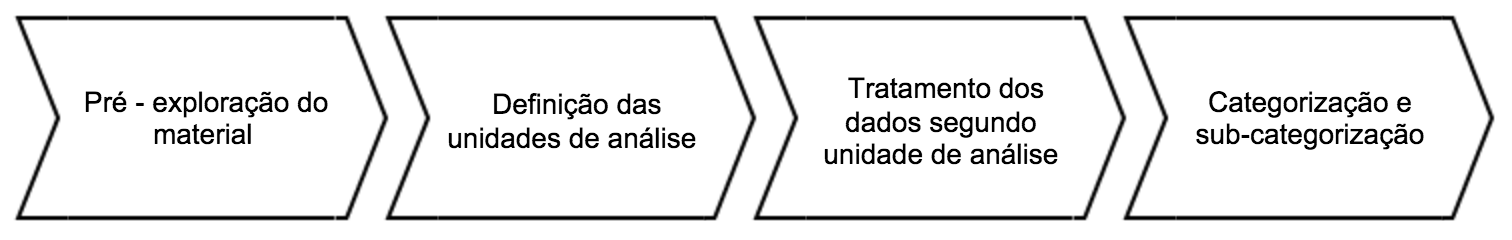
\includegraphics[scale=0.5]{img/fasesanalisedeconteudo}}
\label{fig:fasesanalisedeconteudo}
\caption* {Fonte: Simplificação do modelo \citeonline{bardin} realizada pelo autor}
\end{figure}

A fase inicial de pré-exploração tem como principal objetivo conhecer o contexto do material a ser analisado, retirar impressões e orientações para a próxima etapa. Um dos principais mecanismos dessa etapa é a leitura flutuante, que permite um primeiro contato com o conteúdo do "corpus de análise", raso o suficiente para gerar a formulação de algumas hipóteses e não tomar tempo excessivo do analista. A leitura menos aderente permite a assimilação do "corpus de análise" de forma não-estruturada permitindo a transcendência da mensagem de forma explícita para visualizar pistas não inicialmente óbvias.

Em seguida, é necessário definir a unidade de análise a ser trabalhada, baseada no conteúdo do material avaliado. Essas unidades podem incluir palavras, frases, parágrafos, textos inteiros, de tal forma que possa ser feito algum tipo de análise utilizando-as. A partir das inferências obtidas na etapa anterior, é possível que já tenha sido visualizado que tipo de análise ou categorização poderia ser feito posteriormente, dependendo do tipo de dado analisado. Quando há uma grande repetição de informação devido a um escopo fechado de cada mensagem, é possível utilizar palavras ou frases como unidade de análise para uma posterior análise frequencial. Para os casos em que há uma diversidade maior de informação, a utilização de trechos maiores de texto permitem uma análise temática, a fins de categorização posterior.

Como pode se tratar de um grande volume de dados, é possível que haja a necessidade de um tratamento desses dados de forma a chegar em representações condensadas e explicativas. Para textos maiores, seria oportuno coletar somente as partes relevantes que explicam o conteúdo da própria mensagem passada. Já para palavras e frases, é possível que ocorram palavras sinônimas e frases com o mesmo conteúdo semântico, que tratadas dentro de um mesmo contexto facilitariam a sua categorização posterior. Dentro desse contexto, softwares simples de contagem de palavras até outros mais complexos baseados em algoritmos de \textit{Machine Learning} ganham um espaço de atuação muito grande nessa área, por agilizar esse tipo de tratamento.

Finalmente, através do tratamento desses dados, é possível segmentar as unidades de análise em categorias e em sub-categorias, se necessário. O nível de granularidade ou o gênero dessas categorias deve variar segundo os pontos que querem ser abordados na análise, entretanto recomenda-se fazer a categorização em um nível mais granular, para poder ser feita uma recategorização em níveis menos granulares posteriormente, se necessário.

\subsection{Análise SWOT}
\label{cha:analise_swot}

A análise SWOT é uma ferramenta utilizada para analisar o ambiente e o contexto em que uma empresa se encontra posicionada diante do mercado. O processo de utilização consiste basicamente em organizar características da empresa e do ambiente em que se encontra em quatro principais avaliações: Pontos Fortes (\textit{Strengths}), Pontos Fracos (\textit{Weaknesses}), Oportunidades (\textit{Opportunities}) e Ameaças (\textit{Threats}), conforme quadro ilustrado abaixo. Essa modalidade de análise tem como principal vantagem a simplificação de uma estrutura complexa apresentada por uma organização, facilitando na tomada de decisões estratégicas.

\begin{figure}[H]
\caption{Quadro SWOT básico}
\centerline{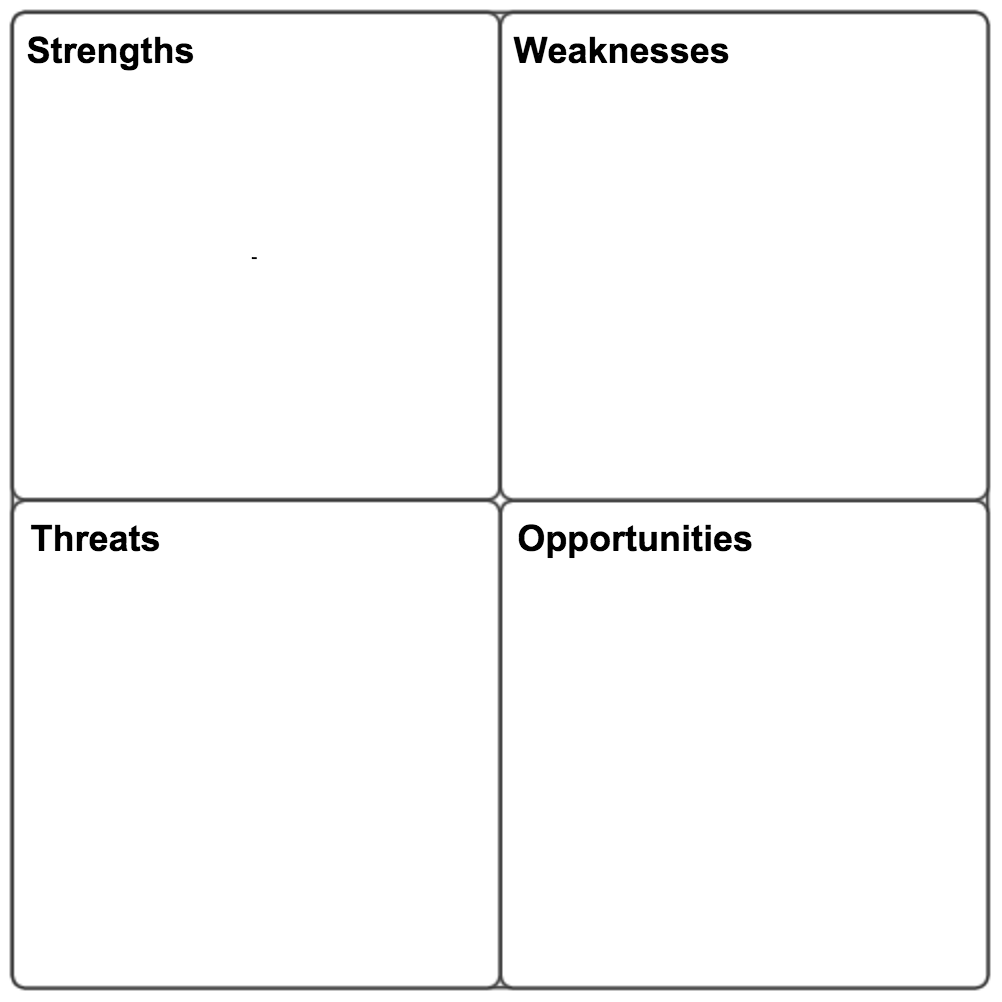
\includegraphics[scale=0.5]{img/detailedswot}}
\label{fig:detailedswot}
\caption* {Fonte: Quadro SWOT básico}
\end{figure}

\section{Método}

\label{chap:metodologia}

\begin{figure}[h]
\caption{Metodologia Utilizada no Trabalho}
\centerline{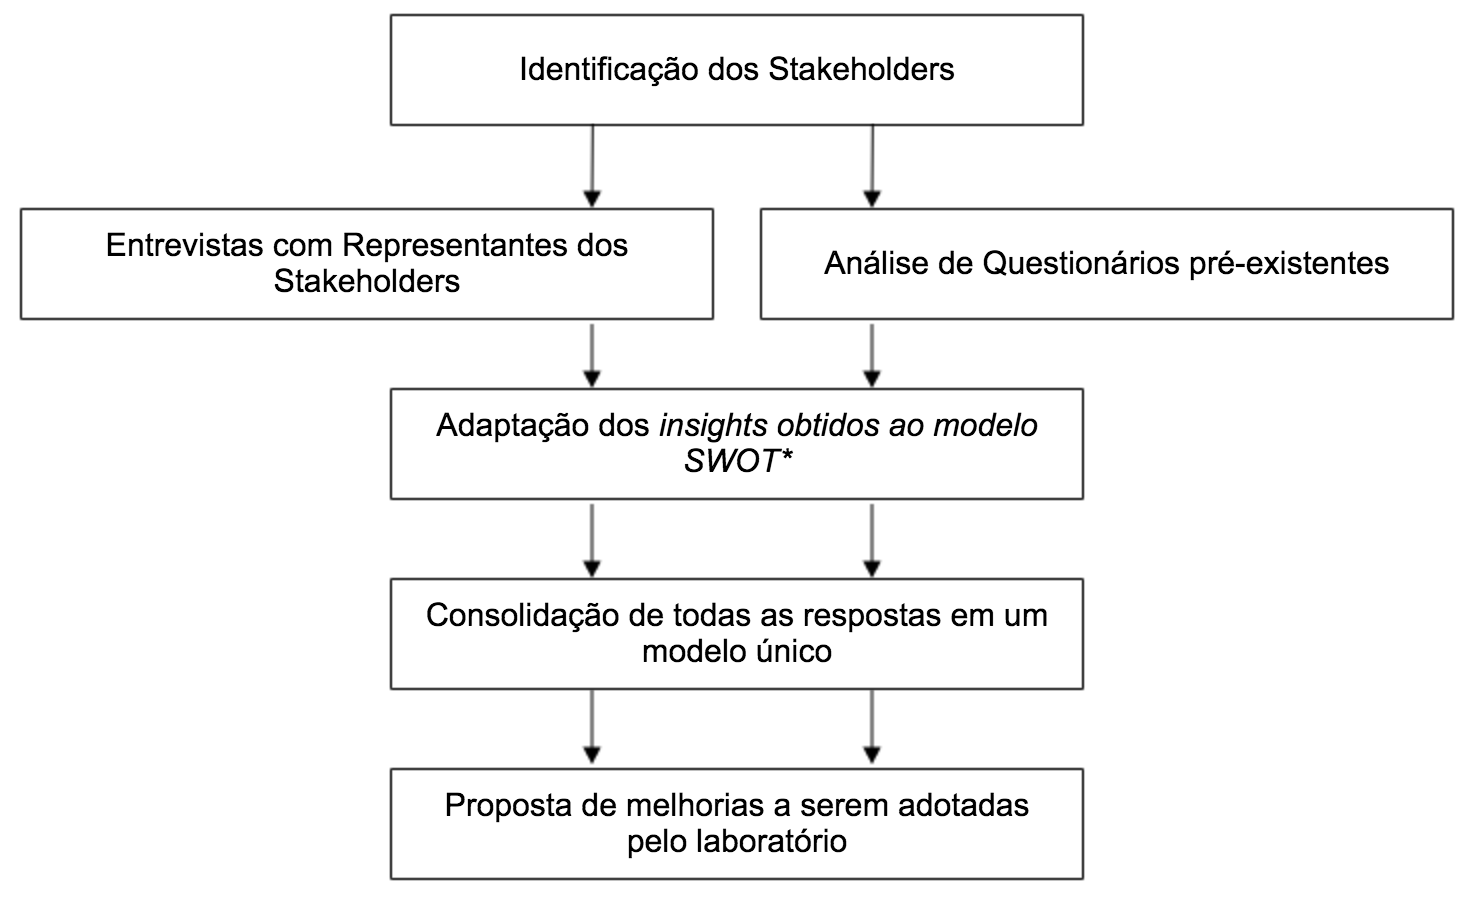
\includegraphics[scale=0.5]{img/metodologia}}
\label{fig:metodologia}
\caption* {Fonte: Elaborado pelo próprio autor}
\end{figure}

Após conversas iniciais com membros da Samsung e do PRO, foram definidos os stakeholders do projeto Ocean, juntamente com as pessoas-chave de cada. Foram realizadas entrevistas semi-estruturadas e gravadas, de forma a permitir a liberdade para serem feitas perguntas não presentes na estrutura inicial, e assim ter uma conversa guiada com o entrevistado como se não fosse uma entrevista formal. Antes de cada entrevista eram preparadas perguntas relacionadas ao mapeamento e percepção das interações do \textit{stakeholder} com o Ocean segundo a visão do entrevistador, e para todos os entrevistados era perguntado "se a pessoa teria alguma sugestão para a melhoria do Laboratório".

Para análise de um \textit{stakeholder} em particular, representado pelo alunos dos cursos básicos do programa Ocean que serão apresentados nesse capítulo, o método de entrevistas foi considerado menos eficiente pelo alto número e rotatividade de alunos. Juntamente a este fato, a Samsung tinha uma necessidade de analisar questionários de \textit{feedback} respondidos nos últimos dois anos de cursos, que nunca haviam sido analisados diante das suas questões qualitativas, apenas das quantitativas. Dessa forma, foram unidas as necessidades de ambas as partes e foram aproveitados esses questionários - totalizando um total de 5280 respostas - para extrair as informações necessárias para este trabalho. O modelo de questionário aplicado encontra-se em anexo. No caso, foram analisadas somente as respostas das questões analíticas: "O que mais o motivou nesse curso?", "O que você acha que pode ser melhorado?" e "Qual tema você gostaria que fosse abordado num próximo curso?".

De forma a analisar e extrair informações desses questionários, o autor optou por desenvolver um software próprio (https://github.com/GabrielArakaki/wordAnalysis) para manipular esses dados via palavras-chave, pelos motivos elencados a seguir.

\begin{description}
\item [Volume de Dados] A quantidade de dados é grande o suficiente para dificultar - porém não inviabilizar - a leitura individual de cada uma das respostas. Acredita-se que mesmo que se optasse pela leitura individual, ela deveria ser acompanhada de uma \textit{clusterização} das respostas em categorias, o que a análise via repetição de palavras-chave também permite encontrar. Em contrapartida, os dados são suficientemente pequenos a ponto de não ser viável buscar alternativas  de \textit{Machine Learning} existentes para tratar esses dados, pois o volume não seria suficiente para treinar a inteligência artificial utilizada.

\item [Proposta do Estudo] Embora exista um campo muito grande de possibilidades de tratar e manipular os dados presentes, existe a necessidade de seguir com os objetivos inicias do presente estudo, que diz respeito ao estudo do projeto Ocean de forma holística, e não somente na questão do aprendizado transmitido através de seus cursos. O autor acredita que há espaço para análises mais sofisticadas - dignas de um trabalho dedicado somente a isso - que poderiam ser realizadas caso a Samsung encontre a necessidade de entender os cursistas nos mínimos detalhes.

\item [Manipulação de Dados] O uso de uma ferramenta própria dá ao autor a liberdade de trabalhar e iterar em cima dos dados de forma a otimizar a ferramenta para o próprio uso. Existem disponíveis ferramentas prontas de geração de nuvens de palavras, que possuem um intuito muito maior de apresentar um 'choque visual' do que apresentar dados analíticos em si. A manipulação de dados permite que o autor encontre associações entre palavras ao observar os dados gerados pela ferramenta e trabalhar em cima da própria ferramenta para eliminar redundâncias ou dados inconsistentes.

\item [Desenvolvimento Ágil] O desenvolvimento ágil é um \textit{framework} de desenvolvimento de software que possui o intuito de permitir o desenvolvimento em um curto período de tempo com um iterações feitas através da coleta de \textit{feedbacks} de forma rápida e sistemática. No caso deste trabalho, o autor não encontrou uma ferramenta que fornecesse customização e flexibilidade conforme suas necessidades, fazendo com que optasse por desenvolver um software próprio. Não obstante, é de satisfação do autor como desenvolvedor utilizar programação para resolver problemas reais.
 
\end{description}

Para consolidar a análise realizada para cada \textit{stakeholder}, foi utilizada uma adaptação do modelo SWOT para ilustrar as percepções obtidas de cada um. Ela difere do modelo original do SWOT por não se tratar de uma análise de negócio baseada em fatores de mercado e competitividade com outros \textit{players}, e sim em uma análise fria e absoluta de fatores básicos em um projeto: Pontos Fortes, Pontos Fracos, Oportunidades e Ameaças. Foi considerado que por ser um modelo simples e de fácil visualização, consolidaria as necessidades deste trabalho sem desvirtuar os objetivos propostos.

A partir dos resultados obtidos pela análise das respostas, trabalhou-se em cima da geração de propostas de melhoria.

\section{Identificação de Stakeholders do Laboratório}
\label{sec:identificacao_stakeholders}

A partir de conversas informais com os professores mais próximos ao projeto Ocean e com os próprios responsáveis da Samsung pelo laboratório, foi possível desenhar um mapa ilustrativo para os principais \textit{stakeholders}.

\begin{figure}[H]
\caption{Mapa de stakeholders do projeto Ocean}
\centerline{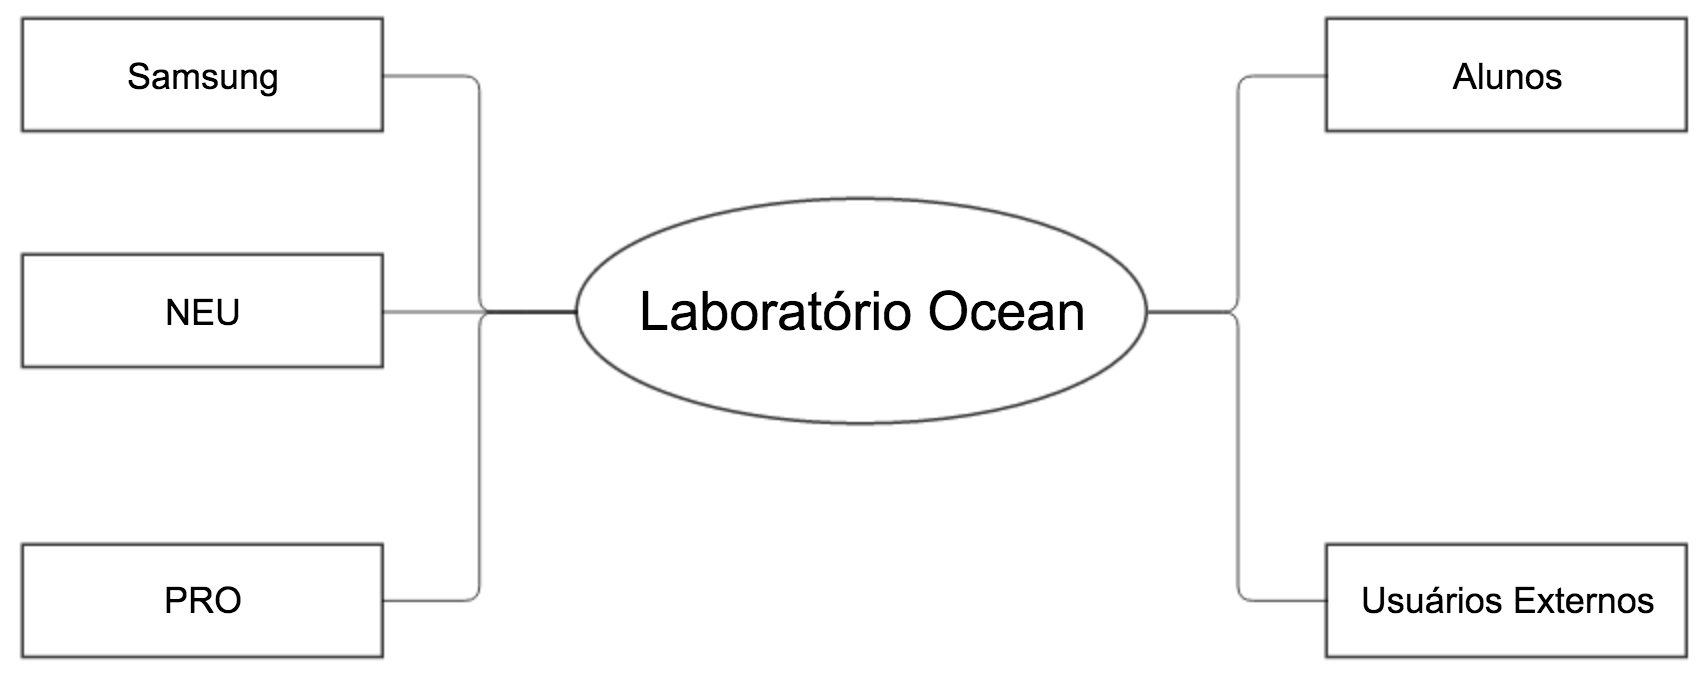
\includegraphics[scale=0.5]{img/stakeholders_v2}}
\label{fig:stakeholders}
\caption* {Fonte: Elaborado pelo próprio autor}
\end{figure}

Em um segundo momento foram definidos as principais fontes de dados para cada um dos \textit{stakeholders}, assim como os principais métodos de coleta, sendo definido o aproveitamento de questionários já respondidos pelos cursistas básicos e entrevistas para os demais.

\begin{figure}[H]
\caption{Pontos de contato dos \textit{stakeholders}}
\centerline{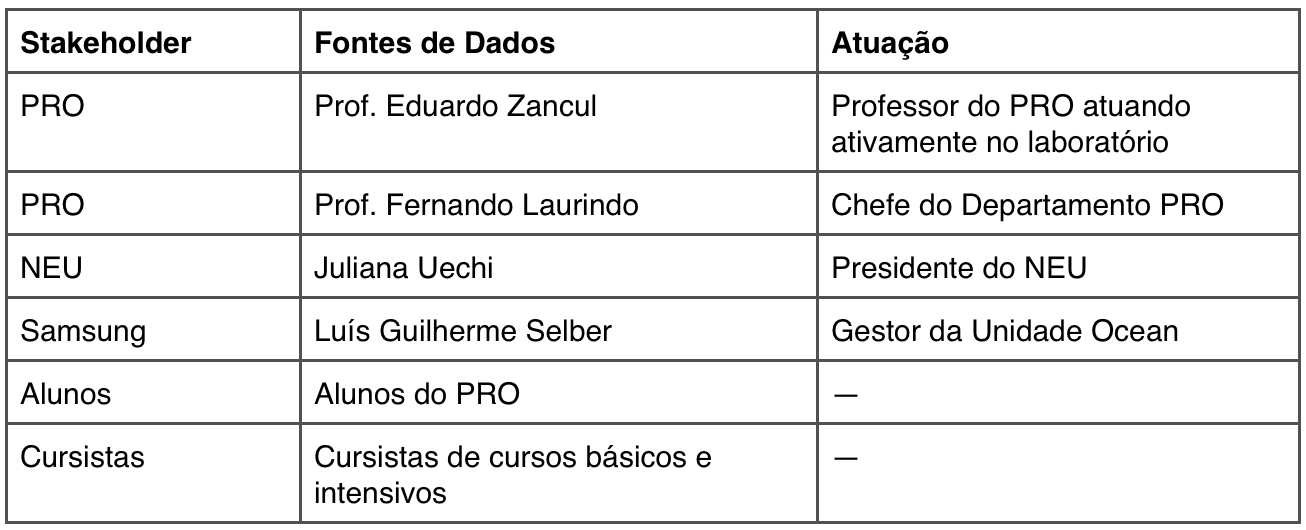
\includegraphics[scale=0.6]{img/stakeholderspoc}}
\label{fig:stakeholderspoc}
\caption* {Fonte: Elaborado pelo próprio autor}
\end{figure}


\subsection{PRO}
\label{sec:con_pro}

O Ocean é um dos quatro grandes projetos que o PRO acompanha atualmente, esquematizado pela Tabela \ref{tab:pilares_pro}, juntamente com Inovalab, a Fábrica Didática e o Núcleo de Empreendedorismo da USP.

\begin{table}[H]
\begin{center}
\caption{Pilares do PRO}
\label{tab:pilares_pro}
{\def\arraystretch{2}\tabcolsep=10pt
\begin{tabular}{>{\raggedright}p{0.2\linewidth}>{\raggedright\arraybackslash}p{0.2\linewidth}>{\raggedright\arraybackslash}p{0.2\linewidth}>{\raggedright\arraybackslash}p{0.2\linewidth}}
\hline
     & Objetivo Institucional & Participação do PRO & Em Atividade  \\ \hline
     Inovalab & Laboratório de Inovação & Gestão Ativa & Sim  \\
     Fábrica Didática & Apropriação de conceitos de fábricas para aplicação no ensino & Em Desenvolvimento & Não \\
     Ocean & Laboratório de Desenvolvimento de Software & Cogestão com a Samsung & Sim \\
	 Núcleo de Empreendedorismo da USP & Disseminação da cultura empreendedora & Cede espaço físico & Sim \\ \hline
\end{tabular}%
}
\caption* {Fonte: Elaborado pelo autor em conversa com professores do departamento}
\end{center}
\end{table}

O Inovalab é um laboratório que oferece recursos para realização de projetos de engenharia, como \textit{software}, \textit{hardware}, impressoras 3D e oficinas mecânicas. A infraestrutura do laboratório é utilizada para sediar o NEU, outro dos projetos que será discutido adiante. Já a Fábrica Didática é um projeto que consiste na produção de peças e produtos com a perspectiva de gerar pesquisa na área de fabricação e ensino para os alunos da engenharia de produção.

O que pode se ver em comum entre esses projetos e o Ocean é a proximidade da inovação e do empreendedorismo, pontos que o PRO considera essenciais para a tríade pesquisa, ensino e extensão. A Engenharia de Produção na Poli propicia um ambiente de aprendizado com disciplinas que já contribuem nessa área, como Projeto Integrado e Desenvolvimento de Produto, porém grande parte do aprendizado pode ser obtido através de atividades extra curriculares, propiciadas em parte por esses projetos. Um dos principais métodos de aprendizagem que a Poli incentiva nos alunos é o \textit{self-learning}, pois a área de Engenharia cobre uma variedade tão extensa de temas que o aluno que tiver interesse em se aprofundar em temas específicos deve buscar conhecimento por conta própria, sendo o principal papel da faculdade fornecer uma base sólida e uma estrutura para que ele possa adquirir conhecimento com facilidade.

\subsection{NEU}
\label{sec:con_neu}

O Núcleo de Empreendedorismo da USP é uma organização formada por alunos de graduação e pós-graduação, pesquisadores e professores que possuem a missão de promover a cultura de empreendedorismo dentro da Universidade. O NEU é aberto à toda comunidade da USP, já tendo recebido contribuições de diversas instituições da universidade, porém é formado atualmente principalmente por alunos da POLI e da FAU.

De forma similar ao estabelecimento do Ocean dentro do departamento do PRO, o NEU foi convidado a utilizar o espaço do Laboratório de Inovação (InovaLab) para sediar suas atividades. Atualmente o NEU trabalha com três principais pilares: inspiração, capacitação e conexão.

Inspiração diz respeito ao fomento ao empreendedorismo nos alunos para que eles se sintam impulsionados a participar do ecossistema de \textit{startups} ou até abrir as suas próprias. Portanto são feitos diversos convites aos diretores de diversas \textit{startups}, muitos com origens da própria USP, como Lean Survey, 99 Táxis e Squid, e estes podem explicar um pouco da sua trajetória e das emoções vividas graças aos seus empreendimentos. 

Capacitação é a frente do NEU de auxiliar ideias de alunos a se desenvolverem em produtos, para que assim sejam criadas novas empresas. A partir da rede de empresas que o NEU tem em seu leque de contatos, ele consegue encontrar mentorias para as empresas e acelerar o seu desenvolvimento. O principal programa dessa frente é o \textit{Startup Lab}, em que o NEU fornece material de apoio e mentoria através dos seus contatos com empresas, investidores e aceleradoras.

Conexão é representado principalmente pelo \textit{Startup Ship}, que é o canal do NEU destinado a alunos que querem estagiar em \textit{startups}. Através de sua rede de conexões ela facilita com que \textit{startups} e os alunos certos cheguem uns aos outros. Outro programa é o Pesquisas USP, que auxilia os alunos a se conectarem com pesquisas, e em contrapartida auxiliar pesquisadores a se conectarem com alunos ou empresas que possam auxiliar nos seus estudos. Nesse programa o NEU também auxilia startups a entrarem em contato com aceleradoras.

O NEU apresenta uma sinergia muito grande com o Ocean, pois ambos possuem muito interesse nessa fase de pré-aceleração de empresas, conseguindo exercer etapas distintas e complementares nesse processo. Durante os cursos intensivos do Ocean, o NEU se responsabiliza por trazer contatos de diferentes empresas para inspirar e fazer mentorias, ao passo que a Samsung trabalha fortemente na parte de capacitação e acompanhamento da evolução das empresas ao longo do programa.

Existe uma série de organismos dentro da universidade que fomentam a cultura de empreendedorismo, e como todos são gratuitos, existe uma colaboração muito grande para que os maiores beneficiados sejam as \textit{startups}, independente de  qual instituição que esteja contribuindo mais para a evolução da empresa.

\subsection{Alunos}
\label{sec:con_alunos}

A Engenharia de Produção é uma área que tem suas origens na engenharia mecânica, pois a formação de engenheiros no passado era voltada principalmente à capacitação técnica de produção de peças e produtos, sem um estudo aprofundado de como fabricá-los com eficiência. Os estudantes eram ensinados a desenhar um produto e desconstruí-lo em diversas peças que deveriam atuar conjuntamente para o funcionamento desejado. Encontrou-se então uma oportunidade de criar um novo ramo da Área Mecânica que se encarregaria de capacitar os alunos a aplicar conceitos de fábrica utilizados globalmente, como otimização das linhas de produção, controle da qualidade e controle da produção, não explorados anteriormente nos cursos de engenharia. Inicialmente voltado principalmente ao setor automotivo, a área de produção começou a ser expandida para poder aplicar os mesmos conceitos de fábrica para qualquer indústria, exigindo uma abstração dos principais conceitos, e inclusive a adoção de teorias de administração e gestão de projetos.

Atualmente, duas disciplinas eletivas estão utilizando a infraestrutura do laboratório, Desenvolvimento Integrado de Produto e Criação de Negócios Tecnológicos, porém o laboratório cede seu espaço a disciplinas que necessitem dos seus recursos. Muitas das reclamações dos alunos em relação ao ensino atual diz respeito às aulas que são passadas utilizando tecnologias antigas, como retroprojetores. Embora o laboratório não esteja sendo usado pelas disciplinas obrigatórios, os alunos enxergam que a sua presença eleva o patamar de tecnologia de ensino a ser utilizado, o que no curto ou médio prazo pode abandonar as tecnologias antigas para adotar o maior uso de mídias digitais.

Além da questão das disciplinas, o laboratório é utilizado pelos alunos durante o período fora da aula, para a realização de trabalhos , tarefas ou para fixar o conteúdo que foi dado em aula. Como o laboratório fica aberto até as 22 horas, e na cultura da engenharia é bastante comum ficar até tarde estudando, alunos utilizam o laboratório praticamente o dia inteiro. Antes do laboratório era frequente os alunos irem estudar em outros departamentos como a Engenharia Civil, que possui várias mesas no seu saguão principal, e ficava aberta até tarde para os alunos de pós-graduação. Embora grande parte dos alunos traz o seu próprio \textit{notebook} para estudar, alguns utilizam os notebooks da própria samsung e até um outro monitor para otimizar as suas tarefas.

A presença de um laboratório como este também ajuda a fomentar a cultura de empreendedorismo dentro da universidade, pois permite a capacitação dos alunos diante do desenvolvimento de produtos, base de criação de novas \textit{startups}. Segundo as pesquisas realizadas por \citeonline{entrepreneurship} com estudantes de graduação de engenharia, a experiência de empreendedorismo é observado de 4 maneiras, independentemente se eles desejam empreender ou não: 

\begin{enumerate}
\item Primeiro passo para o auto-aprendizado
\item Preparação para a vida no trabalho
\item Caminho para ser autônomo
\item Desenvolvimento de liderança e responsabilidade de um time
\end{enumerate}

Como esses pontos seguem na mesma direção dos objetivos da Poli e não agrada somente aqueles alunos que desejam ser empreendedores, o PRO pode continuar fomentando o empreendedorismo para que atinja todos os alunos. Entretanto, de forma a potencializar ainda mais os futuros empreendedores, é necessário entender o perfil daqueles alunos que desejam abrir o seu próprio negócio, como foi observado em diversas pesquisas como a realizada por \citeonline{empreendedorismo}, em que identifica o perfil de alunos que são atraídos pelo empreendedorismo:

\begin{itemize}
\item Propensão a assumir riscos
\item Proximidade a outros empreendedores no círculo próximo
\item Já possuem uma ideia desenvolvida para o empreendimento
\end{itemize}


\subsection{Cursistas}
\label{sec:con_cursistas}

Conforme explicado anteriormente, o Ocean trabalha com duas propostas de cursos, os cursos básicos e os cursos intensivos. O primeiro grupo corresponde à capacitação de desenvolvedores para que gerem conteúdo através de \textit{software} para dispositivos da Samsung, já o segundo é para pessoas que desejam empreender e possuem uma ideia inicial para ser desenvolvida. Embora exista uma gama de pessoas que seja usuária de ambos os cursos - os novos empreendedores têm muito interesse por programação - o público-alvo de cada um é diferente.

Os cursos básicos são desenhados para programadores ou aspirantes à programação. Embora existam diversos temas de cursos, o principal objetivo da Samsung consiste em capacitar os cursistas a explorarem todas as funcionalidades permitidas pelos \textit{hardwares} da Samsung. Para isso, são explorados o sistema operacional Android, os SDKs da Samsung, o sistema operacional Tizen, em suma tudo que possa contribuir para que o desenvolvedor possa gerar valor e conteúdo sem se preocupar em desenvolver um hardware específico. Portanto, é um curso de bastante interesse para iniciantes que desejam iniciar o aprendizado em programação, para desenvolvedores experientes que não tiveram muito contato com dispositivos móveis até para apaixonados pela Samsung que querem verificar na prática todo potencial permitido pelos seus dispositivos.

Segundo a 27\textsuperscript{a} Pesquisa de Anual do uso de TI, realizada pela Fundação Getúlio Vargas (FGV), o número de smartphones em uso no Brasil gira atualmente em torno de 168 milhões de dispositivos. \cite{tifgv}. Não obstante, além do alto número de smartphones, o Brasil também se mostra presente no mercado de outros dispositivos inteligentes, com previsão de movimentação de US\$4,1 bilhões no Brasil com IOT, segundo a assessoria de imprensa da IDC Brasil. \cite{idc}. Segundo a ONG Code.org, financiada por fundadores das maiores empresas de tecnologia do mundo como Mark Zuckerberg e Bill Gates, o número de empregos para programadores cresce exponencialmente, ao passo que o ensino de programação nas escolas não acompanha o mesmo ritmo, o que gerará uma falta de profissionais de TI em um futuro próximo. Juntamente a essa informação, o departamento de estatísticas de trabalho dos Estados Unidos (\textit{Bureau of Labor Statistics}) estima que o número de empregos para programadores fora dos EUA para trabalho remoto aumentará consideravelmente. \cite{bls}

É nesse cenário de alto crescimento do uso de novas tecnologias no Brasil que o mesmo se mostra como um grande mercado para produtos inerentes ao uso de dispositivos inteligentes, como aplicativos e games. Dentro desse contexto, jovens interessados pelo desenvolvimento desse mercado no país se interessam por propostas como a do Ocean para realizar diferentes cursos nessas áreas.
 
O segundo tipo de curso - cursos intensivos - foram feitos para incentivar ideias a se tornarem empresas, então é voltado para o nicho empreendedor. De acordo com o projeto \textit{Global Entrepreneurship Monitor}, que realiza pesquisas anuais sobre empreendedorismo no mundo, estima-se que em 2015, 52 milhões de brasileiros com idade entre 18 e 64 anos se envolveram na criação ou manutenção de algum negócio. Entre 2015 e 2014, houve um salto do total de empreendedores entre pessoas de 34,4\% para 39,9\% da população da faixa etária mencionada, principalmente devido ao surgimento de novas empresas. \cite{GEM}

Uma pequena parte dessas empresas é constituída de empresas com alto valor agregado e/ou com produtos de alta tecnologia, porém é visível o aumento da procura de pessoas que possuem ideias e buscam algum tipo de mentoria para desenvolvê-las a ponto de poder empreender. É nesse momento em que elas encontram o Ocean, onde podem utilizar de toda \textit{expertise} da Samsung para desenvolver um produto ou serviço de alta qualidade. Portanto não é necessário que os grupos já possuam uma empresa e um produto em funcionamento, até porque o programa desses cursos envolve questionar e validar hipóteses a respeito do próprio modelo de negócio da empresa, independente da maturidade da ideia. 

Os cursos intensivos são de uma extensão muito maior, e exigem uma intensidade muito grande dos cursistas, com reuniões de três horas de segunda à quinta-feira. Esse fator mostra a seriedade do programa em trabalhar com pessoas que mostrem um comprometimento acima da média, até porque muitos dos cursistas possuem emprego fixo e devem arranjar um tempo para se dedicar ao programa. Não obstante, além de ter esse acompanhamento quase diário nos dias úteis, são definidas metas semanais a serem cumpridas, para guiar as equipes no seu planejamento da semana. Toda essa intensidade tem o objetivo de deixar os alunos engajados ao longo do curso, que por ser gratuito e não exigir participação societária por parte da Samsung, pode facilmente ser abandonado se o aluno não observar o comprometimento da própria empresa.
%%!TEX root = index.tex
\section[Requisitos]{Requisitos}
\begin{frame}{Requisitos}

\begin{itemize}
	\item $20\%$ Precisão
	\item $20\%$ Abrangência
\end{itemize}

\begin{table}[htp]
\begin{center}
    \caption{Avaliação de sistemas de predição}
    \vspace{-.5cm}
    \label{tab:avaliacao-predicao}
    \begin{tabular}{  | c | c | p{4cm} | }
    \hline
    \textbf{Medida} & \textbf{Fórmula} & \textbf{Significado} \\ \hline
    Precisão &  $\frac{VP}{VP+FP}$ & Porcentagem de casos positivos corretamente preditos. \\ \hline                            
    Abrangência & $\frac{VP}{VP+FN}$ & Porcentagem de casos positivos sobre aqueles que foram marcados como positivos. \\ \hline
    $F_1$ &  $2 \cdot \frac{\mathrm{Precisão}~\cdot~\mathrm{Abrangência}}{\mathrm{Precisão}~+~\mathrm{Abrangência}}$ & Média harmônica entre precisão e abrangência. \\ \hline
    \end{tabular}
\end{center}
\end{table}

\end{frame}

%\begin{block}{Requisitos não funcionais}
%\begin{itemize}
%	\item Escalabilidade
%	\item Sistema genérico
%	\begin{itemize}
%		\item Padronização dos dados de entrada/saída
%	\end{itemize}
%	\item Código aberto
%\end{itemize}
%\end{block}
%\end{frame}

%\begin{frame}{Requisitos}{Diagrama de Casos de Uso}
%\begin{columns}[c]
%\column{.6\textwidth}
%\textbf{Três principais grupos}
%	\begin{itemize}
%		\item Avaliar Performance
%		\item Configurar Banco de Dados
%		\item Recomendar
%	\end{itemize}
%\column{.45\textwidth}
%\begin{figure}[ht]
%    \begin{center}
%    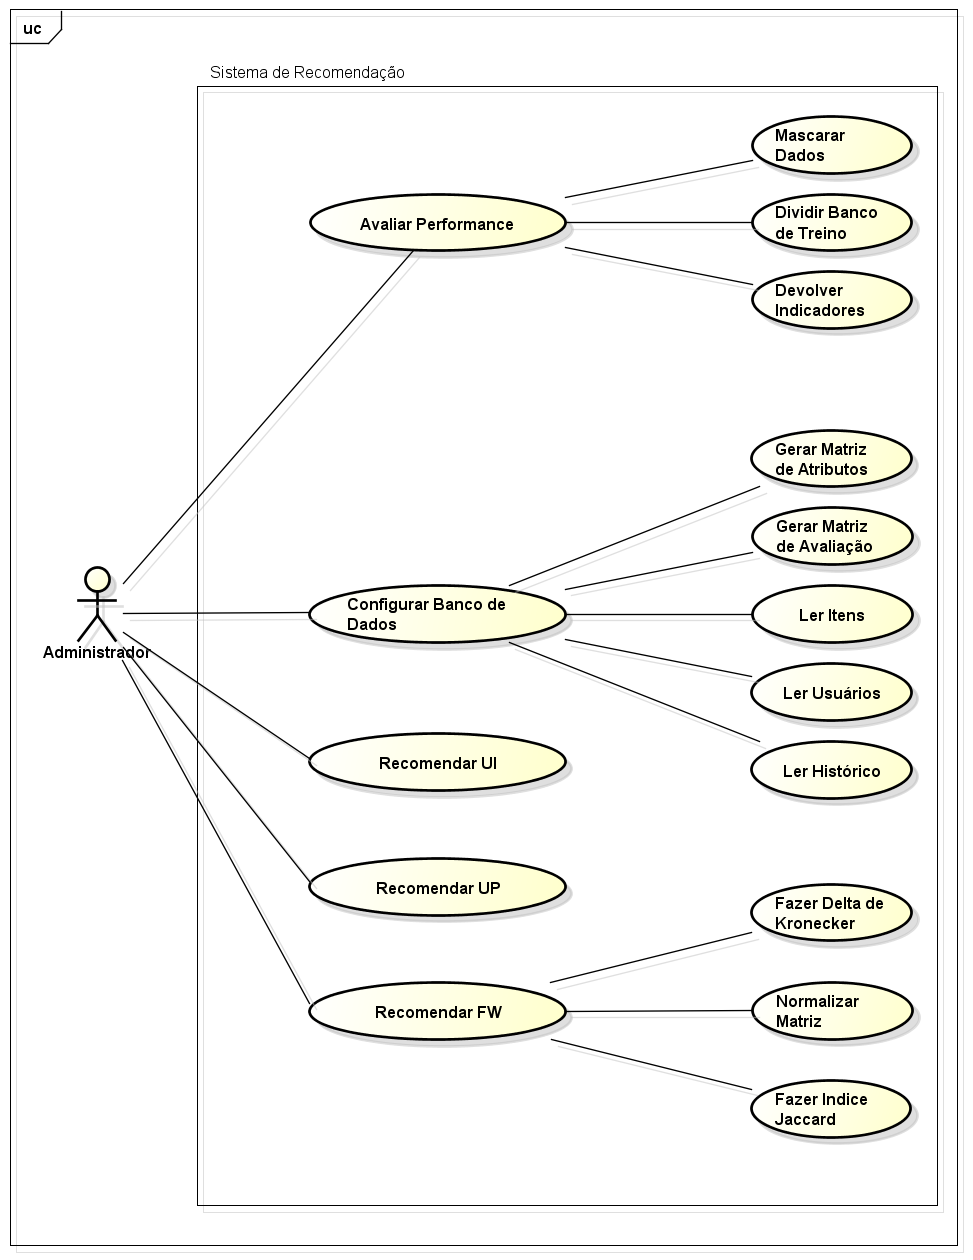
\includegraphics[width=0.9\textwidth]{img/CasosDeUso}
%    \end{center}
%\caption{Diagrama de Casos de Uso}
%\end{figure}
%\end{columns}
%\end{frame}
%
%
%\begin{frame}{Requisitos}{Diagrama de Casos de Uso - Avaliar Performance}
%
%\begin{figure}[ht]
%    \begin{center}
%    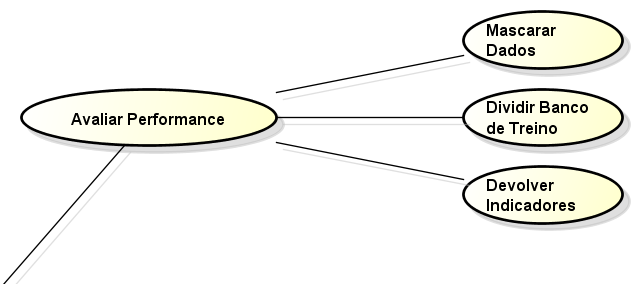
\includegraphics[width=0.9\textwidth]{img/CasosDeUso_Avaliar_Performance}
%    \end{center}
%\caption{Caso de Uso - Avaliar Performance}
%\end{figure}
%\end{frame}
%
%\begin{frame}{Requisitos}{Diagrama de Casos de Uso - Configurar Banco de Dados}
%
%\begin{figure}[ht]
%    \begin{center}
%    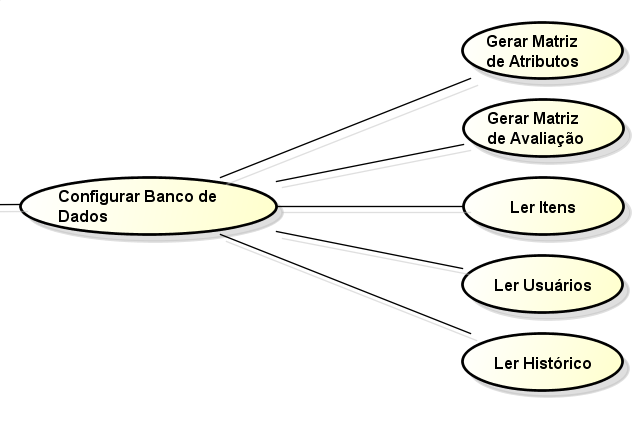
\includegraphics[width=0.9\textwidth]{img/CasosDeUso_Configurar_banco}
%    \end{center}
%\caption{Caso de Uso - Avaliar Performance}
%\end{figure}
%\end{frame}
%
%\begin{frame}{Requisitos}{Diagrama de Casos de Uso - Recomendar}
%
%\begin{figure}[ht]
%    \begin{center}
%    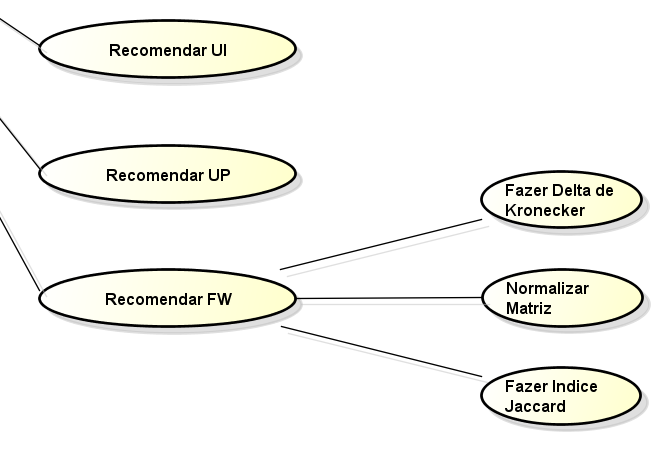
\includegraphics[width=0.9\textwidth]{img/CasosDeUso_Recomendar}
%    \end{center}
%\caption{Caso de Uso - Recomendar}
%\end{figure}
%\end{frame}
%!TEX root = index.tex
\section{Avaliação de Desempenho} % (fold)
\label{cha:avalia_o_de_desempenho}

% chapter avalia_o_de_desempenho (end)

% chapter avalia_o_do_sistema_de_recomenda_o (end)

% section avalia_o_do_sistema_de_recomenda_o (end)

De modo geral, sistemas de recomendação tem o objetivo de apresentar ao usuário itens pelos quais ele possa se interessar. O desempenho de um sistema de recomendação se mede, portanto, na qualidade com a qual ele executa essa tarefa. 

Essa qualidade pode ser medida de diferentes maneiras, tal como pela medida de distância entre os produtos recomendados $\hat{\textbf{\i}}$ e aqueles que seriam efetivamente comprados $\textbf{i}$ pelo cliente em uma validação cruzada (\textit{cross validation}). Outras medidas de predição também podem ser utilizadas, a exemplo de trabalhos de recuperação de informação, tais como acurácia (\textit{accuracy}), especificidade (\textit{specificity}), precisão (\textit{precision}), abrangência (\textit{recall}), medida $F_1$ (\textit{$F_1$-score}), e outras \cite{herlocker2004evaluating}. 

No nosso Trabalho de Conclusão de Curso, serão utilizados precisão, abrangência, e medida $F_1$. Essas medidas foram escolhidas a fim de se poder estabelecer uma base comparativa com os textos de referência, que também as utilizam, e com  algoritmos que fornecem recomendações do tipo lista \textit{top-N}  \cite{cremonesi2010performance}. As medidas estão sumarizadas na Tabela \ref{tab:avaliacao-predicao}. As quantidades $VP$, $FP$, $VN$ e $FN$ significam o número de verdadeiro e falso positivos e o número de verdadeiro e falso negativos.

%\begin{table}[H]
%\begin{center}
%    \caption{Matriz de confusão}
%    \label{tab:avaliacao-predicao}
%    \begin{tabular}{ | l | l | p{5cm} | p{5cm} | }
%    \hline
%    & & \multicolumn{2}{|c|}{Caso predito} \\ \hline 
%    & & \textbf{Positivo} & \textbf{Negativo} \\ \hline
%    \multirow{2}{*}{Caso real} 
%        & Positivo & Verdadeiro Positivo &  $(VP)$ & Falso Negativo $(FN)$ \\ \hline
%        & Negativo & Falso Positivo $(FP)$ & Verdadeiro Negativo $(VN)$ \\ \hline
%    \end{tabular}
%\end{center}
%\end{table}


%\begin{tabular}{cc|c|c|c|c|l}
%\cline{3-4}
%& & \multicolumn{2}{ c| }{Caso predito} \\ \cline{3-4}
%& & 2 & 3  \\ \cline{1-4}
%\multicolumn{1}{ |c| }{\multirow{2}{*}{Powers} } &
%\multicolumn{1}{ |c| }{504} & 3 & 2 &      \\ \cline{2-4}
%\multicolumn{1}{ |c  }{}                        &
%\multicolumn{1}{ |c| }{540} & 2 & 3 &      \\ \cline{1-4}
%\multicolumn{1}{ |c  }{\multirow{2}{*}{Powers} } &
%\multicolumn{1}{ |c| }{gcd} & 2 & 2   \\ \cline{2-4}
%\multicolumn{1}{ |c  }{}                        &
%\multicolumn{1}{ |c| }{lcm} & 3 & 3   \\ \cline{1-4}
%\end{tabular}


\begin{table}[htp]
\begin{center}
    \caption{Avaliação de sistemas de predição}
    \label{tab:avaliacao-predicao}
    \begin{tabular}{  | >{\arraybackslash} m{3cm} | >{\centering\arraybackslash} m{4cm} | >{\arraybackslash} m{6cm} | }
    \hline
    \textbf{Medida} & \textbf{Fórmula} & \textbf{Significado} \\ \hline
    Precisão &  $\frac{VP}{VP+FP}$ & Porcentagem de casos positivos corretamente preditos. \\ \hline                            
    Abrangência & $\frac{VP}{VP+FN}$ & Porcentagem de casos positivos sobre aqueles que foram marcados como positivos. \\ \hline
%    Especificidade & $\frac{VN}{VN+FP}$ &  Porcentagem de casos negativos sobre aqueles que foram marcados como negativos. \\ \hline
%    Acurácia & $\frac{VP+VN}{VP+VN+FP+FN}$ & Porcentagem de predições corretas. \\ \hline
    $F_1$ &  $2 \cdot \frac{\mathrm{Precisão}~\cdot~\mathrm{Abrangência}}{\mathrm{Precisão}~+~\mathrm{Abrangência}}$ & Média harmônica entre precisão e abrangência. \\ \hline
    \end{tabular}
\end{center}
\end{table}

Por fim, avaliaremos o desempenho do sistema mediante a mudança nas variáveis de importância do problema, como por exemplo na quantidade de atributos utilizados na recomendação. O tempo de execução também será avaliado em função do algoritmo utilizado e do tamanho do banco de dados.

%e na capacidade de lidar com problemas como o \textit{cold start}
%%!TEX root = index.tex
\chapter[Detalhamento de Soluções]{Detalhamento de Soluções}
\label{chap:sintese_de_solucoes}

A fim de facilitar a compreensão dos métodos propostos neste trabalho, serão utilizadas as matrizes de avaliações $\mathbf{R}$ e de atributos $\mathbf{A}$ abaixo, adaptadas da Referência \citeonline{debnath2008feature}. Em todos os exemplos, considera-se valor mínimo $M=2$. Os logaritmos são expressos em base 10 e todos os pesos $w_f$, descritos a seguir, são utilizados.

\begin{table}[h]
\begin{center}
    \caption{Avaliações $r_{ui}$}
    \label{tab:rui_ref}
    \begin{tabular}{ | c | c | c | c | c | c | c | } 
    \hline
     & $i_1$ & $i_2$ & $i_3$ & $i_4$ & $i_5$ & $i_6$ \\ \hline
     $u_1$ & - & 4 & - & - & 5 & - \\ \hline
     $u_2$ & - & 3 & - & 4 & - & - \\ \hline
     $u_3$ & - & - & - & - & - & 4 \\ \hline
     $u_4$ & 5 & - & 3 & - & - & - \\ \hline
    \end{tabular}
\end{center}
\end{table}

\begin{table}[h]
\begin{center}
    \caption{Atributos $a_{if}$}
    \label{tab:aif_ref}
    \begin{tabular}{ | c | c | c | c | c | } 
    \hline
     & $f_1$ & $f_2$ & $f_3$ & $f_4$  \\ \hline
     $i_1$ & 0 & 1 & 0 & 0  \\ \hline
     $i_2$ & 1 & 1 & 0 & 0  \\ \hline
     $i_3$ & 0 & 1 & 1 & 0  \\ \hline
     $i_4$ & 0 & 1 & 0 & 0  \\ \hline
     $i_5$ & 1 & 1 & 1 & 0  \\ \hline
     $i_6$ & 0 & 0 & 0 & 1  \\ \hline
    \end{tabular}
\end{center}
\end{table}

\section{Algoritmo baseado na ponderação de atributos (FW)} % (fold)
\label{sec:algoritmo_baseado_na_pondera_o_de_atributos_}

% section algoritmo_baseado_na_pondera_o_de_atributos_ (end)

O primeiro algoritmo que utilizaremos no sistema de recomendação, adaptado da Referência \citeonline{symeonidis2007feature} e denominado ponderação de atributos, \textit{feature weighting} ou FW, trata-se de um híbrido entre filtragem colaborativa e filtragem baseada em conteúdo. A partir da regressão linear de dados de uma rede social (\textit{Internet Movie Database, IMDB}), extraem-se os pesos que determinam a importância de cada atributo dos itens, e é onde ocorre a filtragem colaborativa dos usuários. Após obtenção dos pesos, realiza-se a filtragem baseada em conteúdo para determinar os itens com maior similaridade, que são finalmente recomendados.

Na filtragem baseada em conteúdo, ``cada item é representado por um vetor de atributos ou \textit{features}''. A similaridade $s_{ij}$ entre dois itens $i$ e $j$ é dada pela média ponderada das distâncias entre as \textit{features} dos itens:

\begin{equation} 
\label{eq:sij}
    s_{ij} = \sum_{f}{w_{f} \left(1-d_{fij}\right)}
\end{equation}

As distâncias entre os atributos $d_f$ são determinadas conforme o tipo de dado avaliado e seu domínio, normalizadas no intervalo $\left[0,1\right]$. 

Para atributos literais, como categoria, marca, cor, etc., uma possível medida de distância é o delta de Kronecker descrito em \ref{eq:delta}. A similaridade entre as cores ``azul'' e ``vermelho'' é, nesse caso, 0, e sua distância é 1. O valor da distância é nulo se e somente se os atributos são idênticos.

Para atributos pertencentes a uma coleção finita de itens, tais como os atores participantes de um filme, é possível estabelecer a similaridade entre dois conjuntos a partir do índice Jaccard, descrito em \ref{eq:jaccard}. Neste caso, a similaridade entre os conjuntos \{Al Pacino, Tom Hanks\} e \{Tom Hanks, Marlon Brando\} é $1/3$, e a sua distância é $2/3$.


\begin{equation}
\label{eq:delta}
\delta_{mn} =  
\begin{cases}
1, &\text{se }m=n \\
0, &\text{se }m \neq n
\end{cases} 
\end{equation}

\begin{equation}
\label{eq:jaccard}
J(A,B) ={{|A \cap B|}\over{|A \cup B|}}
\end{equation}

Vale considerar a correlação entre atributos no cálculo das distâncias: a similaridade de duas marcas de calçado, por exemplo, é maior que a de duas marcas de produtos de categorias diferentes, mesmo que as marcas sejam distintas nos dois casos. Em uma primeira análise, todavia, utilizaremos para a maior parte das \textit{features} as medidas de distância do delta de Kronecker \ref{eq:dfij_delta} (Tabela \ref{tab:d_ijf}) e do índice Jaccard \ref{eq:dfij_jaccard}. Isso significa que se os atributos de dois itens são idênticos, a distância é nula e portanto a similaridade é máxima. O sumário de algumas medidas de distância que podem ser utilizadas para casos específicos estão na Tabela \ref{tab:medidas-distancia}.

\begin{equation}
\label{eq:dfij_delta}
\begin{split}
d_{fij} =&~ 1-\delta_{ij}^f \\
    =&~ 1-\delta_{a_{if} a_{jf}}
\end{split} 
\end{equation}


\begin{table}[p]
\begin{center}
    \caption{$d_{ij}^{f}$}
    \label{tab:d_ijf}
    \begin{tabular}{ | c | c | c | c | c | c | c | } 
    \hline
     $f_1$ & $i_1$ & $i_2$ & $i_3$ & $i_4$ & $i_5$ & $i_6$  \\ \hline
     $i_1$ & -  &  0  &  1  &  1  &  0  &  1 \\ \hline
     $i_2$ & 0  &  -  &  0  &  0  &  1  &  0  \\ \hline
     $i_3$ & 1  &  0  &  -  &  1  &  0  &  1 \\ \hline
     $i_4$ & 1  &  0  &  1  &  -  &  0  &  1 \\ \hline
     $i_5$ & 0  &  1  &  0  &  0  &  -  &  0 \\ \hline
     $i_6$ & 1  &  0  &  1  &  1  &  0  &  - \\ \hline
    \end{tabular}
    \quad
    \begin{tabular}{ | c | c | c | c | c | c | c | } 
    \hline
     $f_2$ & $i_1$ & $i_2$ & $i_3$ & $i_4$ & $i_5$ & $i_6$  \\ \hline
     $i_1$ & -  &  1  &  1   & 1  &  1  &  0 \\ \hline
     $i_2$ & 1  &  -  &  1   & 1  &  1  &  0  \\ \hline
     $i_3$ & 1  &  1  &  -   & 1  &  1  &  0 \\ \hline
     $i_4$ & 1  &  1  &  1   & -  &  1  &  0 \\ \hline
     $i_5$ & 1  &  1  &  1   & 1  &  -  &  0 \\ \hline
     $i_6$ & 0  &  0  &  0   & 0  &  0  &  - \\ \hline
    \end{tabular}
    
    \begin{tabular}{ | c | c | c | c | c | c | c | } 
    \hline
     $f_3$ & $i_1$ & $i_2$ & $i_3$ & $i_4$ & $i_5$ & $i_6$  \\ \hline
     $i_1$ & -  &  1  &  0  &  1  &  0  &  1 \\ \hline
     $i_2$ & 1  &  -  &  0  &  1  &  0  &  1  \\ \hline
     $i_3$ & 0  &  0  &  -  &  0  &  1  &  0 \\ \hline
     $i_4$ & 1  &  1  &  0  &  -  &  0  &  1 \\ \hline
     $i_5$ & 0  &  0  &  1  &  0  &  -  &  0 \\ \hline
     $i_6$ & 1  &  1  &  0  &  1  &  0  &  - \\ \hline
    \end{tabular}    
    \quad
    \begin{tabular}{ | c | c | c | c | c | c | c | } 
    \hline
     $f_4$ & $i_1$ & $i_2$ & $i_3$ & $i_4$ & $i_5$ & $i_6$  \\ \hline
     $i_1$ & -  &  1  &  1 &   1 &   1  &  0 \\ \hline
     $i_2$ & 1  &  -  &  1 &   1 &   1  &  0  \\ \hline
     $i_3$ & 1  &  1  &  - &   1 &   1  &  0 \\ \hline
     $i_4$ & 1  &  1  &  1 &   - &   1  &  0 \\ \hline
     $i_5$ & 1  &  1  &  1 &   1 &   -  &  0 \\ \hline
     $i_6$ & 0  &  0  &  0 &   0 &   0  &  - \\ \hline
    \end{tabular}        
\end{center}
\end{table}


\begin{equation}
\label{eq:dfij_jaccard}
\begin{split}
d_{fij} =&~ 1-J^f(i,j) \\
    =&~ 1-J(a_{if},a_{jf})
\end{split} 
\end{equation}

\begin{table}[hp]
\begin{center}
    \caption{Medidas de distância entre alguns atributos}
    \label{tab:medidas-distancia}
    \begin{tabular}{  | >{\arraybackslash} m{3cm} | >{\arraybackslash} m{3cm} | >{\centering\arraybackslash} m{3cm} | } 
    \hline
    \textbf{Atributo} $f$ & \textbf{Domínio} $\mathrm{F}$ & \textbf{Distância} $d_f$ \\ \hline
    Marca & Literal & $1-\delta^f_{ij}$ \\ \hline    
    Esporte & Literal & $1-\delta^f_{ij}$ \\ \hline
    Gênero & Literal & $1-\delta^f_{ij}$ \\ \hline            
    Categoria & Conjunto Literal & $1-J^f(i,j)$ \\ \hline            
    Preço & $\mathbb{R}$ & $ \frac{\left| a_{if}-a_{jf} \right|}{\max_{i,j}{\left| a_{if}-a_{jf} \right|}} $ \\ \hline
    Data & $\mathbb{R}$ milissegundos a partir de \textit{epoch} \cite{epoch} & $ \frac{\left| a_{if}-a_{jf} \right|}{\max_{i,j}{\left| a_{if}-a_{jf} \right|}} $ \\ \hline
    \end{tabular}
\end{center}
\end{table}
 
Os pesos $w_f$ são a priori desconhecidos. A Referência \citeonline{symeonidis2007feature} os determina a partir de uma regressão linear do tipo \ref{eq:regressao-linear}, onde $e_{ij}$ é o número de usuários que se interessam tanto por $i$ quanto por $j$. Esses valores permitem determinar ``o julgamento humano de similaridade entre itens'', e pode ser calculado a partir da matriz de avaliações, conforme a equação \ref{eq:determinacao-eij} (Tabela \ref{tab:eij}). O operador booleano $\mathrm{b}_M$, descrito pela Equação \ref{eq:b0}, nada mais é que uma ferramenta matemática para se poder extrair o número de usuários que avaliaram \textit{positivamente} tanto $i$ quanto $j$ a partir de $\mathbf{R}$. 


\begin{equation}
\label{eq:regressao-linear} 
    e_{ij} = w_0 + \sum_{f}{w_{f} \left(1-d_{fij}\right)}
\end{equation} 


\begin{equation}
\label{eq:determinacao-eij} 
    e_{ij} = \sum_{u}{\mathrm{b_M}\left(r_{ui} ~ r_{uj}\right)}
\end{equation} 

\begin{equation}
\label{eq:b0}
\mathrm{b}_M\left(x\right) = 
\begin{cases}
1, &\text{se }x>M \\
0, &\text{se }x\leq M
\end{cases} 
\end{equation}

\begin{table}[p]
\begin{center}
    \caption{$e_{ij}$}
    \label{tab:eij}
    \begin{tabular}{ | c | c | c | c | c | c | c | } 
    \hline
     & $i_1$ & $i_2$ & $i_3$ & $i_4$ & $i_5$ & $i_6$  \\ \hline
     $i_1$ & - & 0 & 1 & 0 & 0 & 0 \\ \hline
     $i_2$ & 0 & - & 0 & 1 & 1 & 0  \\ \hline
     $i_3$ & 1 & 0 & - & 0 & 0 & 0 \\ \hline
     $i_4$ & 0 & 1 & 0 & - & 0 & 0 \\ \hline
     $i_5$ & 0 & 1 & 0 & 0 & - & 0 \\ \hline
     $i_6$ & 0 & 0 & 0 & 0 & 0 & - \\ \hline
    \end{tabular}
\end{center}
\end{table}

Desta forma, os pesos $w_f$ são determinados a partir resolução do sistema de equações lineares \ref{eq:determinacao-wf} (Tabela \ref{tab:w_f}). Apenas os pesos positivos e com valor absoluto expressivo (maior que um piso arbitrariamente escolhido a posteriori) são utilizados na recomendação. 

\begin{equation}
\label{eq:determinacao-wf} 
    w_0 + \sum_{f}{w_{f}  \left(1-d_{fij}\right)} = \sum_{u}{\mathrm{b_0}\left(r_{ui} ~ r_{uj}\right)},~\forall i \neq j 
\end{equation} 

\begin{table}[p]
\begin{center}
    \caption{$w_f$}
    \label{tab:w_f}
    \begin{tabular}{ | c | c | c | c | c | } 
    \hline
     $w_0$ & $w_1$ & $w_2$ & $w_3$ & $w_4$   \\ \hline
     0.41 & -0.22 & -0.34 & -0.03 & -   \\ \hline
    \end{tabular}
\end{center}
\end{table}

Calcula-se a matriz de similaridade $\mathbf{S}$ pela Equação \ref{eq:sij} (Tabela \ref{tab:sij}) e recomendam-se os itens similares àqueles já comprados, segundo \ref{eq:ifw} (Tabela \ref{tab:i_u_fw}).

\begin{table}[p]
\begin{center}
    \caption{$s_{ij}$}
    \label{tab:sij}
    \begin{tabular}{ | c | c | c | c | c | c | c | } 
    \hline
     & $i_1$ & $i_2$ & $i_3$ & $i_4$ & $i_5$ & $i_6$  \\ \hline
     $i_1$ & - &  0.44 & 1.00 & 0.93 &  0.51 &  0.17 \\ \hline
     $i_2$ & 0.44 &         - & 0.51 & 0.44 &  1 & -0.32  \\ \hline
     $i_3$ & 1.00 &  0.51 &        - & 1.00 &  0.44 &  0.24 \\ \hline
     $i_4$ & 0.93 &  0.44 & 1.00 &        - &  0.51 &  0.17 \\ \hline
     $i_5$ & 0.51 &  1.00 & 0.44 & 0.51 &         - & -0.25 \\ \hline
     $i_6$ & 0.17 & -0.33 & 0.24 & 0.17 & -0.25 &         - \\ \hline
    \end{tabular}
\end{center}
\end{table}



\begin{equation}
\label{eq:ifw} 
    \hat{\imath}_u = \argmax_{i \in \left\{i~|~r_{ui} > 0\right\}, j}{s_{ij}}
\end{equation} 


\begin{table}[p]
\begin{center}
    \caption{$\hat{\imath}_u$ (FW)}
    \label{tab:i_u_fw}
    \begin{tabular}{ | c | c | c | c | } 
    \hline
     $u_1$ & $u_2$ & $u_3$ & $u_4$   \\ \hline
     3 & 5 & 3 & 4  \\ \hline
    \end{tabular}
\end{center}
\end{table}


\section{Algoritmo baseado no perfil de usuários (UP)} % (fold)
\label{sec:algoritmo_baseado_no_perfil_de_usu_rios_}

% section algoritmo_baseado_no_perfil_de_usu_rios_ (end)

O segundo algoritmo, adaptado da Referência \citeonline{debnath2008feature}, é um hibrido entre filtragem colaborativa e filtragem baseada em conteúdo. Os atributos dos itens são ponderados no cálculo de similaridade, com pesos extraídos de um modelo de perfil de usuários, denominado \textit{user profile} ou UP. Esse perfil leva em consideração o interesse dos usuários por \textit{features}, indiretamente calculado a partir de seu interesse pelos itens. 

Para se determinar a relevância de $f$ para $u$, deve-se levar em conta não somente a frequência com a qual uma característica aparece, mas também o fato de algumas características estarem contidas na maioria dos itens. Determina-se, então, os pesos $w_{uf}$, que mostram a relevância de $f$ para $u$, a partir da medida estatística TF-IDF (\textit{term frequency--inverse document frequency}), presente em formulações de recuperação de informação e mineração de dados (Equação \ref{eq:w-tfidf}). 

Em nosso caso, TF ou \textit{feature frequency} é a ``similaridade intra-usuários'', igual ao número de vezes em que a \textit{feature} $f$ aparece no perfil do usuário $u$ (Equação \ref{eq:tf}, Tabela \ref{tab:tf_uf}). Se o usuário avaliou \textit{positivamente} algum item $r_{ui}$, tal que $r_{ui}$ é superior a um valor mínimo $M$, considera-se que $u$ tem interesse $\mathrm{TF}_{uf}$ nos atributos $f$ dos itens $i$, representados por $a_{if}$. 

\begin{equation}
\label{eq:tf} 
    \mathrm{TF}_{uf}  = \sum_{i}{\mathrm{b}_M\left(r_{ui}~a_{if}\right)} 
\end{equation} 

\begin{table}[p]
\begin{center}
    \caption{$\mathrm{TF}_{uf}$}
    \label{tab:tf_uf}
    \begin{tabular}{ | c | c | c | c | c | } 
    \hline
     & $f_1$ & $f_2$ & $f_3$ & $f_4$   \\ \hline
     $u_1$ & 2 & 2 & 1 & 0  \\ \hline
     $u_2$ & 1 & 2 & 0 & 0  \\ \hline
     $u_3$ & 0 & 0 & 0 & 1  \\ \hline
     $u_4$ & 0 & 2 & 1 & 0  \\ \hline
    \end{tabular}
\end{center}
\end{table}

O termo IDF ou \textit{inverse user frequency} é a ``dissimilaridade inter-usuários'', relacionada com o inverso da frequência de um atributo $f$ dentro de todos os usuários (Equação \ref{eq:iuf}, Tabela \ref{tab:idf_f}).

\begin{equation}
\label{eq:iuf} 
    \mathrm{IDF}_{f} = \log \left( \frac{\left|~\mathcal{U}~\right|}{\sum_{u}{\mathrm{b}_0\left(\mathrm{TF}_{uf}\right)}} \right)
\end{equation} 

\begin{table}[p]
\begin{center}
    \caption{$\mathrm{IDF}_{f}$}
    \label{tab:idf_f}
    \begin{tabular}{ | c | c | c | c | } 
    \hline
     $f_1$ & $f_2$ & $f_3$ & $f_4$   \\ \hline
     0.30 & 0.12 & 0.30 & 0.60  \\ \hline
     \end{tabular}
\end{center}
\end{table}

Os pesos $w_{uf}$, obtidos na TF-IDF \ref{eq:w-tfidf} (Tabela \ref{tab:w_uf}), são utilizados para calcular a similaridade $s_{uv}$ entre dois usuários $u$ e $v$, conforme as Equações \ref{eq:suv} e \ref{eq:fuv} (Tabela \ref{tab:s_uv}).

\begin{equation}
\label{eq:w-tfidf} 
    w_{uf} = \mathrm{TF}_{uf}~\mathrm{IDF}_{f}
\end{equation} 

\begin{table}[p]
\begin{center}
    \caption{$w_{uf}$}
    \label{tab:w_uf}
    \begin{tabular}{ | c | c | c | c | c | } 
    \hline
     & $f_1$ & $f_2$ & $f_3$ & $f_4$   \\ \hline
     $u_1$ & 0.60 & 0.25 & 0.30 & 0  \\ \hline
     $u_2$ & 0.30 & 0.25 & 0 & 0  \\ \hline
     $u_3$ & 0 & 0 & 0 & 0.60  \\ \hline
     $u_4$ & 0 & 0.25 & 0.30 & 0  \\ \hline
    \end{tabular}
\end{center}
\end{table}

\begin{equation}
\label{eq:suv}
    s_{uv} = \frac{\sum\limits_{f \in \mathcal{F}_{uv}}{w_{uf}~w_{vf}}}{\sqrt{\sum\limits_{f \in \mathcal{F}_{uv}
    }w_{uf}^2} \sqrt{\sum\limits_{f \in \mathcal{F}_{uv}}w_{vf}^2}} 
\end{equation} 

\begin{table}[p]
\begin{center}
    \caption{$s_{uv}$}
    \label{tab:s_uv}
    \begin{tabular}{ | c | c | c | c | c | } 
    \hline
     & $u_1$ & $u_2$ & $u_3$ & $u_4$   \\ \hline
     $u_1$ & - & 0.96 & 0 & 1  \\ \hline
     $u_2$ & 0.96 & - & 0 & 1  \\ \hline
     $u_3$ & 0 & 0 & - & 0  \\ \hline
     $u_4$ & 1 & 1 & 0 & -  \\ \hline
    \end{tabular}
\end{center}
\end{table}

\begin{equation}
\label{eq:fuv}
\begin{split}
    \mathcal{F}_{uv} &= \mathcal{F}_u \cap \mathcal{F}_v \\
    \mathcal{F}_u &= \left\{ f \in \mathcal{F}~|~t_{uf} > 0 \right\}
\end{split}    
\end{equation} 

Dispondo-se de $\mathbf{S}$, selecionam-se os $k$ vizinhos mais próximos $v_k^u$ com maior similaridade $s_{uv}$, dentre todos $v \neq u$.  Posteriormente, determina-se o conjunto $\mathcal{I}_{v_k^u} = \left\{ i ~|~ r_{v_k^u i} > M\right\}$ de itens $i$ avaliados positivamente por $v_k^u$. Em \ref{eq:frf} avalia-se a frequência total $\mathrm{f}_{uf}$ dos atributos $f$ para os itens de $\mathcal{I}_{v_k^u}$ (Tabela \ref{tab:f_uf}). 

\begin{equation}
\label{eq:frf} 
\mathrm{f}_{uf} = \sum_{i \in \mathcal{I}_{v_k^u}}{\mathrm{b}_0\left(a_{if}\right)}
\end{equation} 

\begin{table}[p]
\begin{center}
    \caption{$\mathrm{f}_{uf}$}
    \label{tab:f_uf}
    \begin{tabular}{ | c | c | c | c | c | } 
    \hline
     & $f_1$ & $f_2$ & $f_3$ & $f_4$   \\ \hline
     $u_1$ & 0 & 2 & 1 & 0  \\ \hline
     $u_2$ & 1 & 3 & 2 & 0  \\ \hline
     $u_3$ & 1 & 2 & 0 & 0  \\ \hline
     $u_4$ & 2 & 3 & 1 & 0  \\ \hline
    \end{tabular}
\end{center}
\end{table}

Por fim, a partir da Equação \ref{eq:wi} calcula-se o peso $\omega_{ui}$ (Tabela \ref{tab:omega_ui}) de cada item e gera-se a lista dos \textit{top-N} produtos a serem recomendados para o usuário $u$, conforme \ref{eq:iup} (Tabela \ref{tab:i_u}). 

\begin{equation}
\label{eq:wi} 
    \omega_{ui} = \sum_{f}{a_{if}~\mathrm{f}_{uf}}
\end{equation} 


\begin{table}[p]
\begin{center}
    \caption{$\omega_{ui}$ (UP)}
    \label{tab:omega_ui}
    \begin{tabular}{ | c | c | c | c | c | c | c | } 
    \hline
     & $i_1$ & $i_2$ & $i_3$ & $i_4$ & $i_5$ & $i_6$ \\ \hline
     $u_1$ & 2 & 0 & 3 & 0 & 0 & 0 \\ \hline
     $u_2$ & 3 & 0 & 5 & 0 & 6 & 0 \\ \hline
     $u_3$ & 0 & 3 & 0 & 2 & 0 & 0 \\ \hline
     $u_4$ & 0 & 5 & 0 & 3 & 6 & 0 \\ \hline
    \end{tabular}
\end{center}
\end{table}

\begin{equation}
\label{eq:iup} 
    \hat{\imath}_u = \argmax_{i \in \left\{i~|~r_{ui}~=~0\right\}}{\omega_{ui}}
\end{equation} 

\begin{table}[p]
\begin{center}
    \caption{$\hat{\imath}_u$ (UP)}
    \label{tab:i_u}
    \begin{tabular}{ | c | c | c | c | } 
    \hline
     $u_1$ & $u_2$ & $u_3$ & $u_4$   \\ \hline
     3 & 5 & 2 & 5  \\ \hline
    \end{tabular}
\end{center}
\end{table}

\section{Algoritmo baseado na correlação usuário-item (UI)} % (fold)
\label{sec:algoritmo_baseado_na_correla_o_usu_rio_item_ui_}

Este método se trata de uma variante da solução UP, e também está embasado no cálculo da preferência do usuário por \textit{features}, medida através do seu interesse pelos itens. O algoritmo UI utiliza as matrizes de correlação ponderada entre usuários e atributos $\mathbf{W}$ e a matriz de atributos dos itens $\mathbf{A}$ no cálculo da correlação usuário-item.

A lista dos $N$ produtos a serem recomendados decorre portanto do cálculo de $\omega_{ui}$ (Equação \ref{eq:wui}, Tabela \ref{tab:omega_ui_ui}) e da escolha dos itens que maximizem essa variável para cada usuário (Equação \ref{eq:iup}, Tabela \ref{tab:i_u_ui}).

\begin{equation}
\label{eq:wui} 
    \omega_{ui} = \sum_{f}{w_{uf}~a_{if}}
\end{equation} 


\begin{table}[p]
\begin{center}
    \caption{$\omega_{ui}$ (UI)}
    \label{tab:omega_ui_ui}
    \begin{tabular}{ | c | c | c | c | c | c | c | } 
    \hline
     & $i_1$ & $i_2$ & $i_3$ & $i_4$ & $i_5$ & $i_6$ \\ \hline
     $u_1$ & 0.25 & 0.85 & 0.55 & 0.25 & 1.15 & 0 \\ \hline
     $u_2$ & 0.25 & 0.55 & 0.25 & 0.25 & 0.55 & 0 \\ \hline
     $u_3$ & 0    & 0    & 0    & 0    & 0    & 0.60 \\ \hline
     $u_4$ & 0.25 & 0.25 & 0.55 & 0.25 & 0.55 & 0 \\ \hline
    \end{tabular}
\end{center}
\end{table}


\begin{table}[p]
\begin{center}
    \caption{$\hat{\imath}_u$ (UI)}
    \label{tab:i_u_ui}
    \begin{tabular}{ | c | c | c | c | } 
    \hline
     $u_1$ & $u_2$ & $u_3$ & $u_4$   \\ \hline
     3 & 5 & - & 5  \\ \hline
    \end{tabular}
\end{center}
\end{table}

Ao passo que o método \textit{UP} recomenda itens a partir dos $k$ vizinhos mais próximos, o algoritmo \textit{UI} busca os itens com \textit{features} mais similares aos atributos pelos quais $u$ se interessa, diretamente através da matriz de atributos. 

Espera-se que esse tipo de recomendação forneça sugestões de qualidade similar ao algoritmo original, pois os dois tem a mesma fundamentação inicial. Pode-se observar que, para o exemplo-base, ambos algoritmos forneceram a mesma recomendação para três de quatro usuários.


% subsection variante_correla_o_usu_rio_item_ (end)

%%!TEX root = index.tex
\chapter{Desenvolvimento da biblioteca} % (fold)
\label{cha:desenvolvimento_da_biblioteca}

\section{Recursos acadêmicos} % (fold)
\label{sec:recursos_acad_micos}

A principal contribuição da Escola Politécnica para o projeto veio das disciplinas de programação para automação (PMR2300 -- Computação para Automação e PMR2440 -- Programação para Automação) e de banco de dados (PMR2490 -- Sistemas de Informação). Além disso, a disciplina optativa PMR2728 -- Teoria de Probabilidades em Inteligência Artificial e Robótica abordou a temática do aprendizado de máquina e dos sistemas de recomendação.

Além das disciplinas do curso de Engenharia Mecatrônica, diversos recursos extra-curriculares foram de fundamental importância para o sucesso deste trabalho. Foram aplicados aprendizados práticos de quatro cursos da plataforma online Coursera (\url{https://www.coursera.org/}), sejam relacionados a teoria dos sistemas de recomendação, sejam relacionados a configuração de servidores na Amazon Web Services.

O curso ``Redes: Amigos, Dinheiro e Bytes'' (Networks: Friends, Money, and Bytes -- \url{https://www.coursera.org/course/friendsmoneybytes}), teve papel importante na introdução a temas ligados à rede mundial de computadores. Mais especificadamente, a aula 4 aborda, de maneira simples mas repleta de exemplos, a temática de sugestão de itens através da pergunta ``Como o Netflix recomenda filmes?''. Essa aula ajudou-nos a compreender a teoria por trás do algoritmo de recomendação do Netflix detalhado na Referência \citeonline{lops2011content-chap5}.


Outro curso que influenciou diretamente o nosso Trabalho de Conclusão de Curso foi ``Computação para Análise de Dados'' (Computing for Data Analysis -- \url{https://www.coursera.org/course/compdata}). As quatro semanas de aula ensinaram a leitura de dados formatados em R, o tratamento de dados, o uso de modelos estatísticos, como por exemplo métodos de regressão linear e polinomial, a aplicação de cálculos vetorizados e a construção de gráficos e tabelas. 

Aliado a essas aulas, aprendemos também o paradigma funcional, amplamente utilizado em R, durante as sete semanas de ``Princípios de Programação Funcional em Scala'' (Functional Programming Principles in Scala -- \url{https://www.coursera.org/course/progfun}). Todo o pacote foi construído em torno desse padrão de programação, visto que usuários de bibliotecas desejam utilizar métodos e funções genéricas para construção de resultados específicos.

Por fim, o curso de doze semanas de duração ``Engenharia de Startup'' (Startup Engineering -- \url{https://www.coursera.org/course/startup}) nos ensinou a trabalhar com diversas ferramentas de software necessárias para a realização dos testes de desempenho dos algoritmos. Utilizamos máquinas virtuais, linha de comando Unix, versionamento de código em \texttt{git} e editores de texto sem interface gráfica (tais como vi e Emacs). Além disso, o \textit{setup} de máquinas virtuais na Amazon Web Services também era abordada no curso, facilitando a configuração do ambiente de testes e a automatização desse processo. 

\section{Ferramentas utilizadas} % (fold)
\label{sec:ferramentas_utilizadas}

A programação da biblioteca computacional se deu por meio do ambiente de desenvolvimento integrado RStudio versão 0.98.953 (\url{http://www.rstudio.com/}). Esse IDE inclui console, editor de texto e corretor de sintaxe que suporta a execução direta de código, bem como ferramentas para visualização de gráficos, depuração de erros e gerenciamento de espaço de trabalho. Além disso, o RStudio está disponível via licença de código aberto AGPLv3 (Affero General Public License version 3) para os principais sistemas operacionais (Windows, Mac e Linux).

\section{Métodos computacionais} % (fold)
\label{sec:m_todos_computacionais}



\subsection{Estrutura da biblioteca} % (fold)
\label{sub:estrutura_da_biblioteca}

A biblioteca está estruturada em quatro seções principais: \texttt{db}, onde está o banco de dados MovieLens 100k, \texttt{methods}, onde estão os algoritmos de recomendação, \texttt{results}, onde estão os métodos de avaliação de qualidade e \texttt{setup}, onde estão codificadas funções diversas, tais como leitura de banco de dados e cálculo de medidas de distância.

\begin{lstlisting}[caption=Estrutura da biblioteca]
recsys/
|-- db
|   `-- ml-100k
|       |-- u.data
|       |-- u.item
|       |-- u.user
|       |-- ...
|-- methods
|   |-- common
|   |   `-- up_ui_w.R
|   |-- fw.R
|   |-- ui.R
|   `-- up.R
|-- results
|   |-- benchmark.R
|   |-- performance.R
|   `-- run_tests.R
`-- setup
    |-- functions.R
    `-- setup.R
\end{lstlisting}

As principais funções da biblioteca estão descritas na documentação do Apêndice \ref{cha:documenta_o_da_biblioteca}, e o código pode ser obtido através do endereço \url{https://github.com/aviggiano/tcc/tree/master/recsys}.

% subsection estrutura_da_biblioteca (end)

\subsection{Algoritmo baseado na ponderação de atributos (FW)} % (fold)
\label{sub:algoritmo_baseado_na_pondera_o_de_atributos_fw_}

O algoritmo de ponderação de atributos possui cinco etapas: 

\subsubsection{Determinação de $e_{ij}$} % (fold)
\label{ssub:determina_o_de_e__ij_}

Em forma matricial, a Equação \ref{eq:determinacao-eij} pode ser descrita da forma \ref{eq:eij_matricial}.

\begin{equation}
\label{eq:eij_matricial}
\mathbf{E} = \mathrm{b}_M\left(\mathbf{R}^T\right) \mathrm{b}_M\big(\mathbf{R}\big)
\end{equation}

Em R, isso se traduz por uma simples instrução:

\begin{lstlisting}[caption=Determinação de $e_{ij}$]
e = b(t(r),M) %*% b(r,M)
\end{lstlisting}


\subsubsection{Determinação de $d_{ij}^f$} % (fold)
\label{ssub:determina_o_de_d__ij_f_}

Para o cálculo genérico de FW, a medida de distância padrão utilizada é a distância $L_1$ entre as duas \textit{features} (Equação \ref{eq:dijf2}, Código \ref{lst:dijf2}). Para o cálculo específico do banco de dados 100k-IMDB, as medidas de distância são determinadas segundo a Equação \ref{eq:dijf_especifico} e o Código \ref{lst:dijf_especifico}. Para $f=2,\cdots,20$, os atributos são gêneros de filmes. Para todos os outros, são parâmetros numéricos normalizados no intervalo $[0,1]$.

\begin{equation}
\label{eq:dijf2}
d_{ij}^f = \left|a_{if} - a_{jf}\right|
\end{equation}

\begin{lstlisting}[caption=Determinação de $d_{ij}^f$ genérico,label=lst:dijf2]
d[i,j,] = abs(a[i,]-a[j,])
\end{lstlisting}

\begin{equation}
\label{eq:dijf_especifico}
\begin{split}
d_{ij}^f &= \left|a_{if} - a_{jf}\right|,~f \in \left\{1,21,23,24,25\right\} \\
d_{ij}^f &= J(a_{if},a_{jf}),~f = 2, \cdots, 20
\end{split}
\end{equation}


\begin{lstlisting}[caption=Determinação de $d_{ij}^f$ específico,label=lst:dijf_especifico]
d[i,j,1] = abs(a[i,21]-a[j,21])  
d[i,j,2] = abs(a[i,22]-a[j,22])  
d[i,j,3] = abs(a[i,23]-a[j,23])  
d[i,j,4] = abs(a[i,24]-a[j,24])  
d[i,j,5] = abs(a[i,25]-a[j,25])  
d[i,j,6] = abs(a[i,1]-a[j,1])    
d[i,j,7] = 1-jaccard(a[i,2:20],a[j,2:20])
\end{lstlisting}

\subsubsection{Determinação de $w_f$} % (fold)
\label{ssub:determina_o_de_w_f_}

O vetor $\mathbf{w}$ é obtido através da regressão linear de Equação \ref{eq:determinacao-wf}. Na linguagem R, basta aplicar o método \texttt{lm}, conforme  o Código \ref{lst:wf}.


\begin{lstlisting}[caption=Determinação de $w_f$,label=lst:wf]
# linear fit e ~ w0 + w (1-d)
D = 1-d
lm.W = lm(e ~ D, x=FALSE, y=FALSE, model=FALSE, qr=FALSE)
W = as.vector(lm.W$coefficients)
\end{lstlisting}

\subsubsection{Determinação de  $s_{ij}$} % (fold)
\label{ssub:determina_o_de_s__ij_}

Para o cálculo da matriz de similaridade, escolhemos os pesos $w_f>0$ e aplicamos a Equação \ref{eq:sij}, para todo $f>0$.

\begin{lstlisting}[caption=Determinação de $s_{ij}$]
if(W[f] > 0) s = s + W[f] * (1-d[,,f-1])
\end{lstlisting}

\subsubsection{Determinação de $\hat{\imath}_u$} % (fold)
\label{ssub:determina_o_de_i_u_}

Os itens a serem recomendados são aqueles para os quais $s_{ij}$ tem valor máximo e que ainda não tenham sido comprados pelo usuário. Em alguns casos específicos, é desejado que o cliente possa receber recomendações do mesmo produto, e deve-se indicar através do argumento \texttt{repick} o valor \texttt{TRUE}.

\begin{lstlisting}[caption=Determinação de $\hat{\imath}_{u}$]
not.yet.chosen = if(repick) I.length else union(which(is.na(r[u,])), which(r[u,]==0))
iu = intersect(not.yet.chosen, index.top.N(s[i,], N))
\end{lstlisting}

\subsection{Algoritmo baseado no perfil de usuários (UP)} % (fold)
\label{sub:algoritmo_baseado_no_perfil_de_usu_rios_up_}

O algoritmo baseado no perfil de usuários atributos possui quatro etapas principais: 


\subsubsection{Determinação de $w_{uf}$} % (fold)
\label{ssub:determina_o_de_wuf}

O cálculo de $w_{uf}$ é dado pela TF-IDF de Equação \ref{eq:w-tfidf}. Pode-se obter $\mathrm{TF}_{uf}$ a partir do Código \ref{lst:tf}, e $\mathrm{IDF}_{f}$ a partir do Código \ref{lst:idf}. Finalmente, a multiplicação desses dois elementos resulta na correlação usuário-atributo (Código \ref{lst:wuf}).


\begin{lstlisting}[caption=Determinação de $\mathrm{TF}_{uf}$,label=lst:tf]
TF[u,f] = sum(
        		b(r[u,] * a[,f], M),
        		na.rm = TRUE)
\end{lstlisting}


\begin{lstlisting}[caption=Determinação de $\mathrm{IDF}_{f}$,label=lst:idf]
IDFbar = sapply(1:length(TF[1,]), function(f) sum(b0(TF[,f])))
IDF = log(length(U)/IDFbar, 10)
\end{lstlisting}

\begin{lstlisting}[caption=Determinação de $w_{uf}$,label=lst:wuf]
w[u,] = TF[u,]*IDF
\end{lstlisting}

\subsubsection{Determinação de $s_{uv}$} % (fold)
\label{ssub:determina_o_de_}

Para obter a matriz de similaridade intra-usuários, basta aplicar a Equação \ref{eq:suv}.

\begin{lstlisting}[caption=Determinação de $s_{uv}$]
Fu = which(TF[u,]>0)
Fv = which(TF[v,]>0)
Fuv = intersect(Fu, Fv)

s[u,v] = 	if(length(Fuv) == 0) 
					0 
				else 
					sum((w[u,]*w[v,])[Fuv], na.rm=TRUE) / 
					(	sqrt(sum((w[u,]*w[u,])[Fuv], na.rm=TRUE)) * 
						sqrt(sum((w[v,]*w[v,])[Fuv], na.rm=TRUE))	)

\end{lstlisting}

\subsubsection{Determinação de $\omega_{ui}$} % (fold)
\label{ssub:determina_o_de_}

O cálculo da correlação usuário-item se dá pelo método dos vizinhos mais próximos. Selecionam-se aqueles usuários $v_u^k$ com maior similaridade $s_{uv}$ com relação a $u$ e aplicam-se as Equações \ref{eq:frf} e \ref{eq:wi}.

\begin{lstlisting}[caption=Determinação de $\omega_{ui}$]
vuk = index.top.N.not.self(s[u,], u, k, Utest) 
Ivuk = unique(unlist(lapply(vuk, function(v) which(r[v,]>M))))

fuf[u,f] = sum(
					b0(a[,f])[Ivuk], 
					na.rm = TRUE)

omega = fuf %*% t(a)
\end{lstlisting}

\subsubsection{Determinação de $\hat{\imath}_u$} % (fold)
\label{ssub:determina_o_de_}

Os itens a serem recomendados são aqueles para os quais $\omega_{ui}$ tem valor máximo e que ainda não tenham sido comprados pelo usuário. Assim como no método FW, caso o cliente possa receber recomendações do mesmo produto, deve-se indicar o argumento \texttt{repick} como \texttt{TRUE}.

\begin{lstlisting}[caption=Determinação de $\hat{\imath}_u$]
repeated = if(repick) NULL else which(r[u,] > 0)
iu = index.top.N(omega[u,], N, repeated)
\end{lstlisting}

\subsection{Algoritmo baseado na correlação usuário-item (UI)} % (fold)
\label{sub:algoritmo_baseado_na_correla_o_usu_rio_item_ui_}

Para o algoritmo baseado na correlação usuário-item, a etapa \ref{ssub:determina_o_de_wuf} é idêntica à do método UP. Para o algoritmo UI, o cálculo de $\omega_{ui}$ se dá pela Equação matricial \ref{eq:wui2}, de Código \ref{lst:omegaui}.

\begin{equation}
\label{eq:wui2}
\mathbf{\Omega} = \mathbf{W} \mathbf{A}^T
\end{equation}

\begin{lstlisting}[caption=Determinação de $\omega_{ui}$,label=lst:omegaui]
omega = w %*% t(a)  
\end{lstlisting}

\section{Ambiente de testes} % (fold)
\label{sec:ambiente_de_testes}

Inicialmente, realizamos os testes de qualidade nos nossos próprios computadores pessoais. Todavia, a execução de testes sucessivos exigia muita capacidade computacional, principalmente quanto a memória virtual.

A alocação de objetos e matrizes na memória RAM é muito custosa, principalmente na etapa de determinação de medidas de distância $d_{ij}^f$ para o algoritmo FW (Equação \ref{eq:sij}). Uma matriz de dimensão $\left|\mathcal{I}\right| \times\left|\mathcal{I}\right| \times\left|\mathcal{F}\right|$ possui $1682 \times 1682 \times 25$ elementos (cerca de 71 milhões), e ocupa aproximadamente 500 MB de memória. No total, 4 GB de memória RAM são utilizadas durante todos os testes, fazendo-se necessário o uso máquinas dedicadas.

Por essa razão, realizamos todas as etapas de recomendação e avaliação de qualidade em máquinas \textit{memory-optimized} nos servidores da Amazon Web Services (\url{http://aws.amazon.com/}). Visto que o serviço é cobrado por hora-máquina, desenvolvemos um \textit{script} de inicialização para instalar todos os pacotes de programação e execução imediata dos testes, permitindo assim reduzir os custos da análise.   

As etapas de configuração do ambiente de testes envolvem o cadastro na Amazon Web Services, a criação de uma máquina virtual, a instalação das ferramentas de programação e o descarregamento do código de testes.

Após o cadastro na AWS, deve-se seguir os seguintes passos para a criação de uma máquina virtual:

\begin{enumerate}
\item Login na plataforma; %(Figura \ref{fig:aws_servicos});
\item Acesso ao serviço de máquinas virtuais Elastic Compute Cloud ou EC2;% (Figura \ref{fig:aws_ec2});
\item Escolha da configuração do software da máquina. É possível escolher entre diversos sistemas operacionais, versões e distribuições. No nosso caso, escolhemos a configuração \textit{Amazon Linux AMI 2014.09.1 (HVM)}, em virtude da facilidade de se instalar pacotes adicionais;
\item Escolha do tipo de máquina. No nosso caso, escolhemos uma máquina otimizada para memória RAM;
\item Criação da chave privada a ser utilizada para conexão com a máquina;
\item Inicialização da máquina e do DNS público.
\end{enumerate}

%\begin{figure}[htp]
%    \begin{center}
%    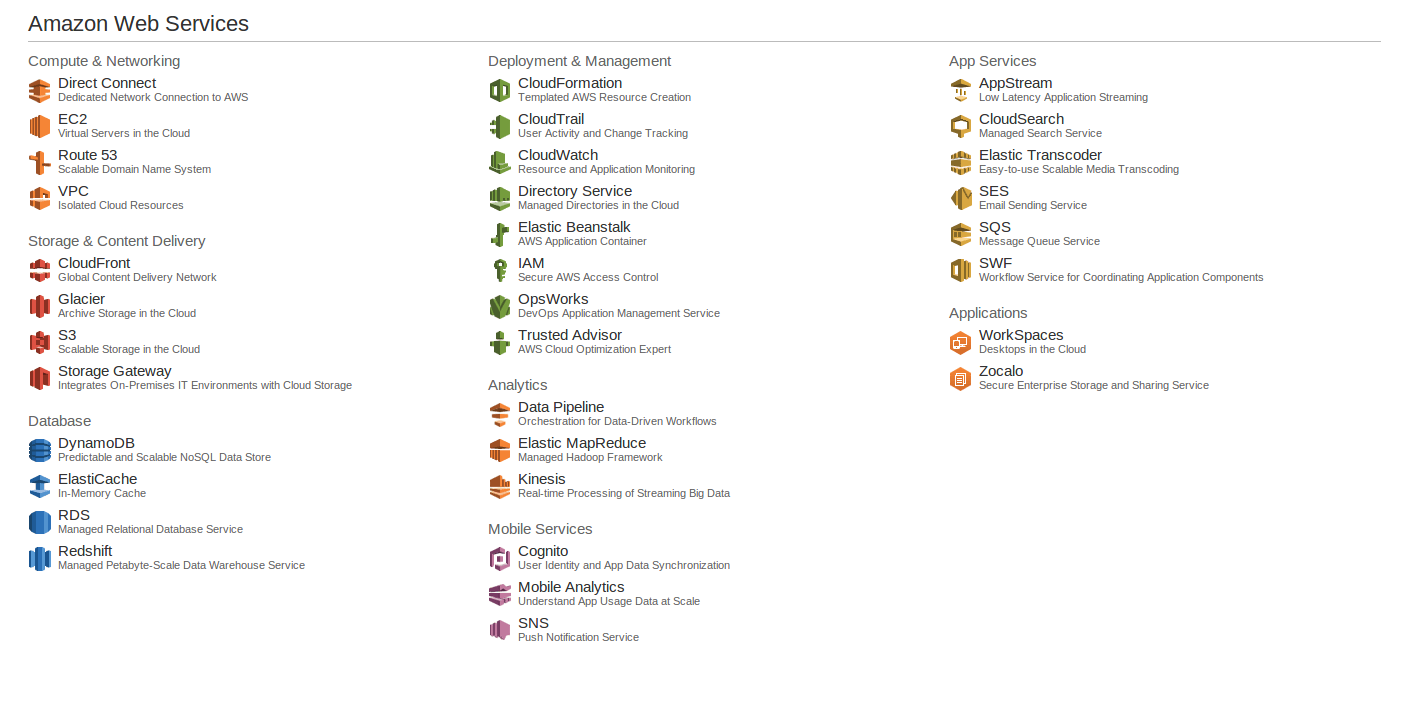
\includegraphics[width=1\textwidth]{img/aws_servicos}
%    \end{center}
%    \caption{Serviços da Amazon Web Services}
%    \label{fig:aws_servicos}
%\end{figure}
%
%\begin{figure}[htp]
%    \begin{center}
%    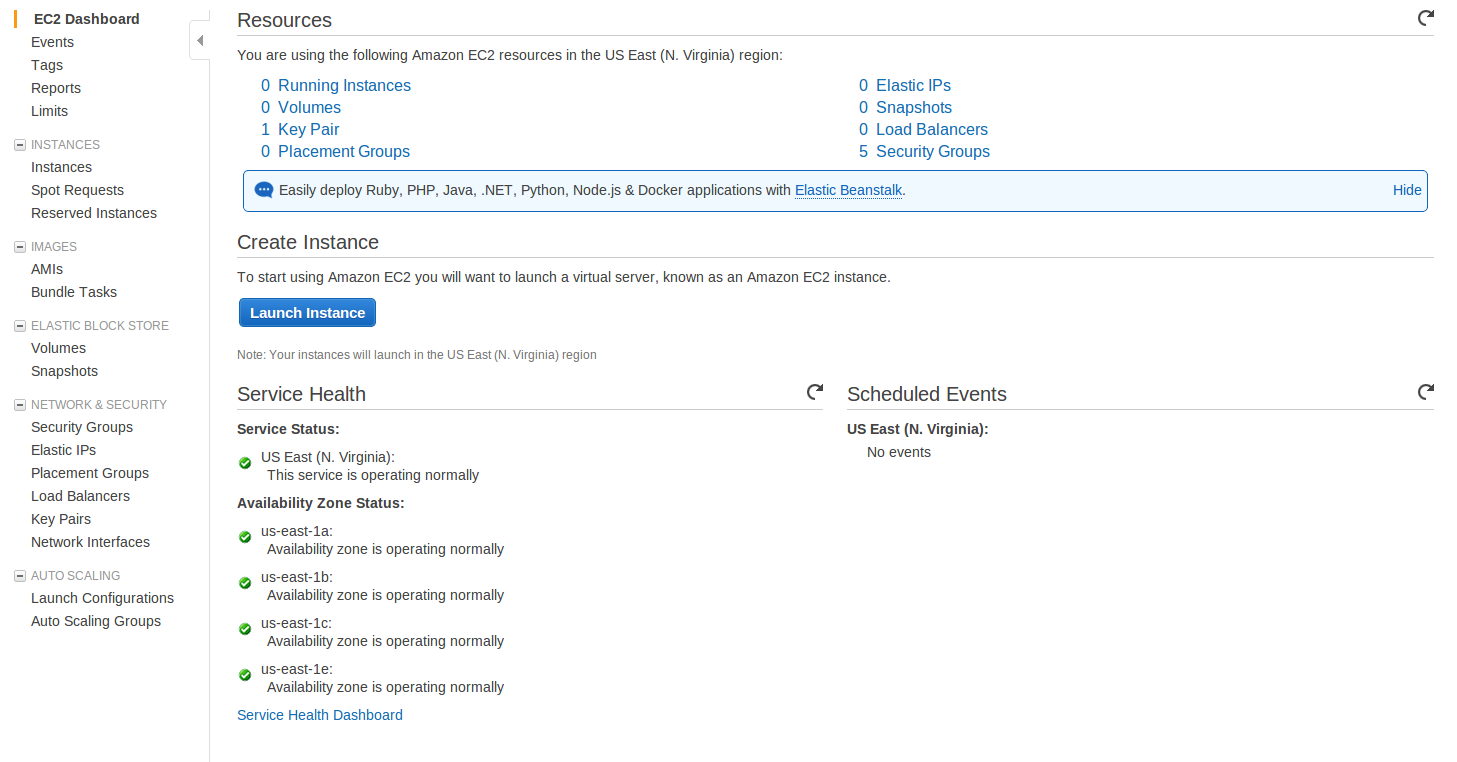
\includegraphics[width=1\textwidth]{img/aws_ec2}
%    \end{center}
%    \caption{Serviços de Elastic Compute Cloud (EC2)}
%    \label{fig:aws_ec2}
%\end{figure}
%
%\begin{figure}[htp]
%    \begin{center}
%    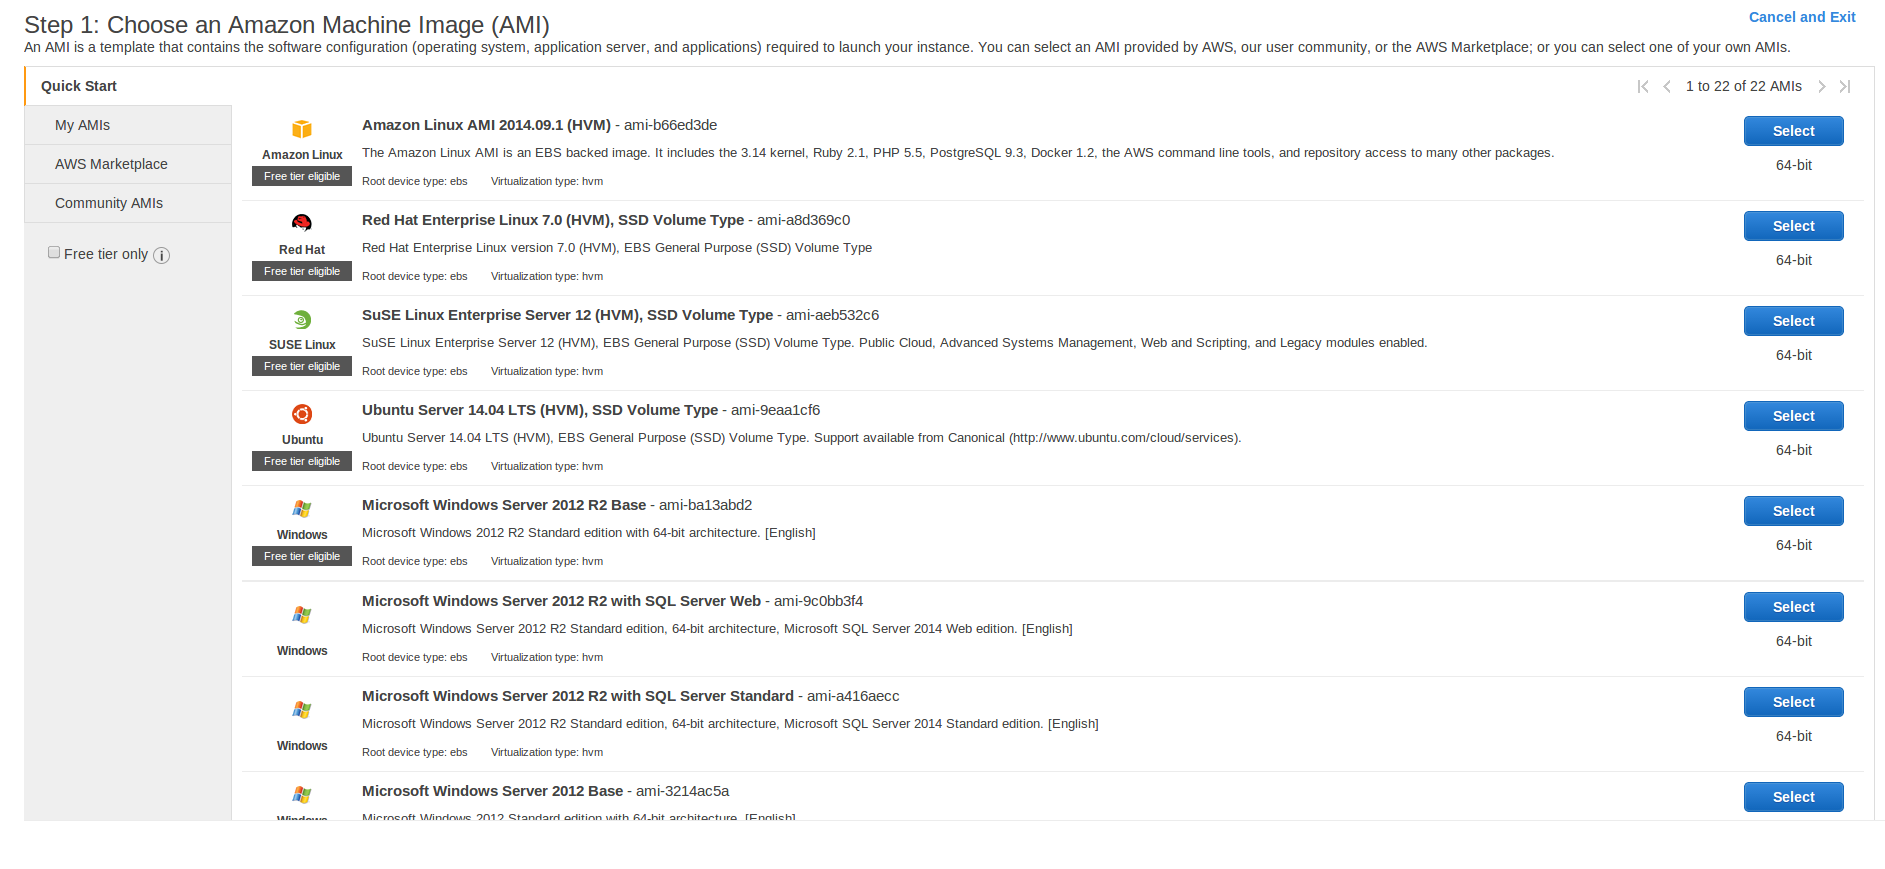
\includegraphics[width=1\textwidth]{img/aws_setup_ec2}
%    \end{center}
%    \caption{Escolha do tipo de configuração do software da máquina}
%    \label{fig:aws_setup_ec2}
%\end{figure}
%
%\begin{figure}[htp]
%    \begin{center}
%    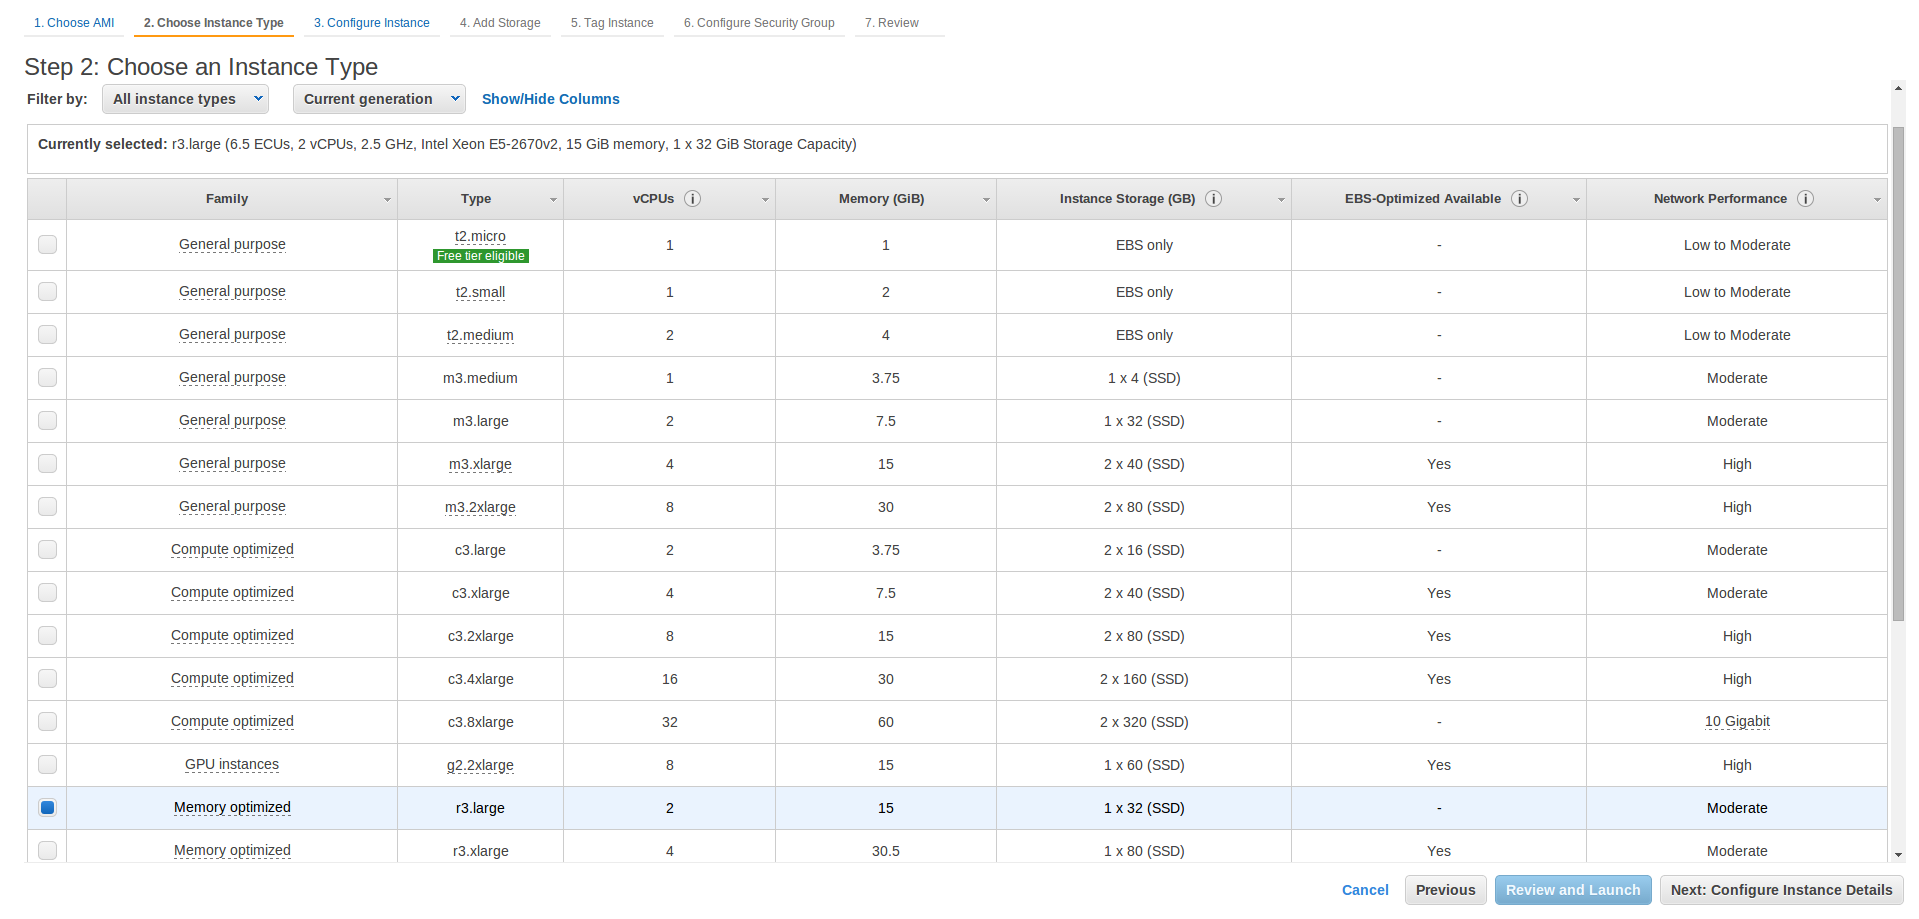
\includegraphics[width=1\textwidth]{img/aws_setup_ec2_maquina}
%    \end{center}
%    \caption{Escolha do tipo máquina}
%    \label{fig:aws_setup_ec2_maquina}
%\end{figure}
%
%\begin{figure}[htp]
%    \begin{center}
%    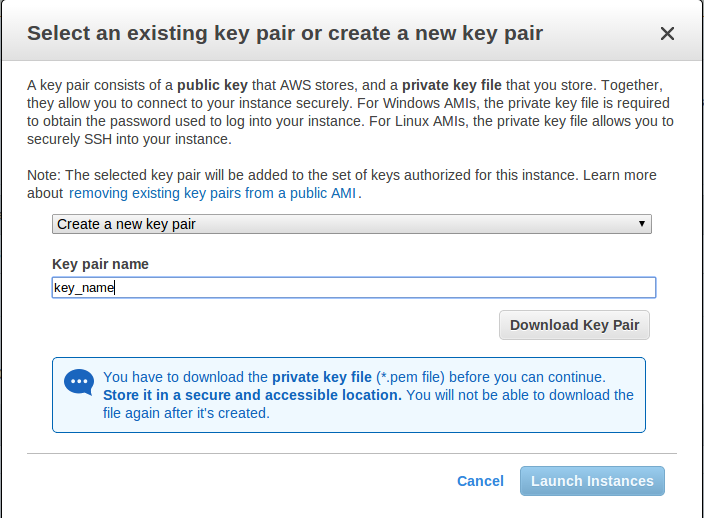
\includegraphics[width=1\textwidth]{img/aws_setup_keypair}
%    \end{center}
%    \caption{Criação da chave privada}
%    \label{fig:aws_setup_keypair}
%\end{figure}
%
%\begin{figure}[htp]
%    \begin{center}
%    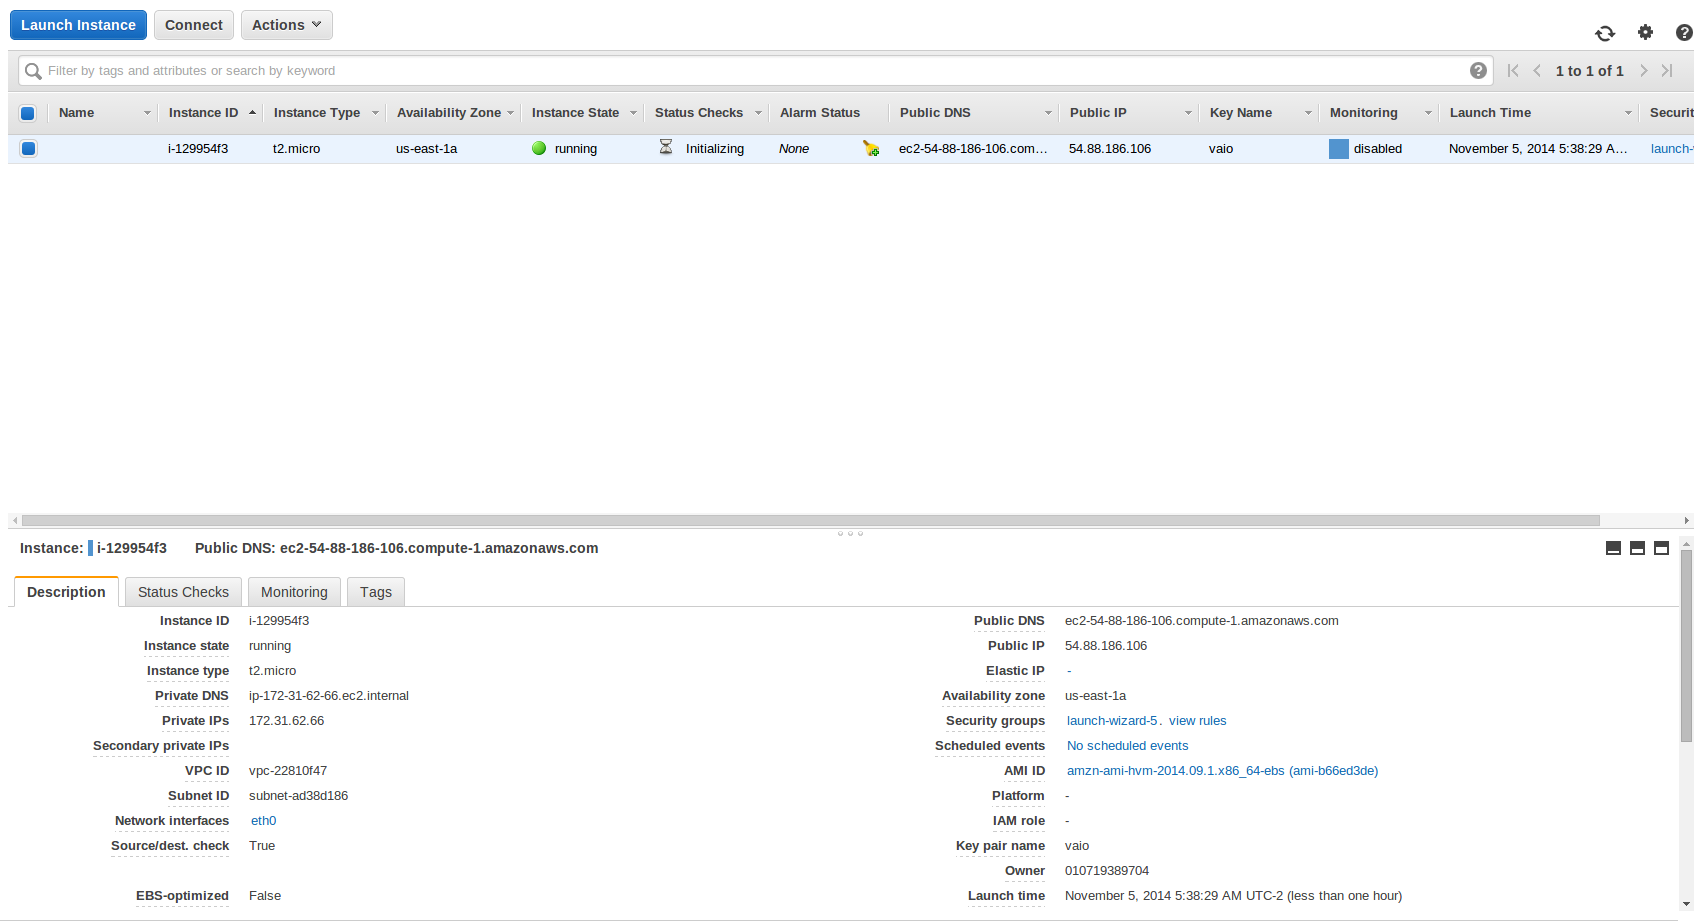
\includegraphics[width=1\textwidth]{img/aws_setup_dns}
%    \end{center}
%    \caption{Criação da máquina e do DNS público \textit{(Public DNS)}}
%    \label{fig:aws_setup_dns}
%\end{figure}



Uma vez criada a máquina, deve-se utilizar a chave privada para realizar um \textit{secure shell} e conectar-se remotamente ao EC2. A partir de um computador pessoal dotado de um interpretador de comandos \texttt{bash}, utilizamos a seguinte instrução:

%\begin{lstlisting}[caption=Secure shell para conexão com a máquina virtual EC2]
%ssh -i ~/Downloads/key_name.pem ec2-user@ec2-54-88-186-106.compute-1.amazonaws.com
%\end{lstlisting}

Em seguida, para a automatização do ambiente de testes e rápida configuração de novas máquinas, criamos um arquivo \texttt{script.sh} na linguagem de programação \texttt{bash}. Esse \textit{script} instala os pacotes \texttt{R} e \texttt{git} e cria a chave pública necessária para acessar o servidor onde o código da biblioteca está hospedado. Em virtude de sua popularidade, utilizamos o serviço de hospedagem de códigos abertos GitHub (\url{https://github.com/aviggiano/tcc}). 

\begin{lstlisting}[caption=\textit{Script} de configuração do ambiente de testes]
#!/usr/bin/env bash
sudo su						# login como administrador. necessario para instalar pacotes no sistema operacional
yes | yum install R		# instala o pacote R no linux
yes | yum install git	# instala o git para descarregar os metodos de recomendacao
ssh-keygen -t rsa			# gera a chave para conectar-se ao GitHub
cat ~/.ssh/id_rsa.pub	# imprime a chave publica, que deve ser adicionada nas configuracoes do GitHub
\end{lstlisting}

A saída do \textit{script} é uma chave pública.

Uma vez tendo habilitado a máquina virtual da AWS para manipulação do repositório da biblioteca, pode-se descarregar o código e executar o \textit{script} de testes de qualidade:

\begin{lstlisting}[caption=Script de execução dos testes de qualidade]
#!/usr/bin/env bash
git clone git@github.com:aviggiano/tcc	# clona o repositorio
cd tcc && Rscript recsys/results/run_tests.R 		# executa o script de testes
\end{lstlisting}
%%!TEX root = index.tex
\section[Resultados]{Resultados}

\begin{frame}{Resultados}
\begin{table}[hp]
\begin{center}
    \caption{Parâmetros de influência no desempenho dos algoritmos de recomendação}\vspace{-.5cm}
    \label{tab:variaveis}
    \begin{tabular}{  | p{1.5cm} | p{5.5cm} | p{3.0cm} | } 
    \hline
    \textbf{Variável} & \textbf{Descrição} & \textbf{Valor padrão}  \\ \hline
    $N$ & Lista de recomendação & $20$ \\ \hline   
    $T$ & Base de treinamento & $75\%$ \\ \hline
    $H$ & Avaliações ``escondidas'' & $75\%$ \\ \hline
    $d^f$ & Medida de distância & Distância $L_1$~$\left|\left|\cdot\right|\right|^f$ \\ \hline
    $\mathcal{F}$ & Conjunto de atributos dos itens & Todos atributos \\ \hline
    $M$ & Avaliações positivas & $2$ \\ \hline
    $k$ & Vizinhos mais próximos & $10$ \\ \hline
    $W$ & Quantidade de pesos & Todo $w_f>0$ \\ \hline
    \end{tabular}
\end{center}
\end{table}
\end{frame}

\begin{frame}{Resultados}{Tamanho da lista de recomendação $N$}

\begin{columns}[b]
\column{.5\textwidth} %
\begin{figure}[ht]
    \begin{center}
    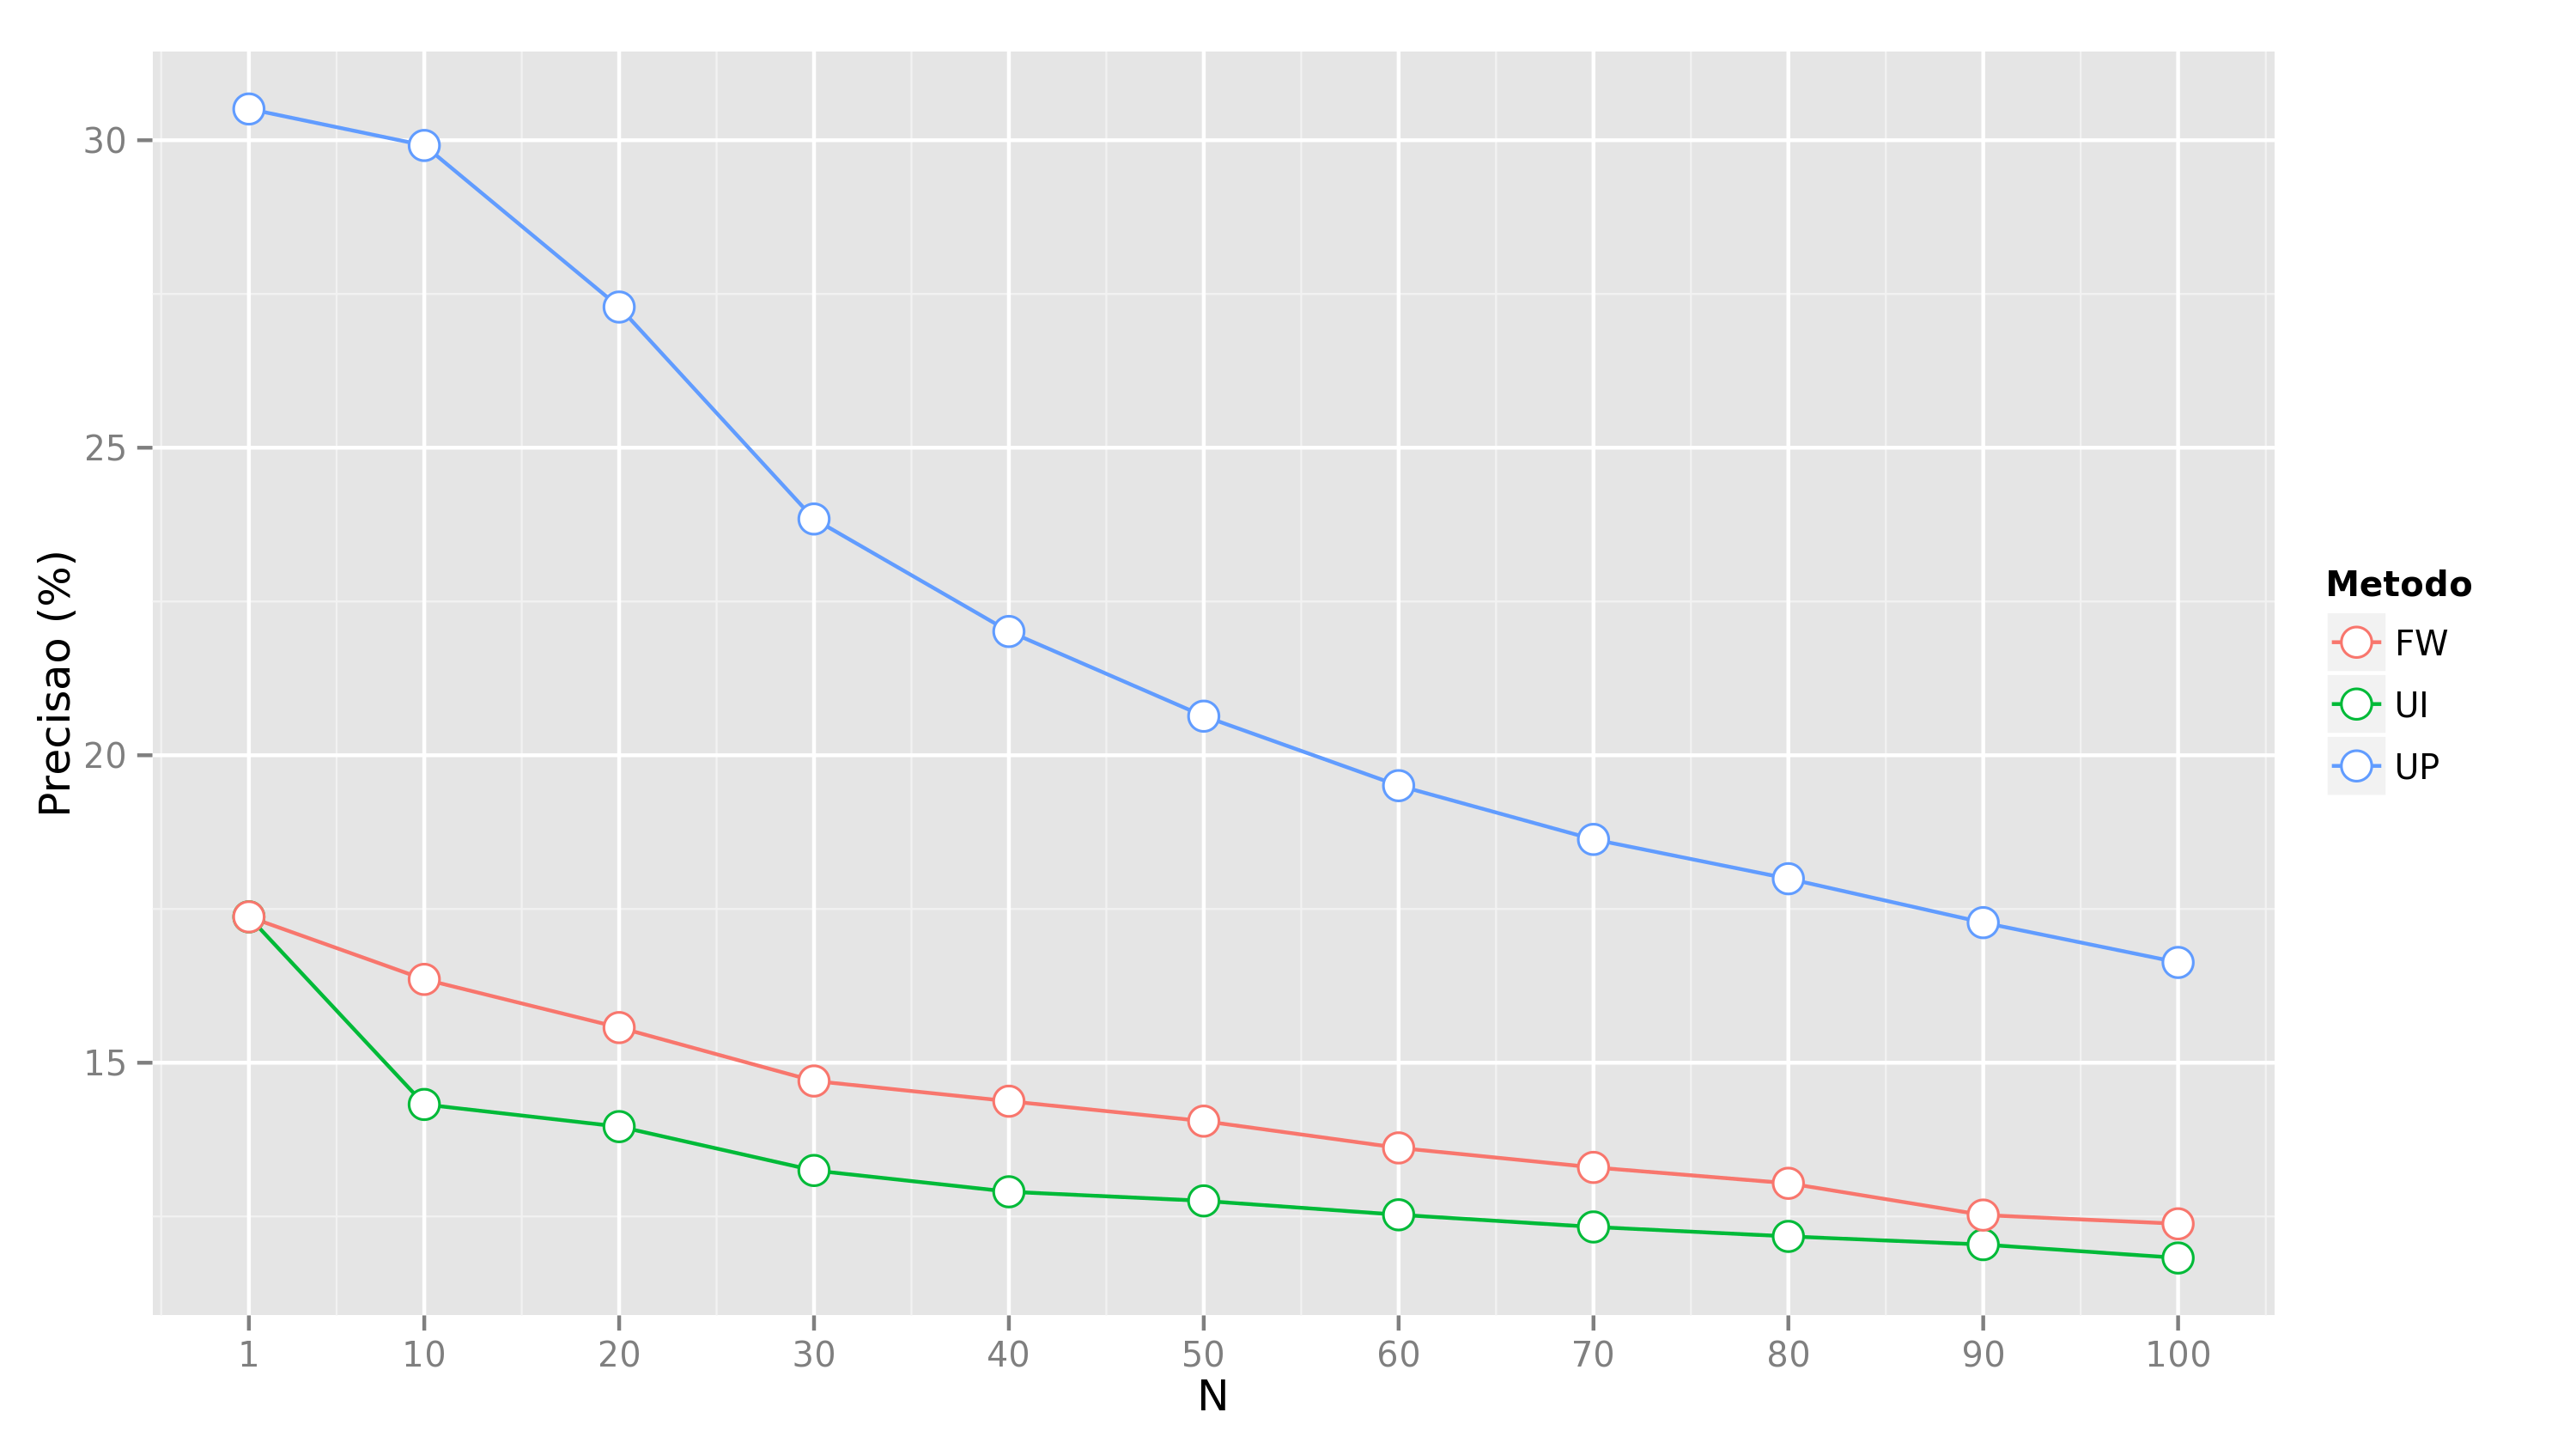
\includegraphics[width=1.1\textwidth]{../img/precision_N}
    \end{center}
    \caption{Precisão $\times$ $N$}
    \label{fig:precision_N}
\end{figure}

\column{.5\textwidth} % 

\begin{figure}[ht]
    \begin{center}
    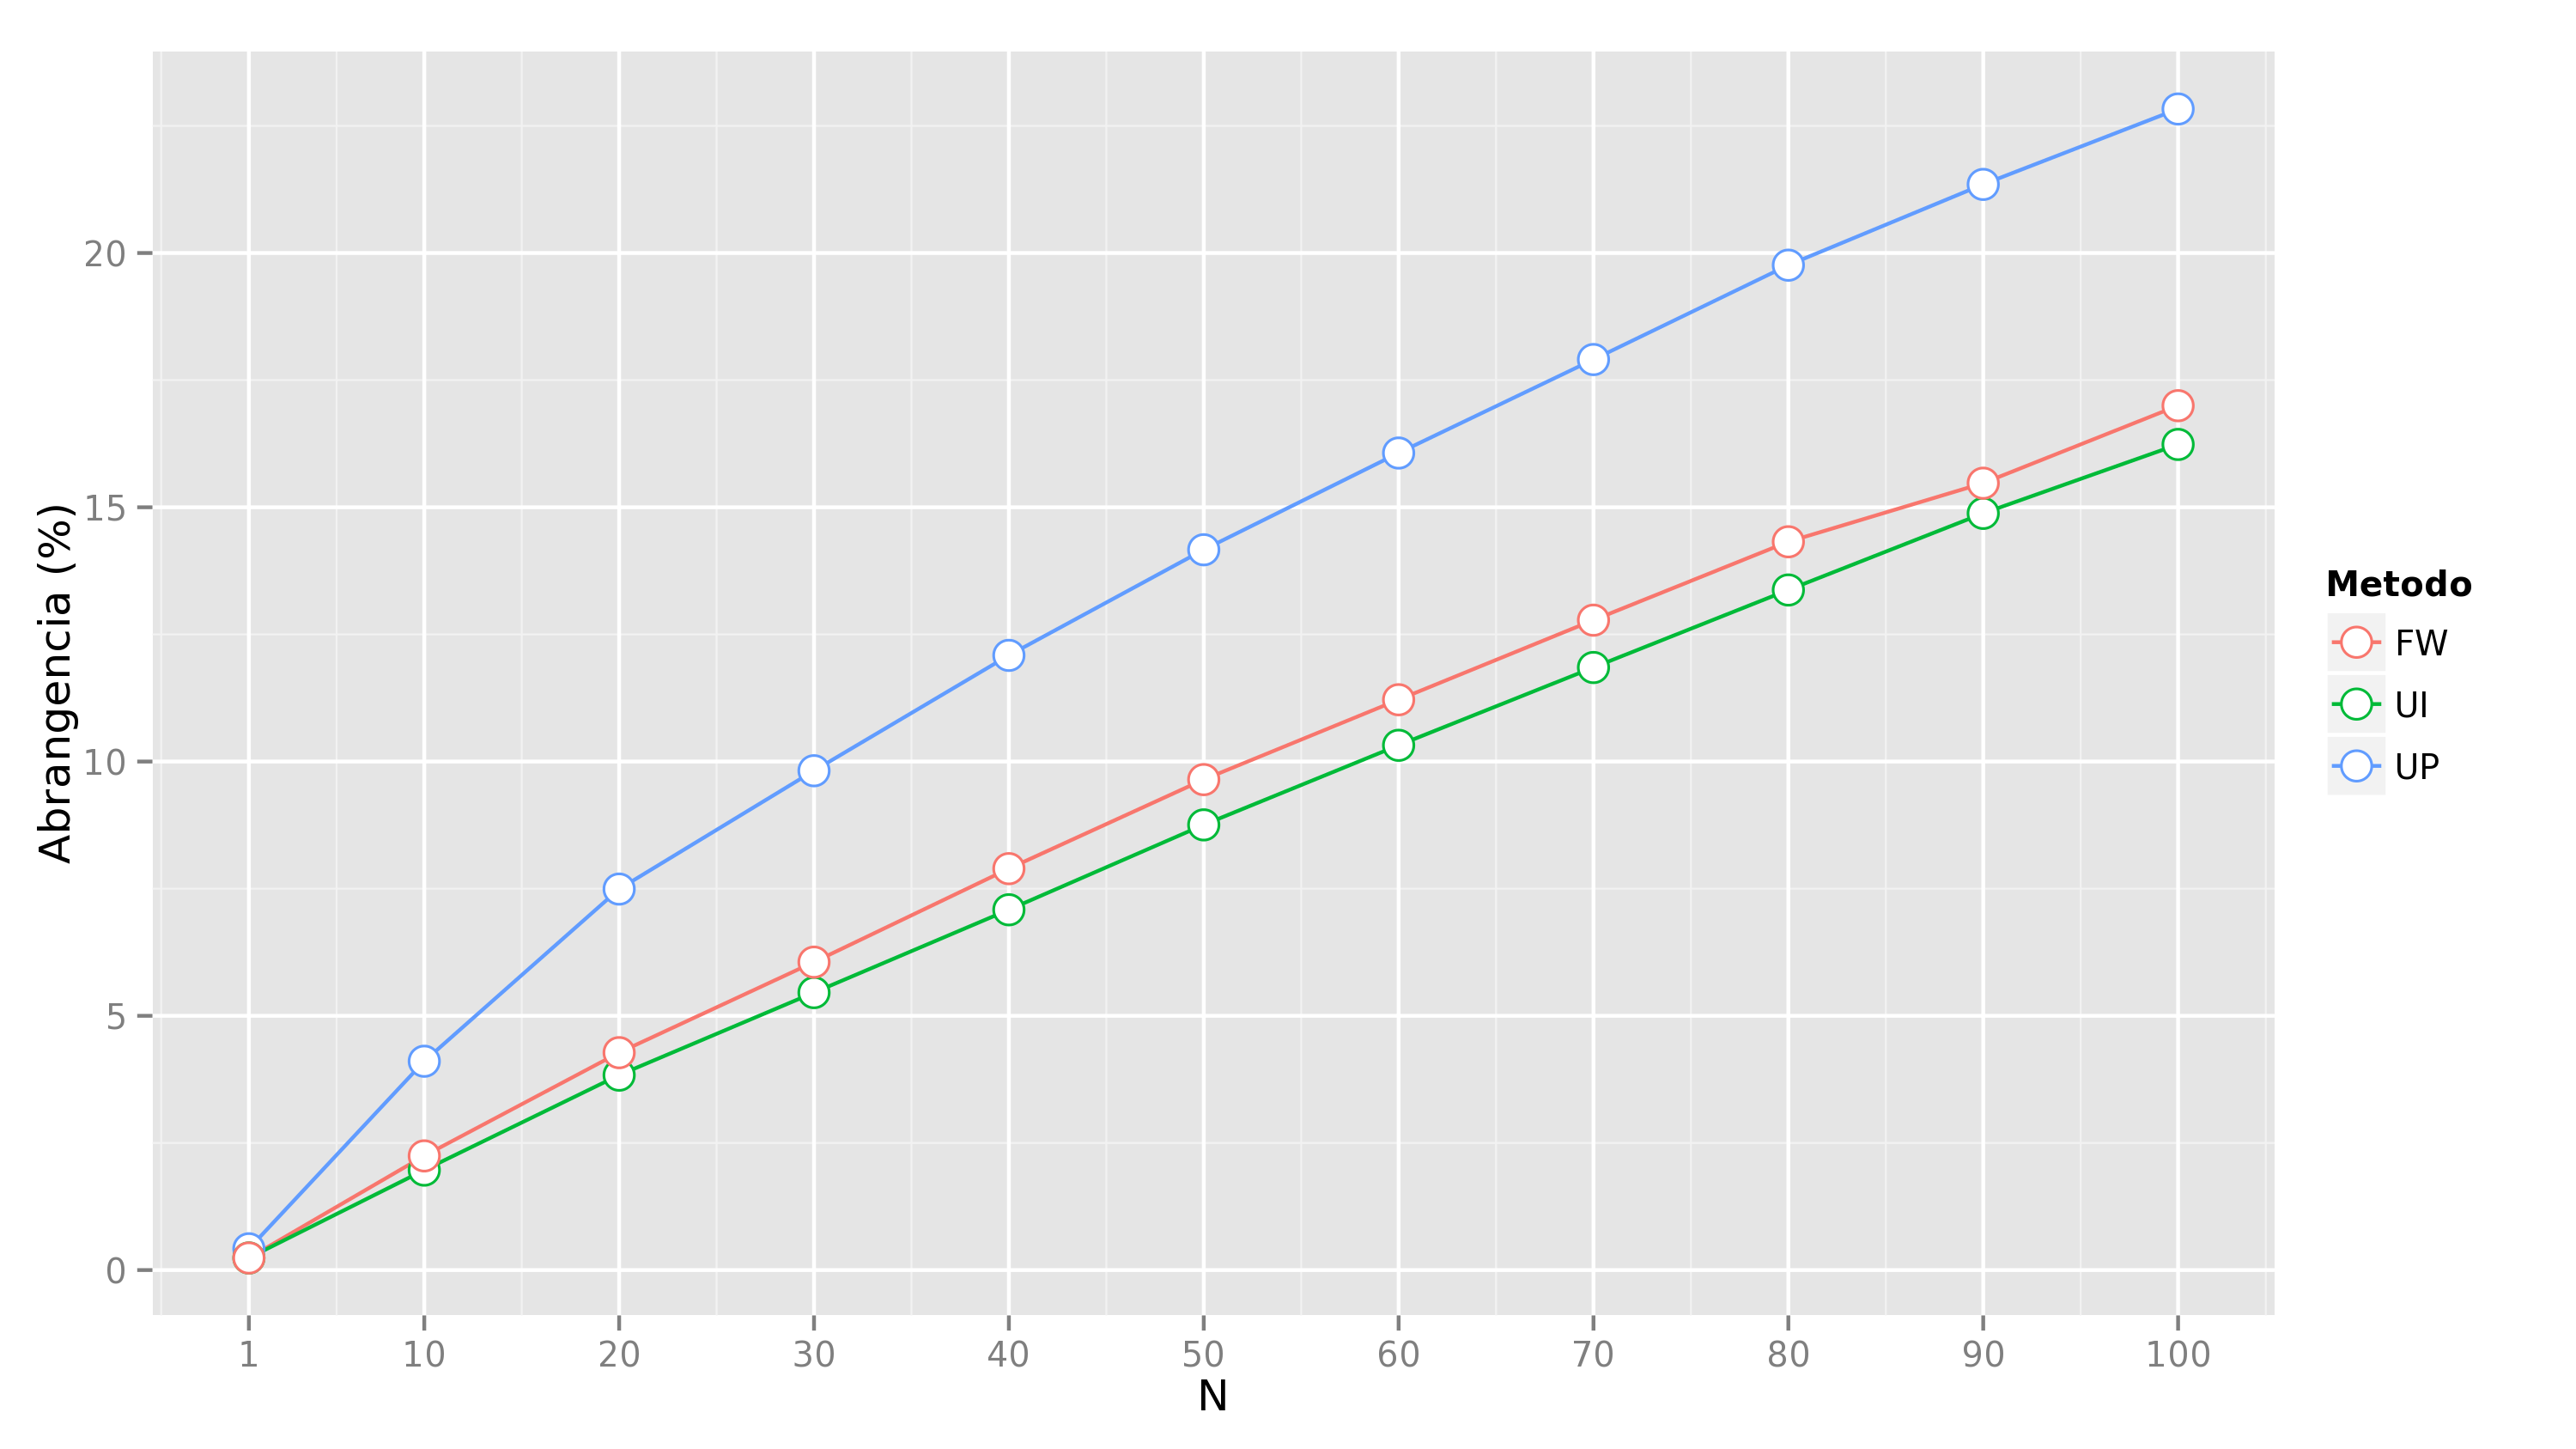
\includegraphics[width=1.1\textwidth]{../img/recall_N}
    \end{center}
    \caption{Abrangência $\times$ $N$}
    \label{fig:recall_N}
\end{figure}
\end{columns}
\end{frame}

\begin{frame}{Resultados}{Tamanho da lista de recomendação $N$}
\begin{columns}[b]
\column{.5\textwidth} %
\begin{figure}[ht]
    \begin{center}
    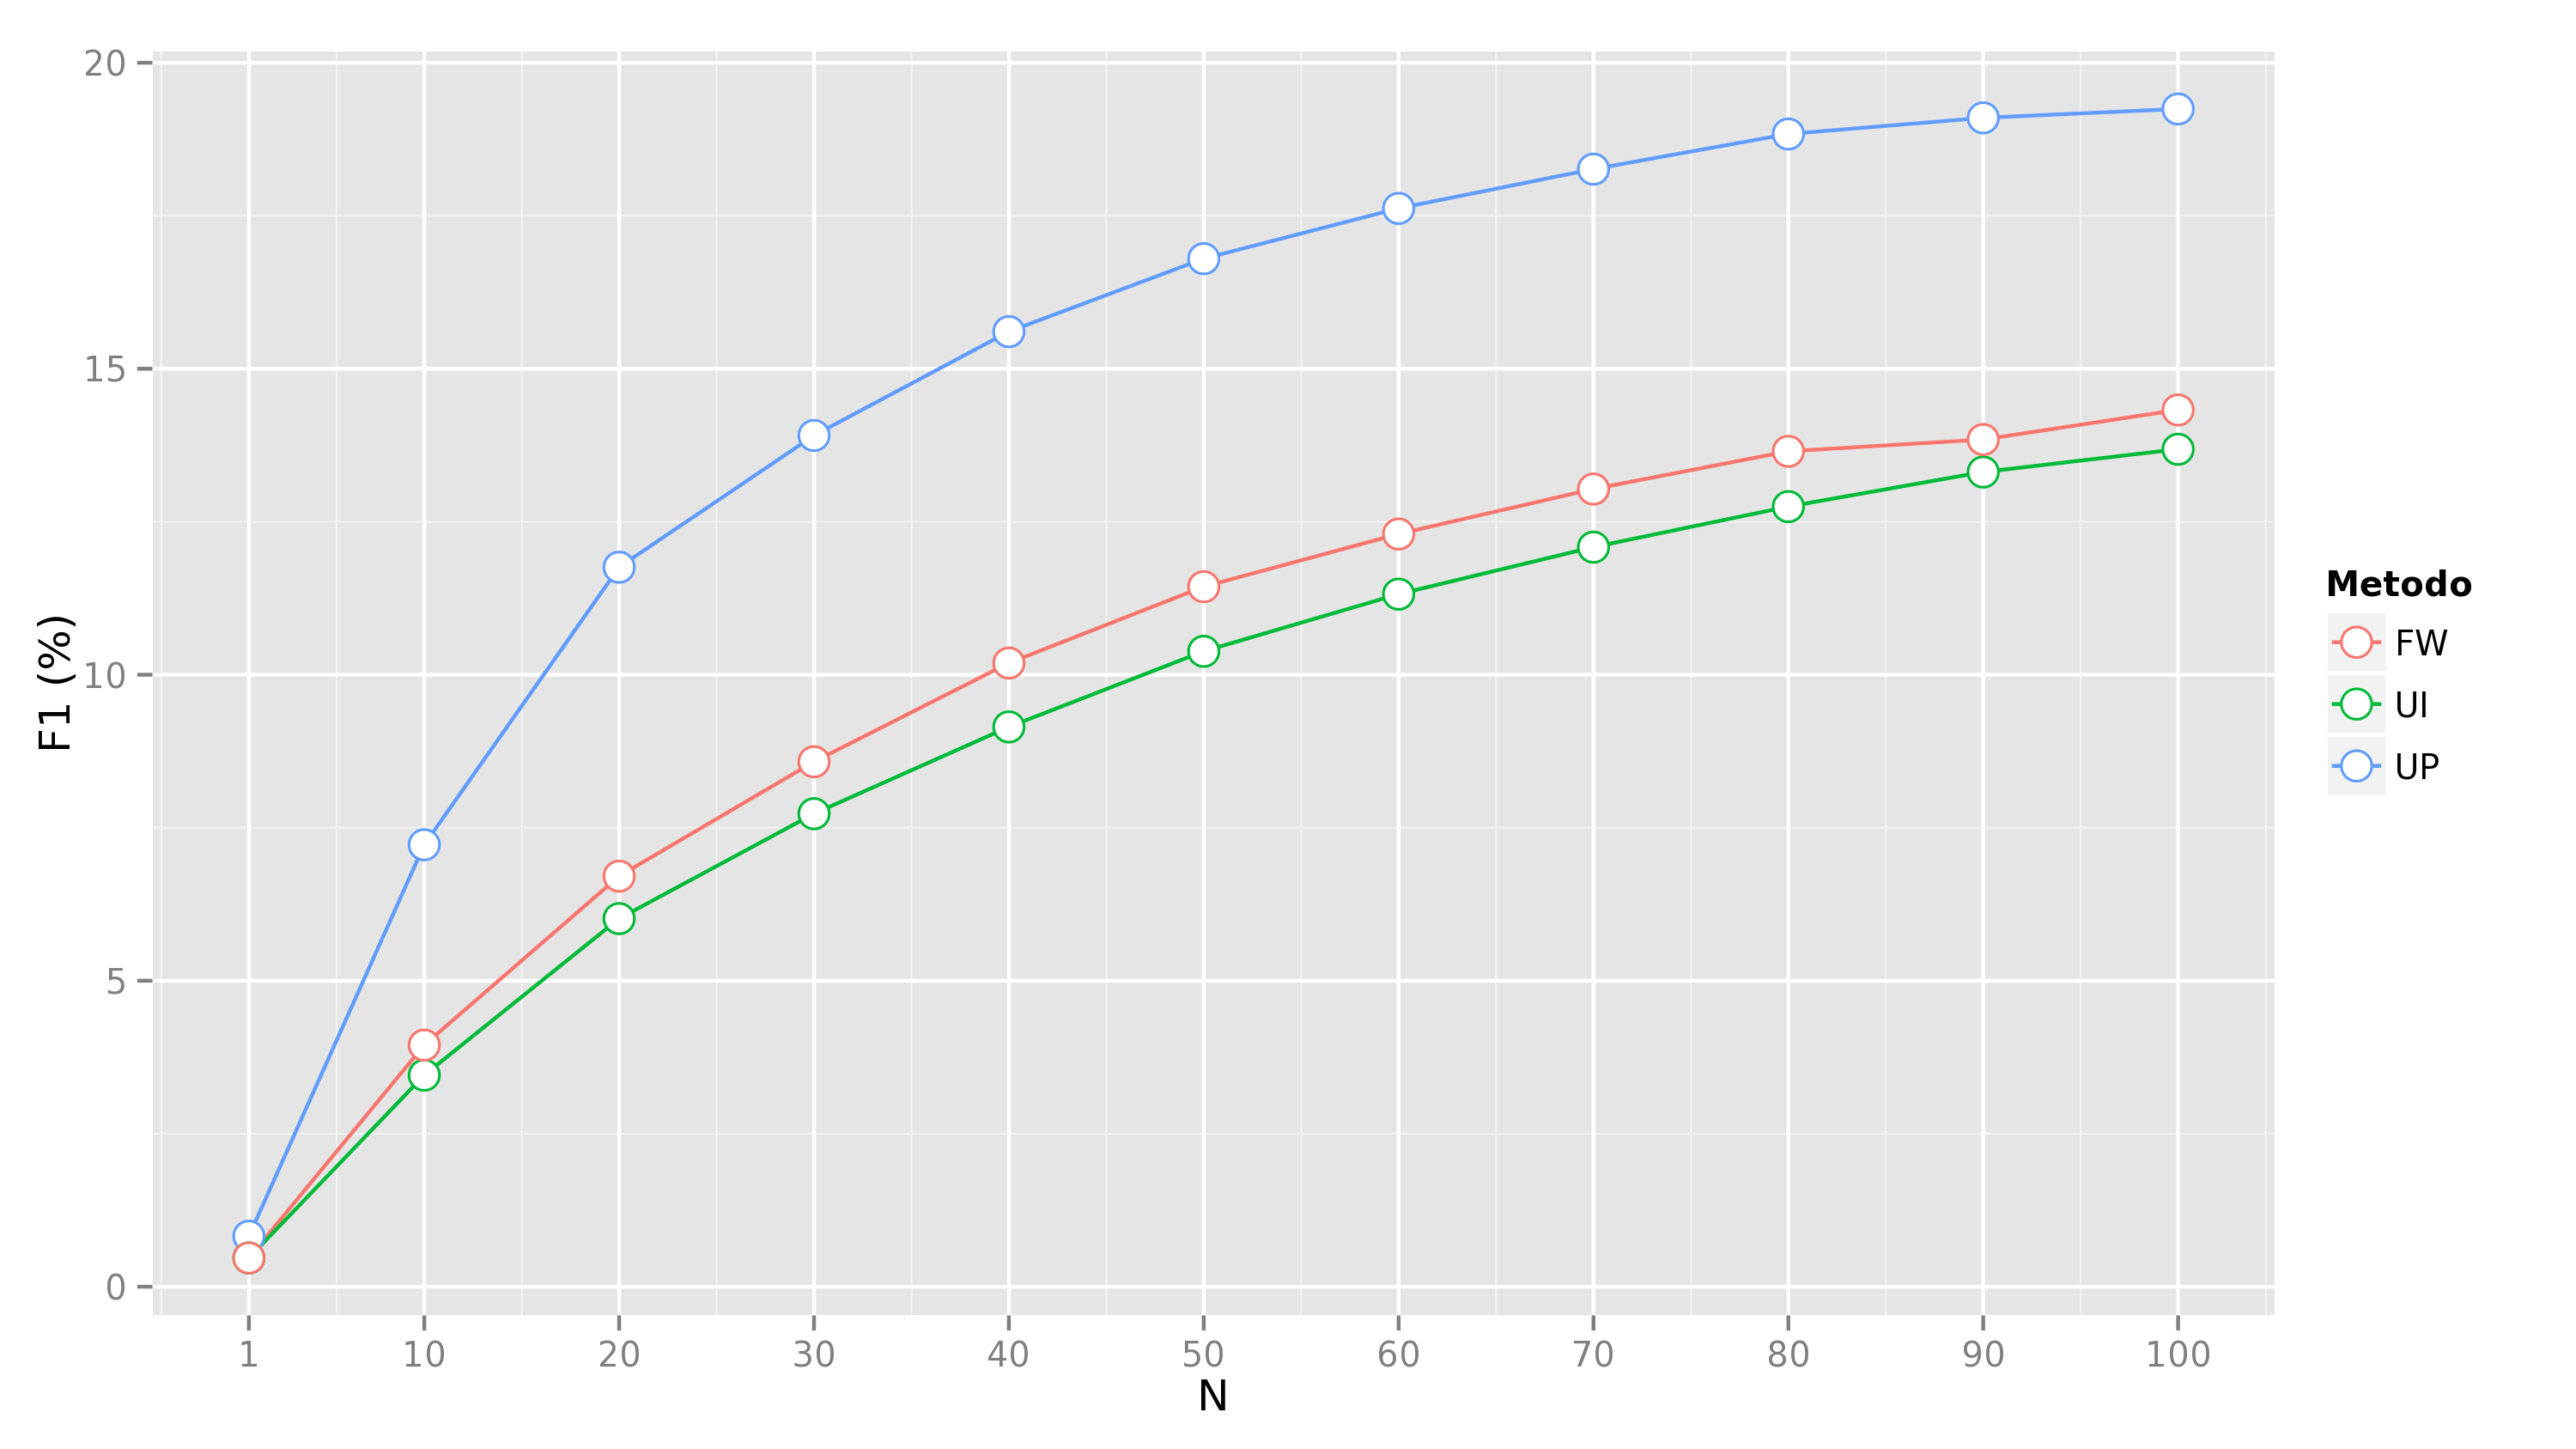
\includegraphics[width=1.1\textwidth]{../img/F1_N}
    \end{center}
    \caption{$F_1$ $\times$ $N$}
    \label{fig:F1_N}
\end{figure}

\column{.5\textwidth} % 

\begin{figure}[ht]
    \begin{center}
    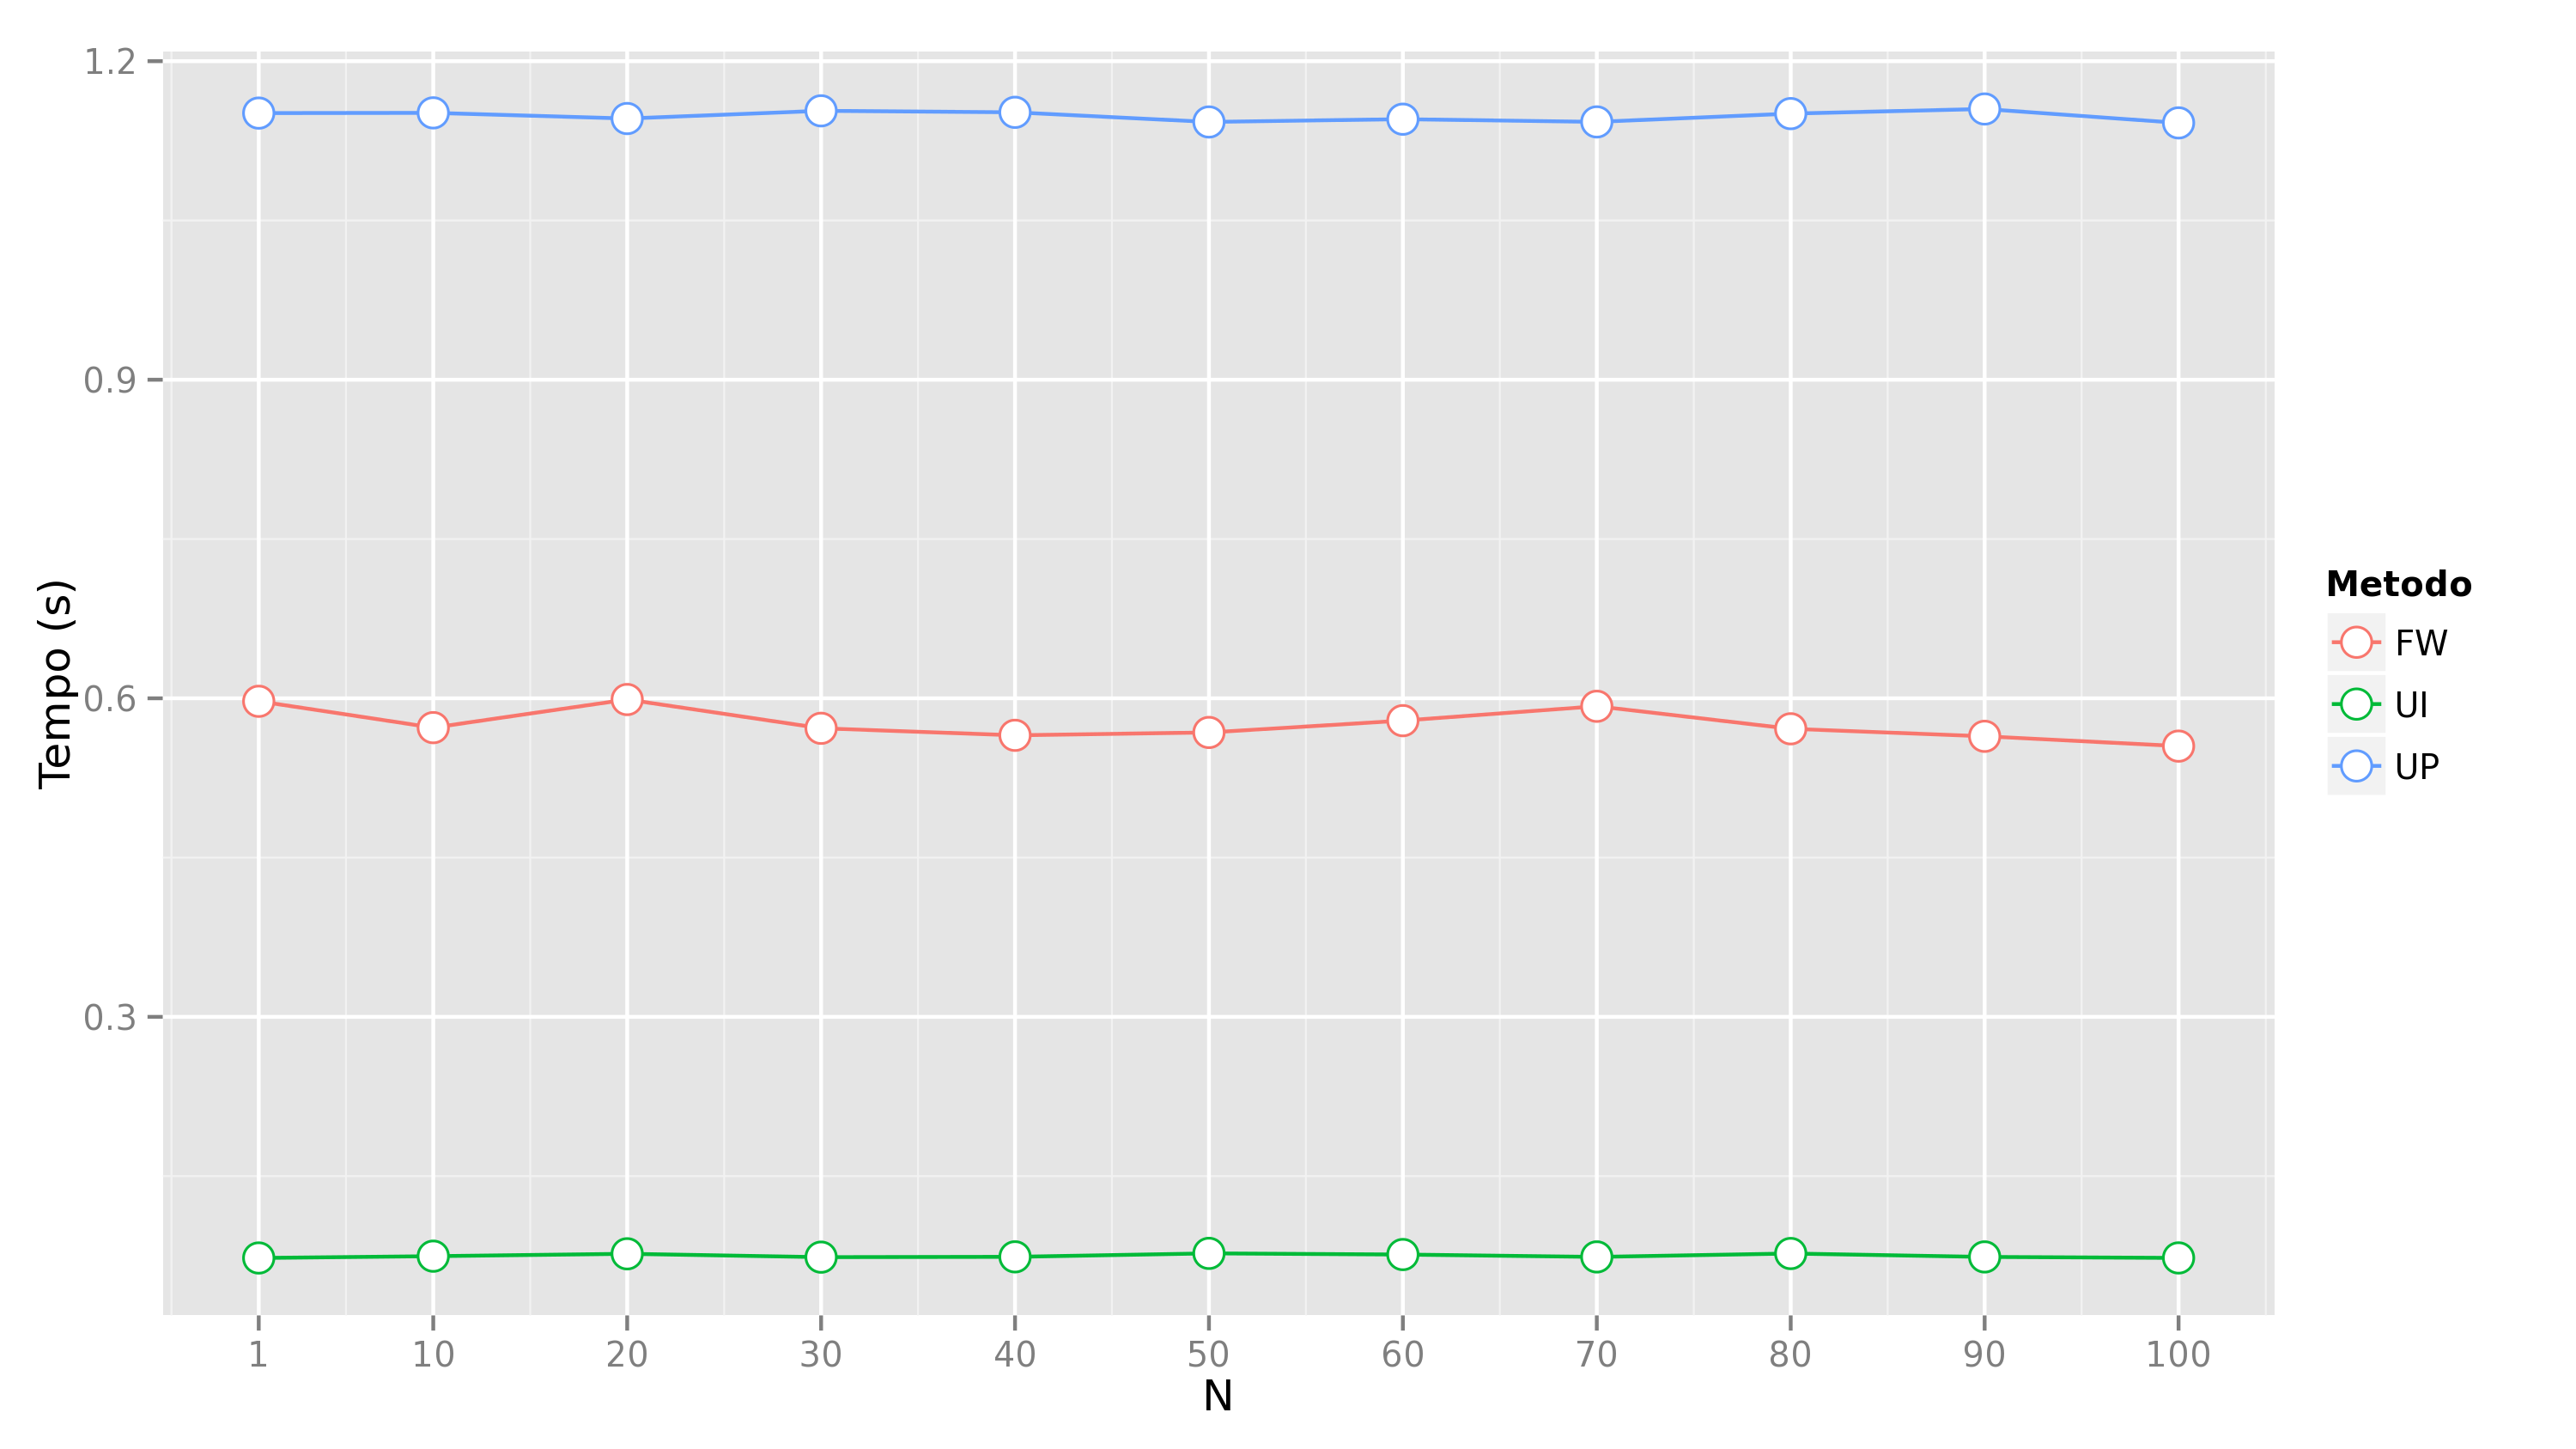
\includegraphics[width=1.1\textwidth]{../img/time_N}
    \end{center}
    \caption{Tempo $\times$ $N$}
    \label{fig:time_N}
\end{figure}
\end{columns}
\end{frame}

\begin{frame}{Resultados}{Percentual da base de aprendizado $T$}
\begin{figure}[ht]
    \begin{center}
    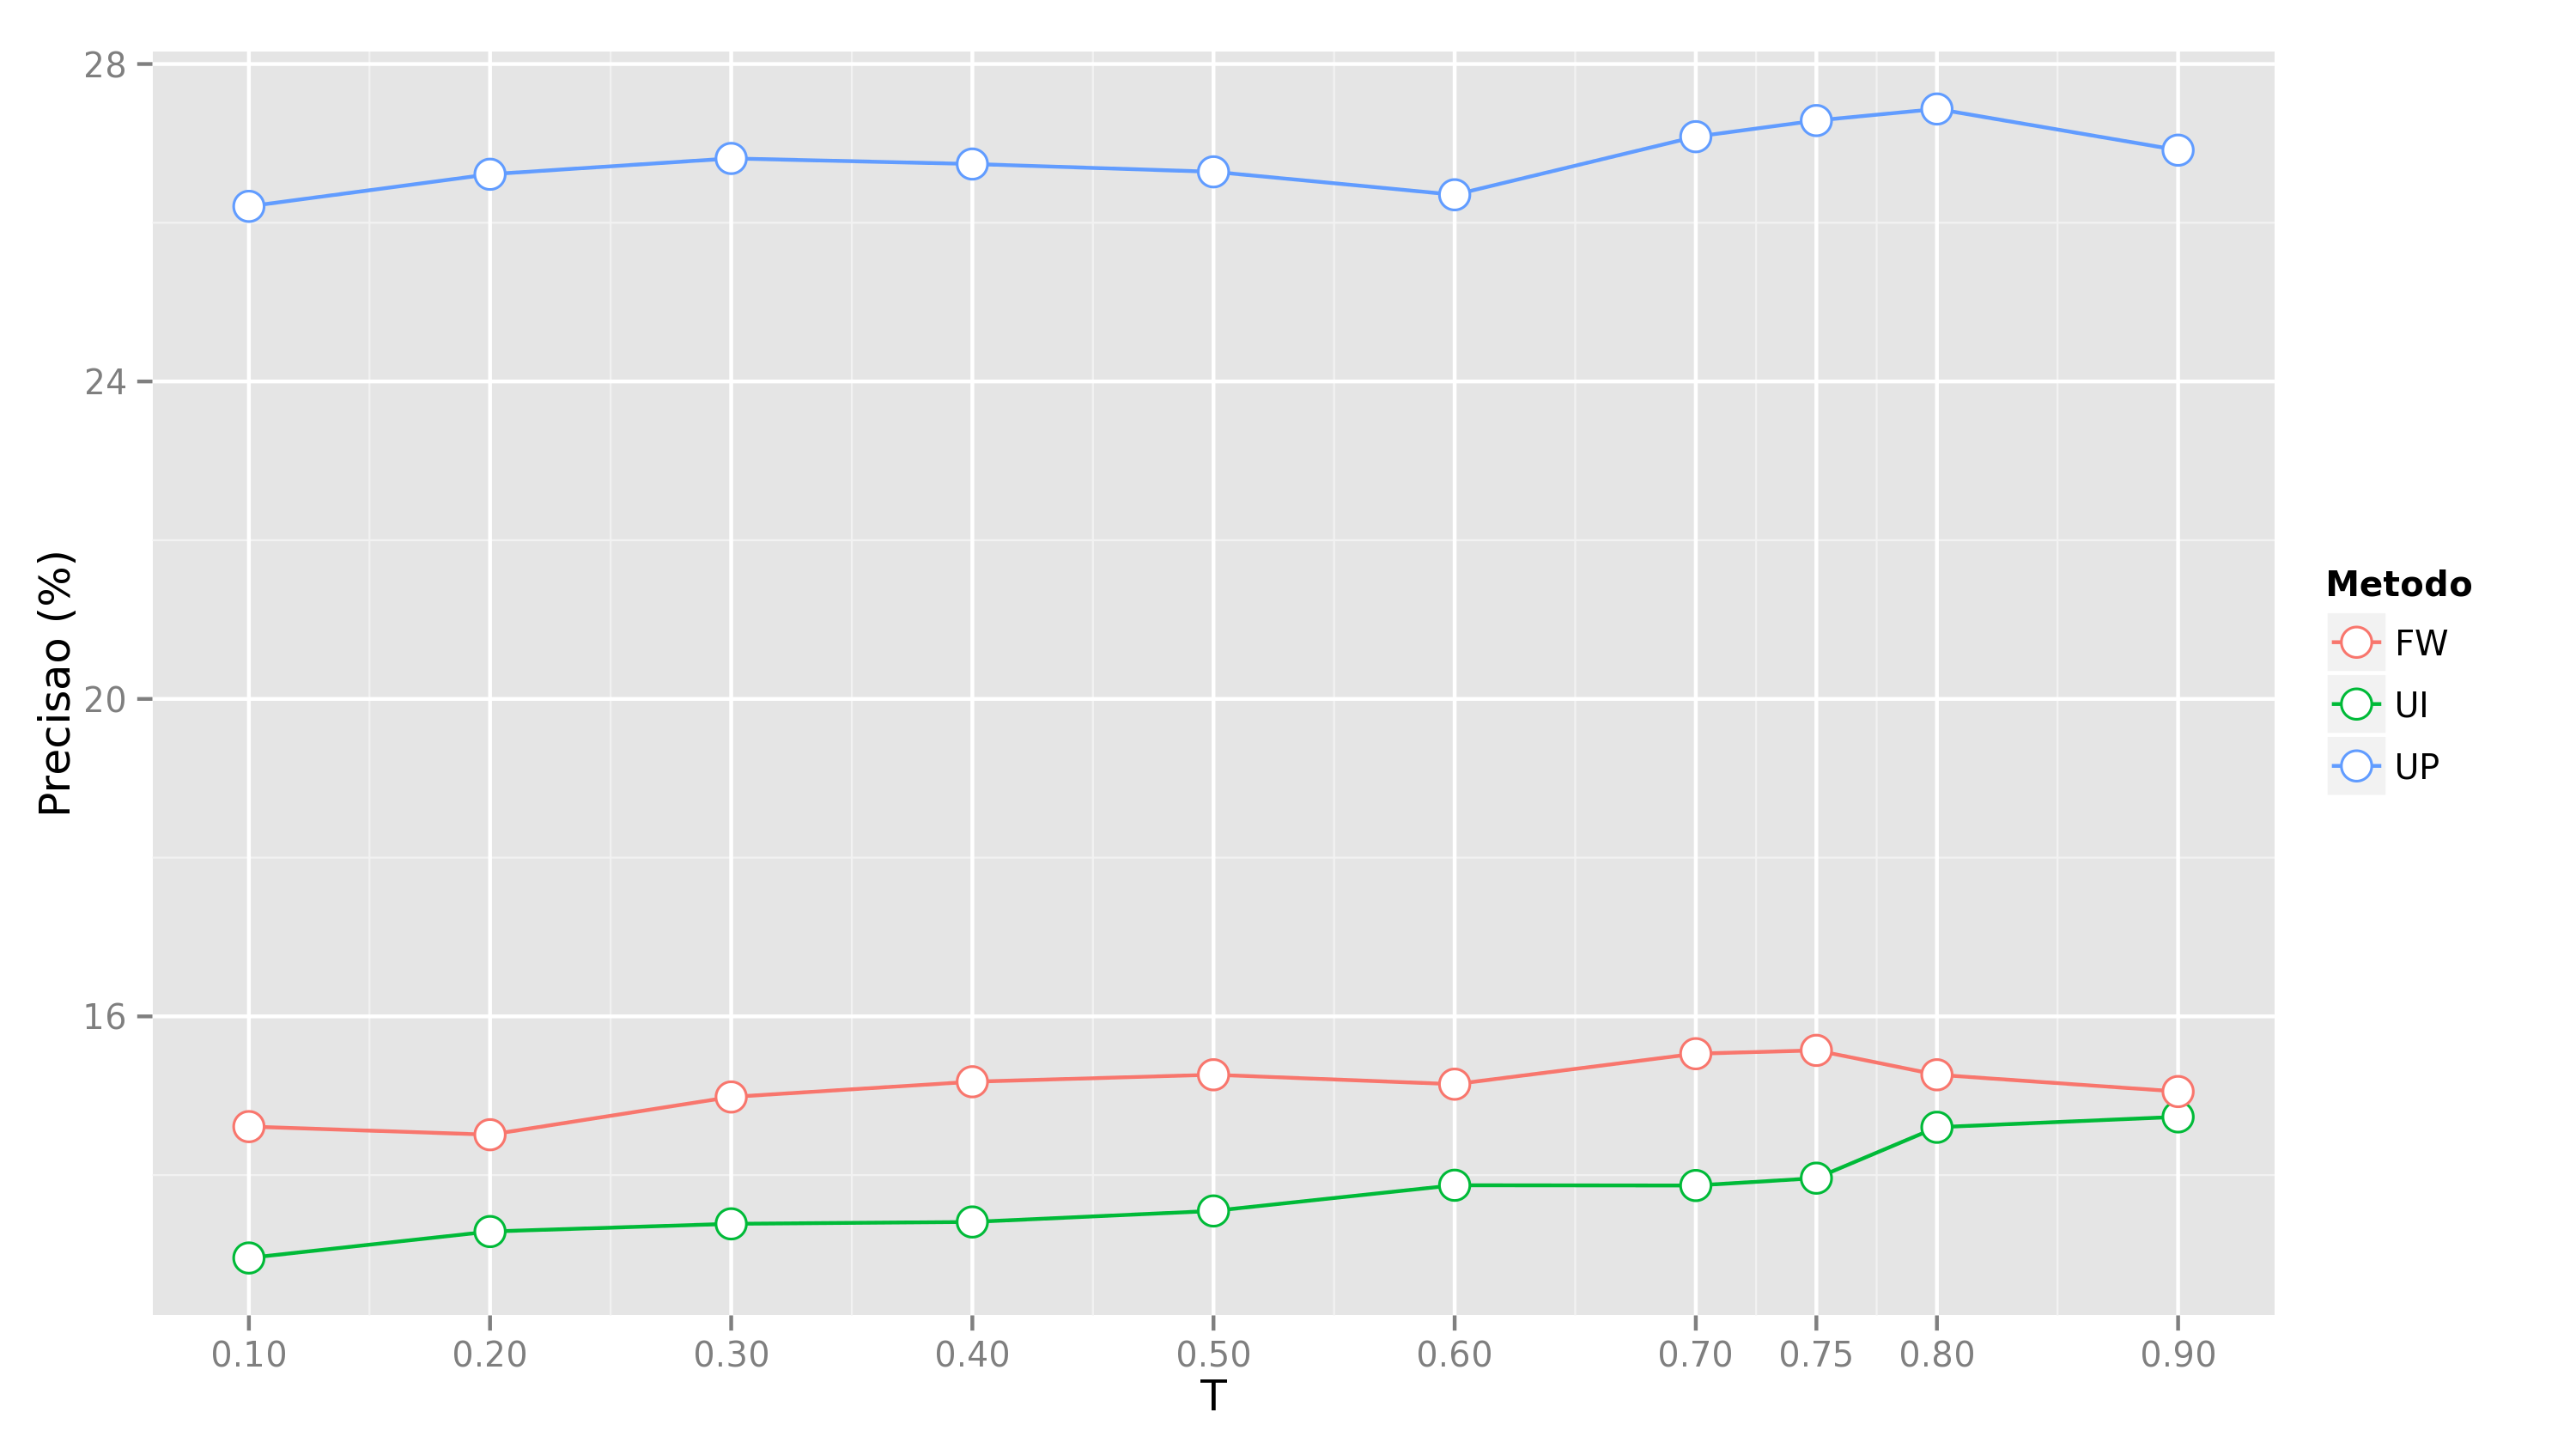
\includegraphics[width=.8\textwidth]{../img/precision_T}
    \end{center}
    \caption{Precisão $\times$ $T$}
    \label{fig:precision_T}
\end{figure}
\begin{center}
    Abrangência, $F_1$ e Tempo praticamente constantes
\end{center}
\end{frame}

\begin{frame}{Resultados}{Percentual de avaliações ``escondidas'' dos usuários-teste $H$}
\begin{figure}[ht]
    \begin{center}
    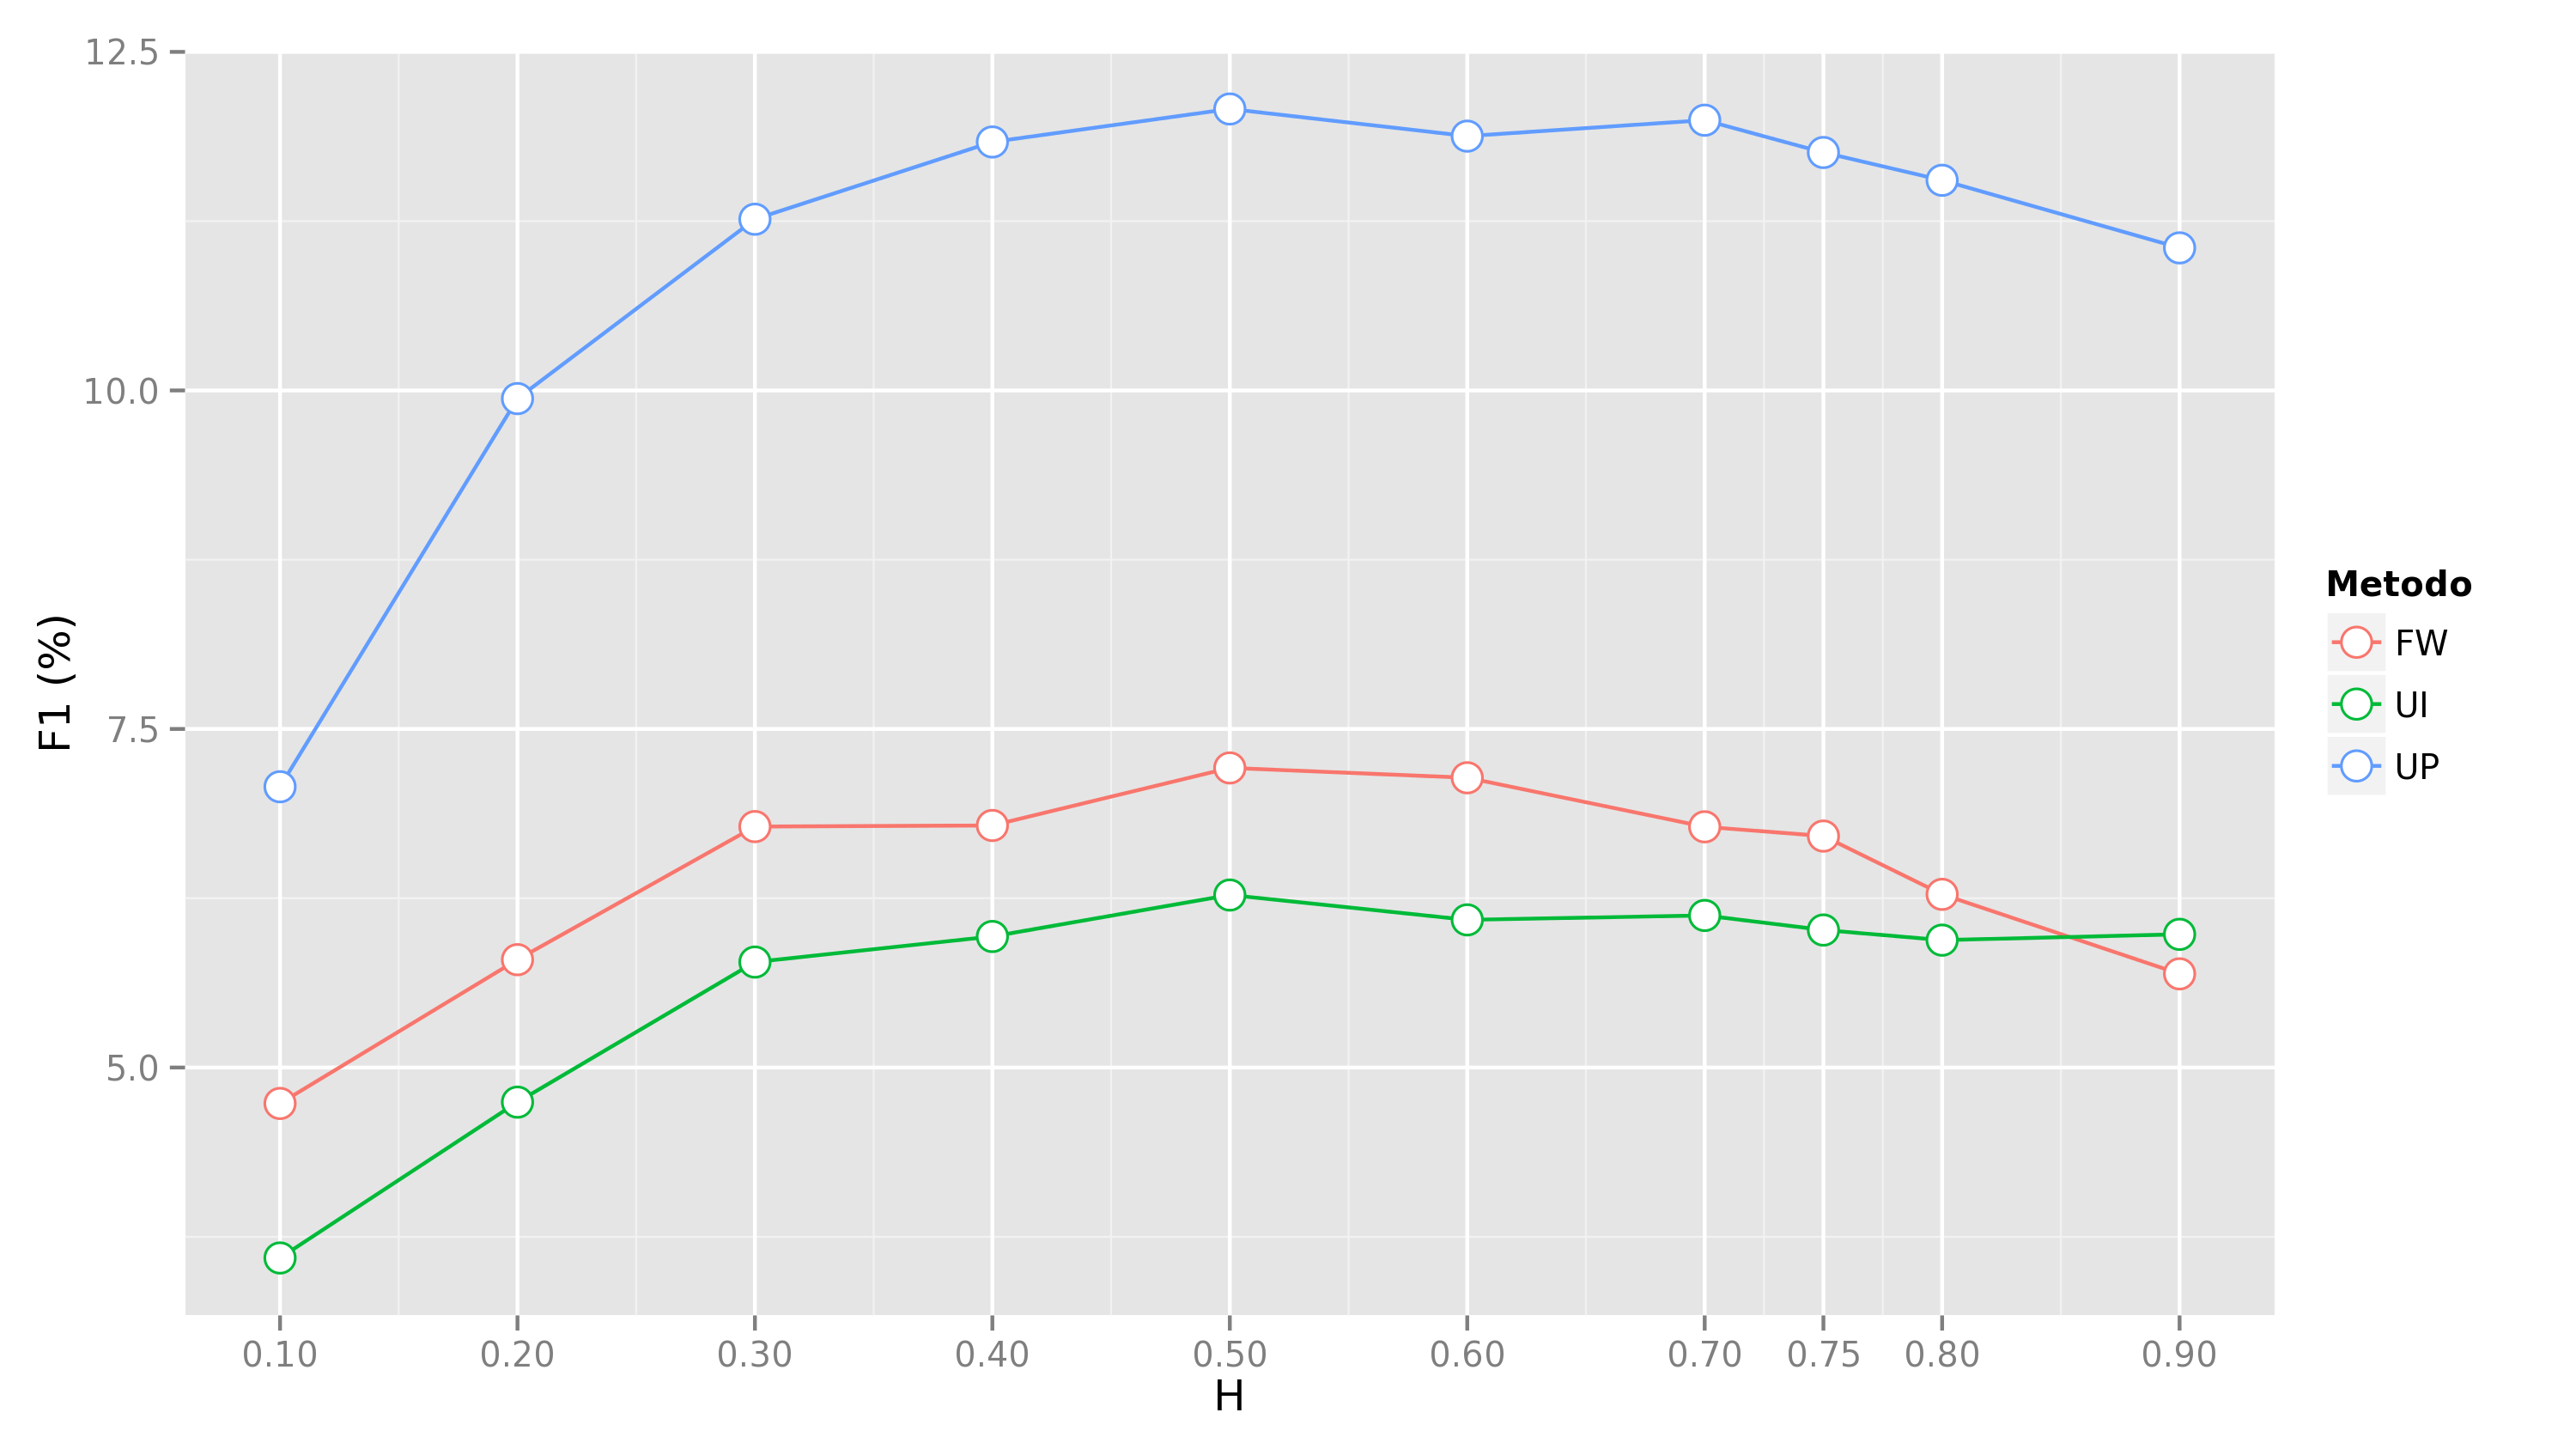
\includegraphics[width=.8\textwidth]{../img/F1_H}
    \end{center}
    \caption{$F_1$ $\times$ $H$}
    \label{fig:F1_H}
\end{figure}
\begin{center}
    Precisão cresce e Abrangência decresce
\end{center}
\end{frame}


\begin{frame}{Resultados}{Medida de distância entre atributos $d^f$}
\begin{figure}[ht]
    \begin{center}
    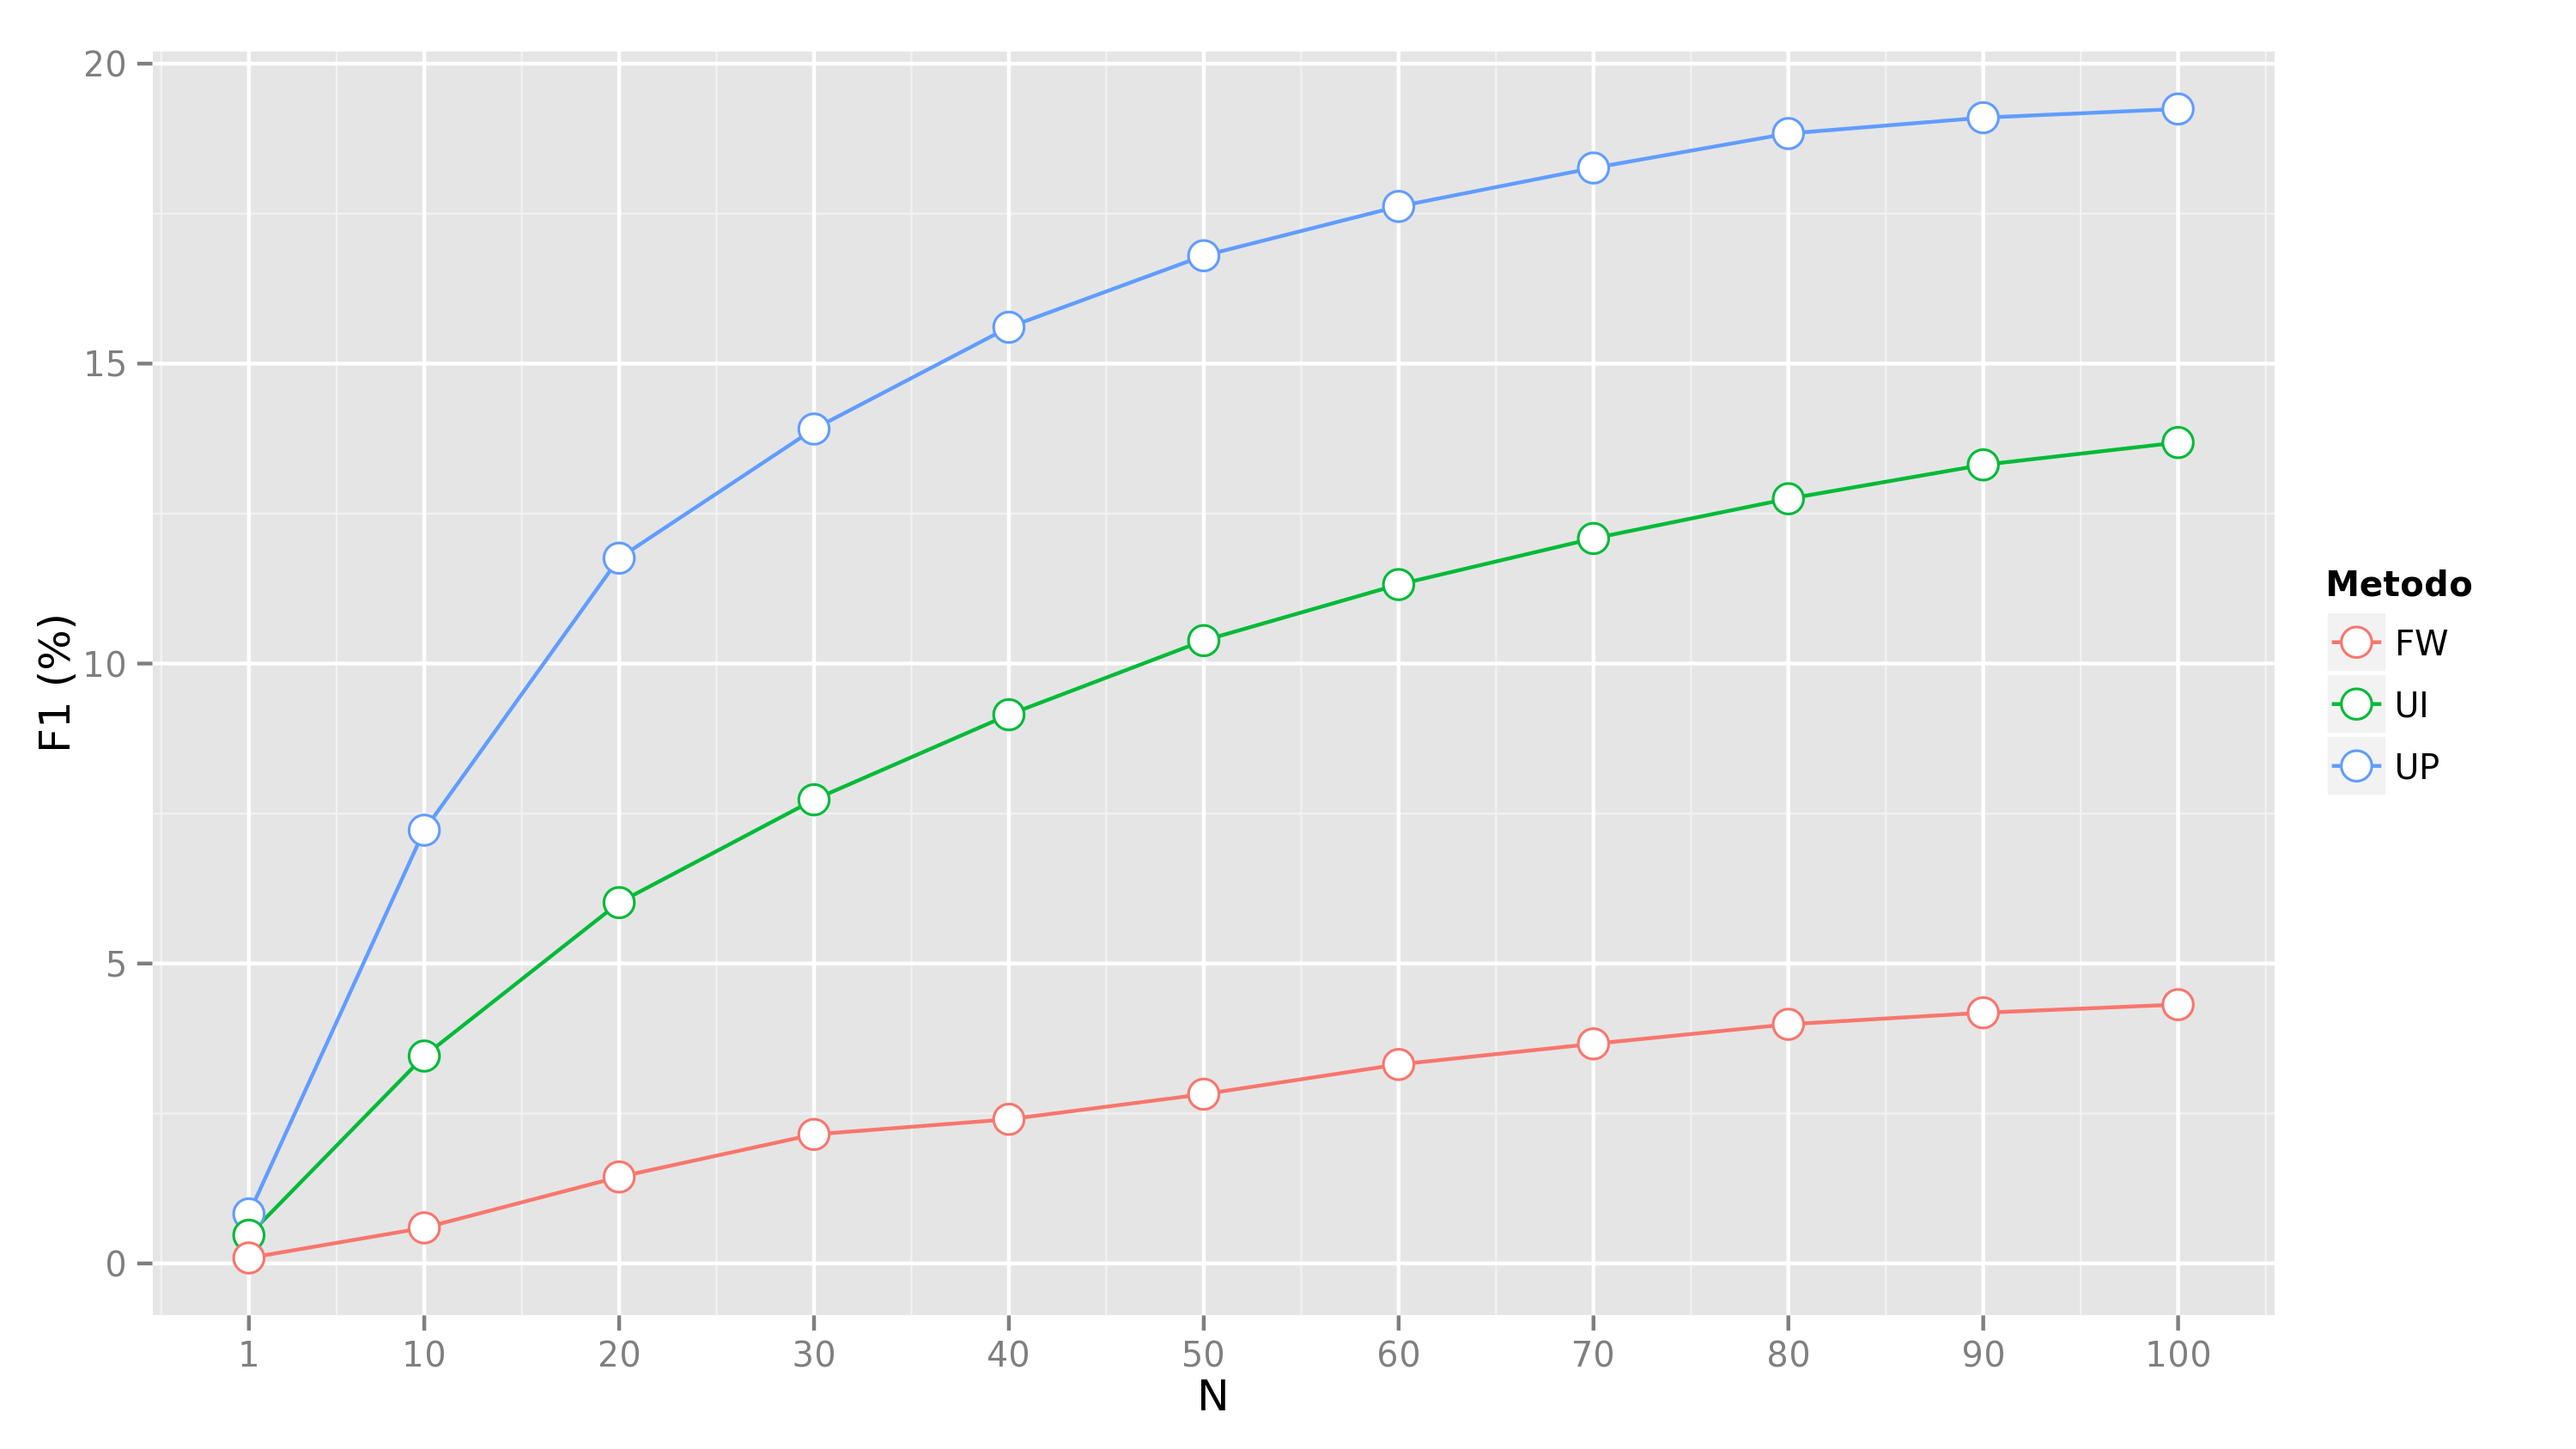
\includegraphics[width=.8\textwidth]{../img/F1_N_d}
    \end{center}
    \caption{$F_1$ $\times$ diferentes $d^f$}
    \label{fig:F1_N_d}
\end{figure}
\begin{center}
    Precisão e Abrangência diminuem com $d^f=J(A,B) ={{|A \cap B|}\over{|A \cup B|}}$
\end{center}
\end{frame}

\begin{frame}{Resultados}{Conjunto de atributos dos itens  $\mathcal{F}$}
\begin{figure}[ht]
    \begin{center}
    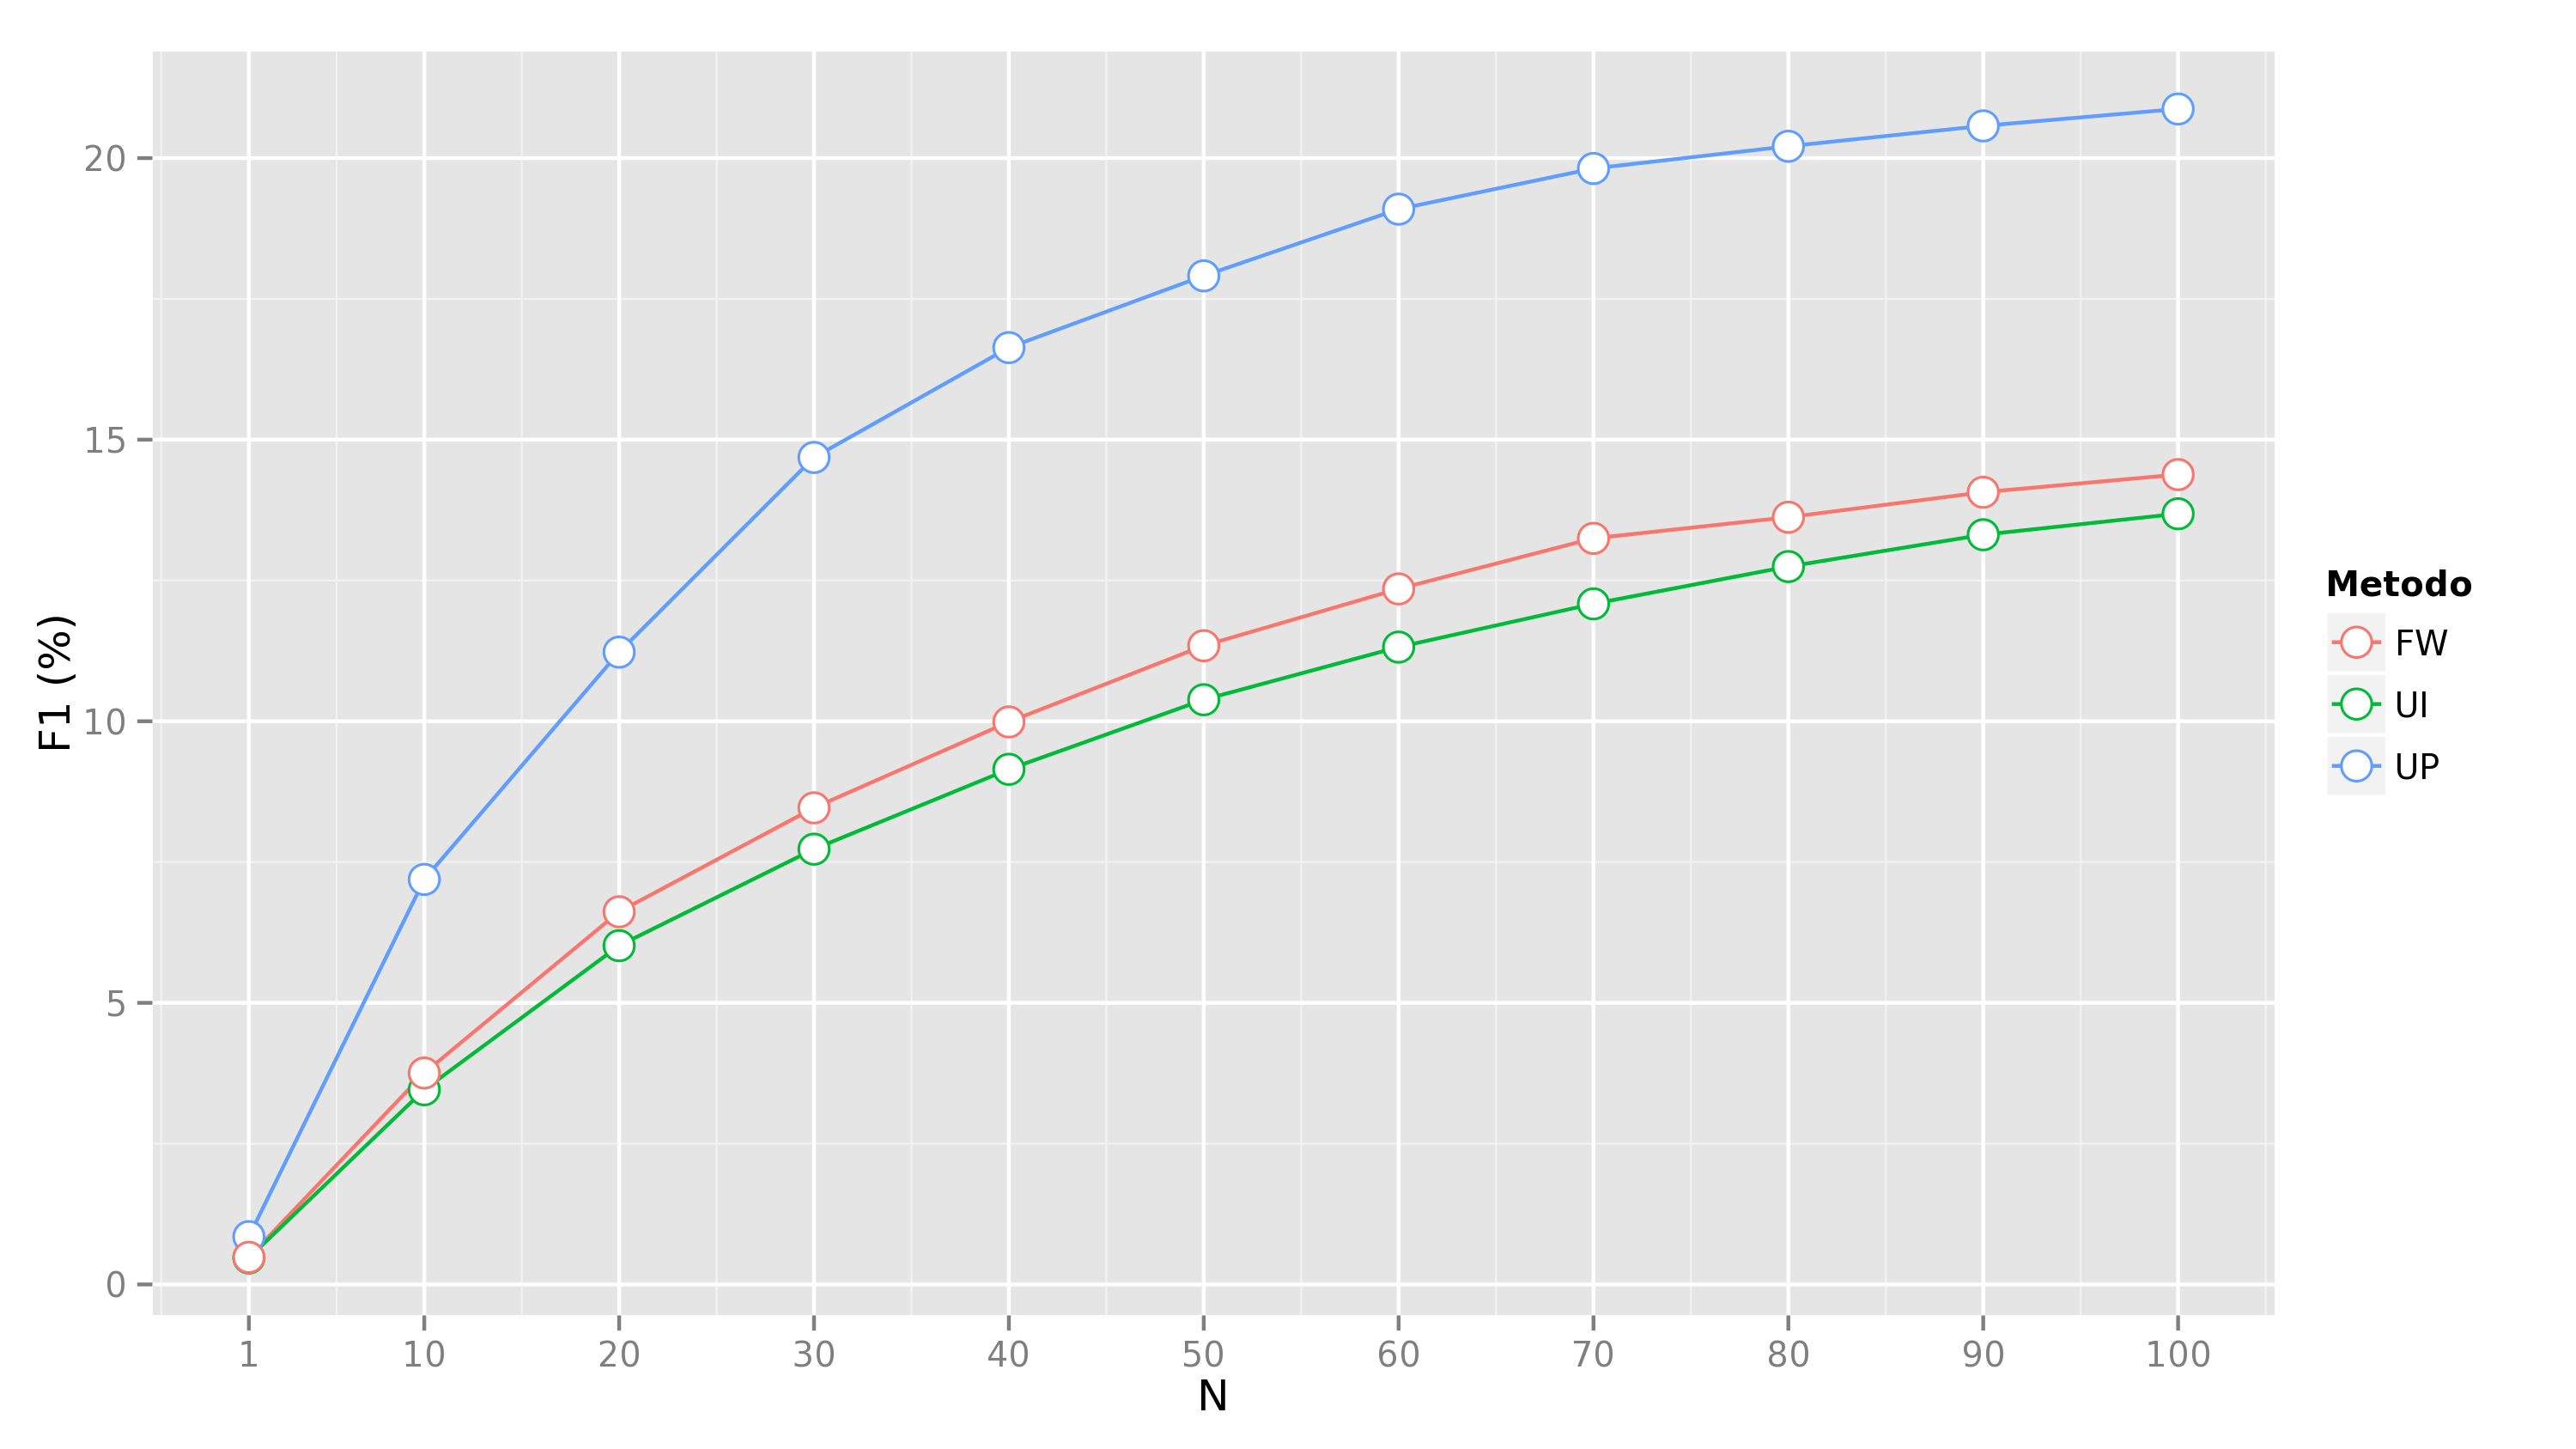
\includegraphics[width=.8\textwidth]{../img/F1_N_F}
    \end{center}
    \caption{$F_1$ $\times$ $\mathcal{F}$}
    \label{fig:F1_N_F}
\end{figure}
\begin{center}
    Precisão e Abrangência aumentam com remoção dos atributos \{data de lançamento, ano\}
\end{center}
\end{frame}




\begin{frame}{Resultados}{$M$, $k$, $W$}
\begin{columns}[b]
\column{.333\textwidth} %
\begin{figure}[ht]
    \begin{center}
    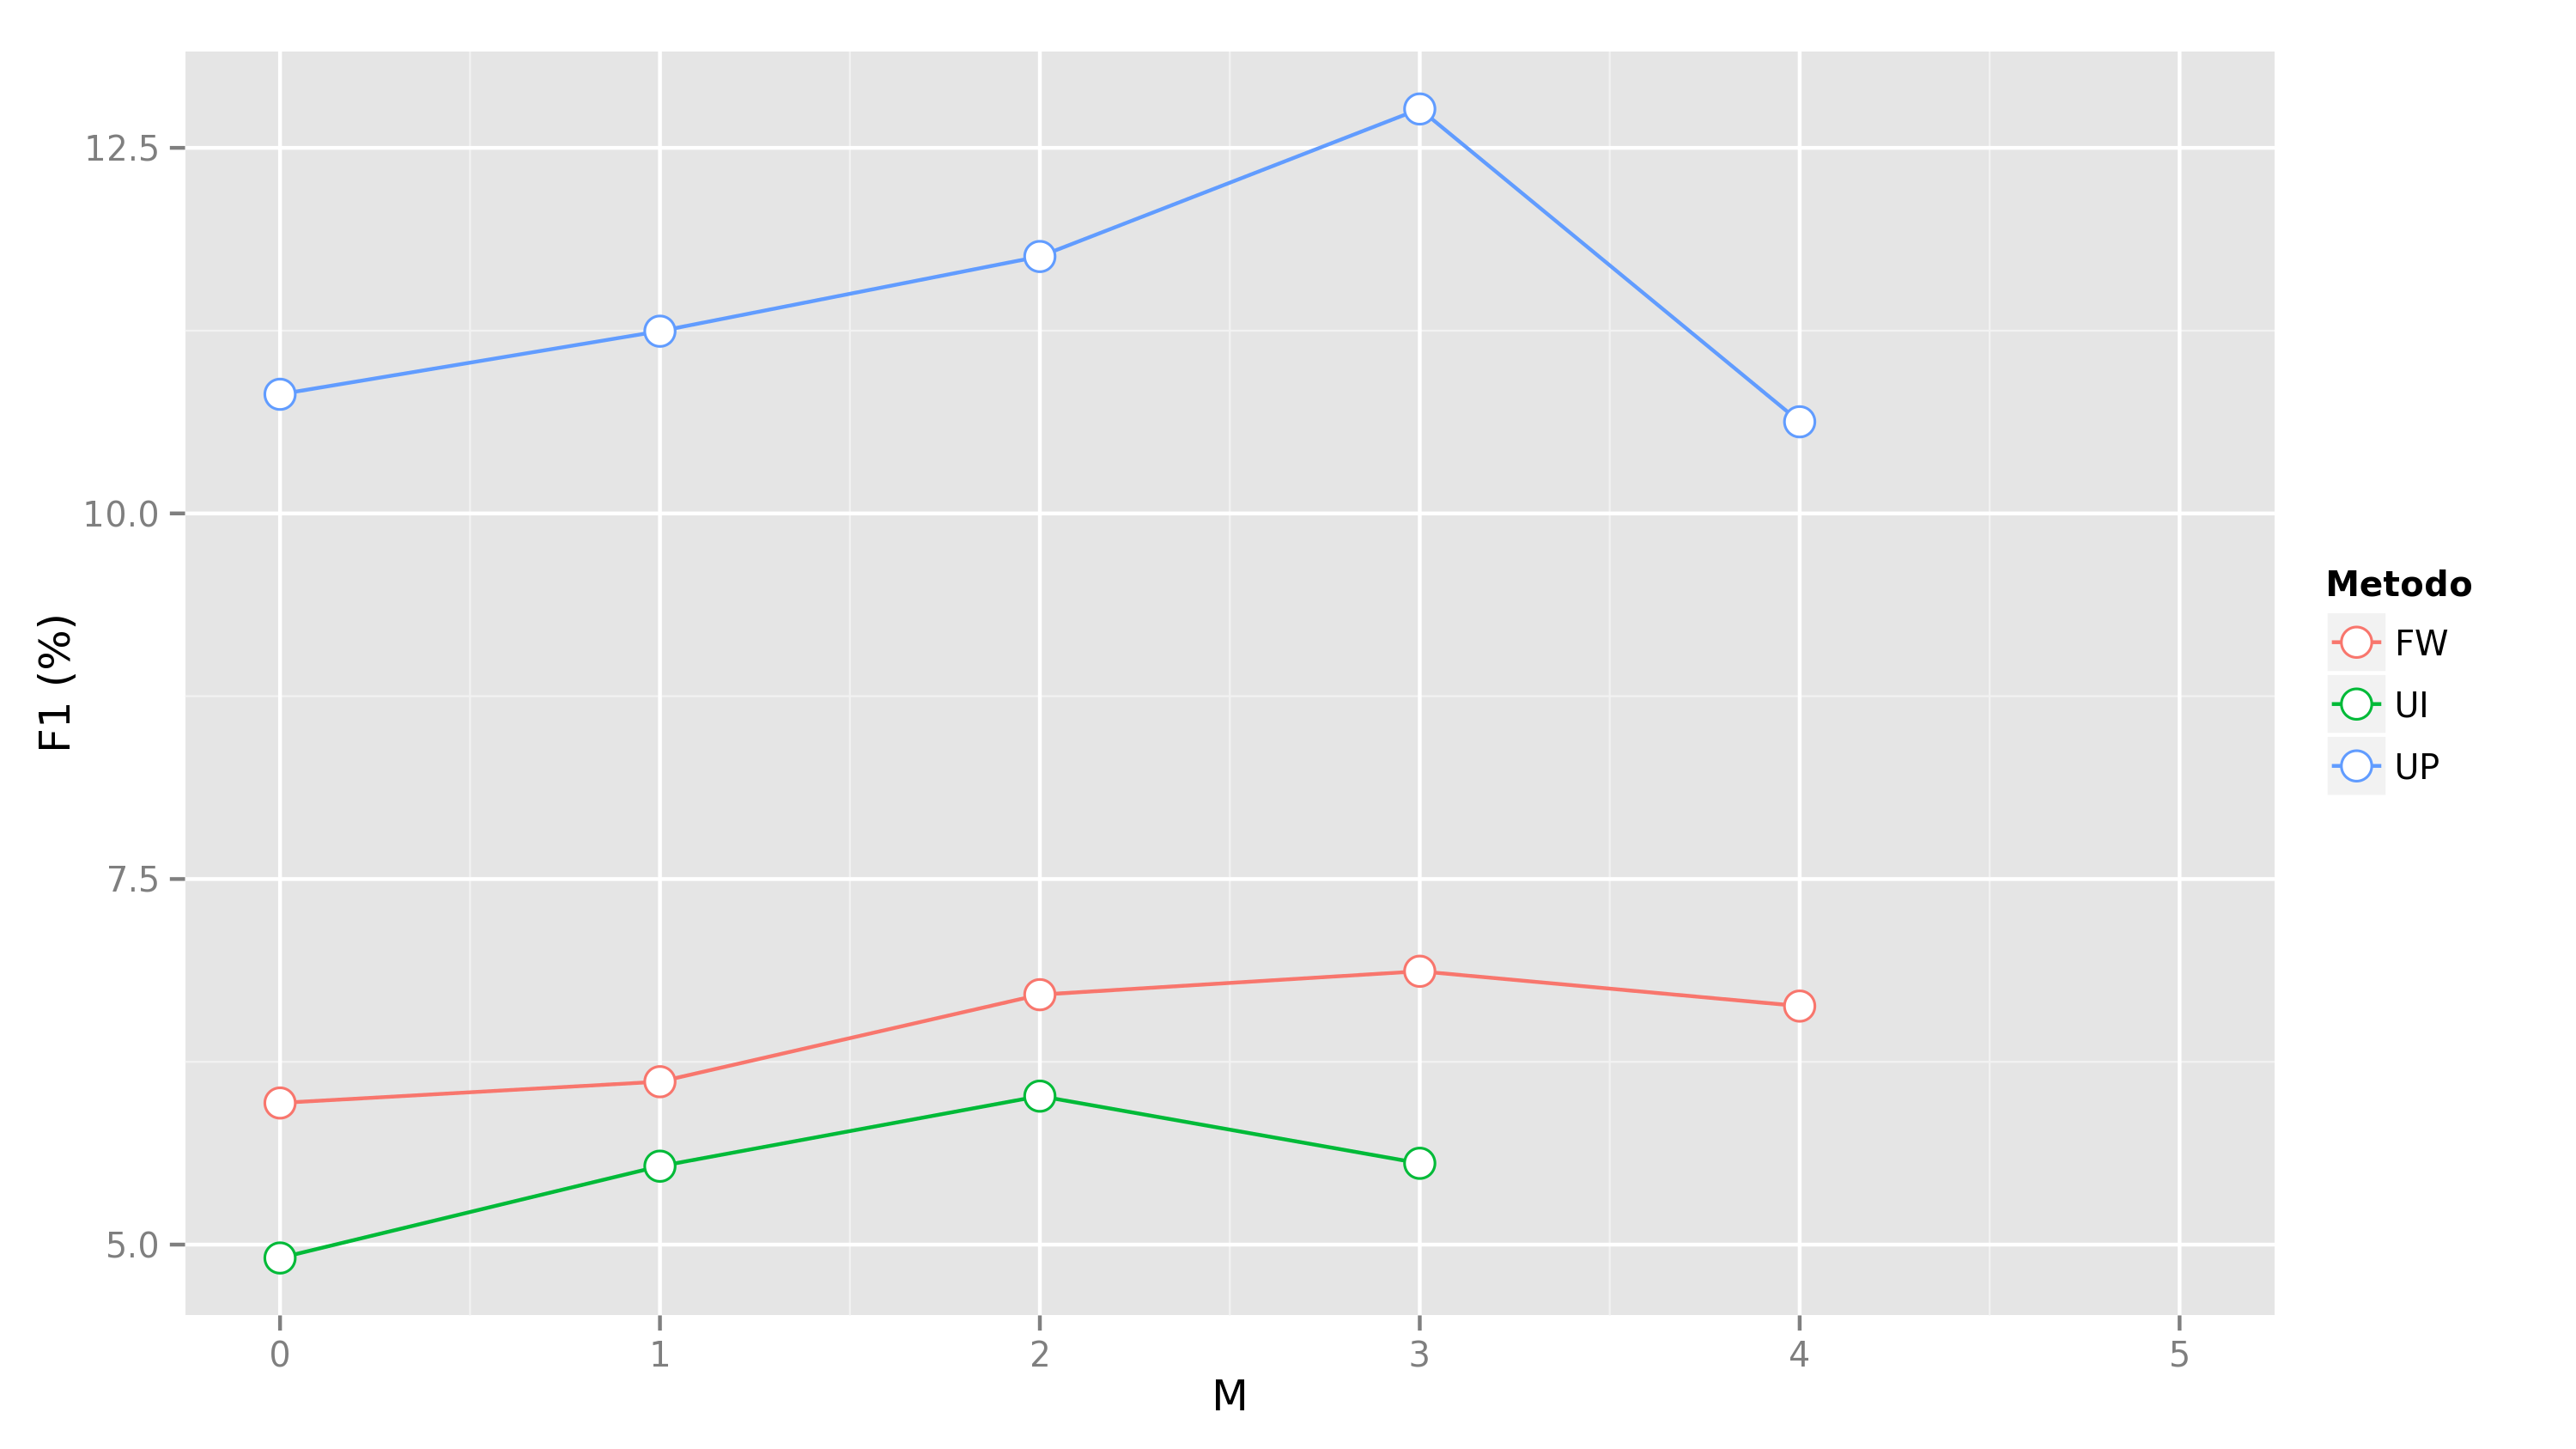
\includegraphics[width=1.1\textwidth]{../img/F1_M}
    \end{center}
    \caption{$F_1$ $\times$ $M$}
    \label{fig:F1_M}
\end{figure}

%Número de vizinhos mais próximos $k$
\column{.333\textwidth} % 
\begin{figure}[ht]
    \begin{center}
    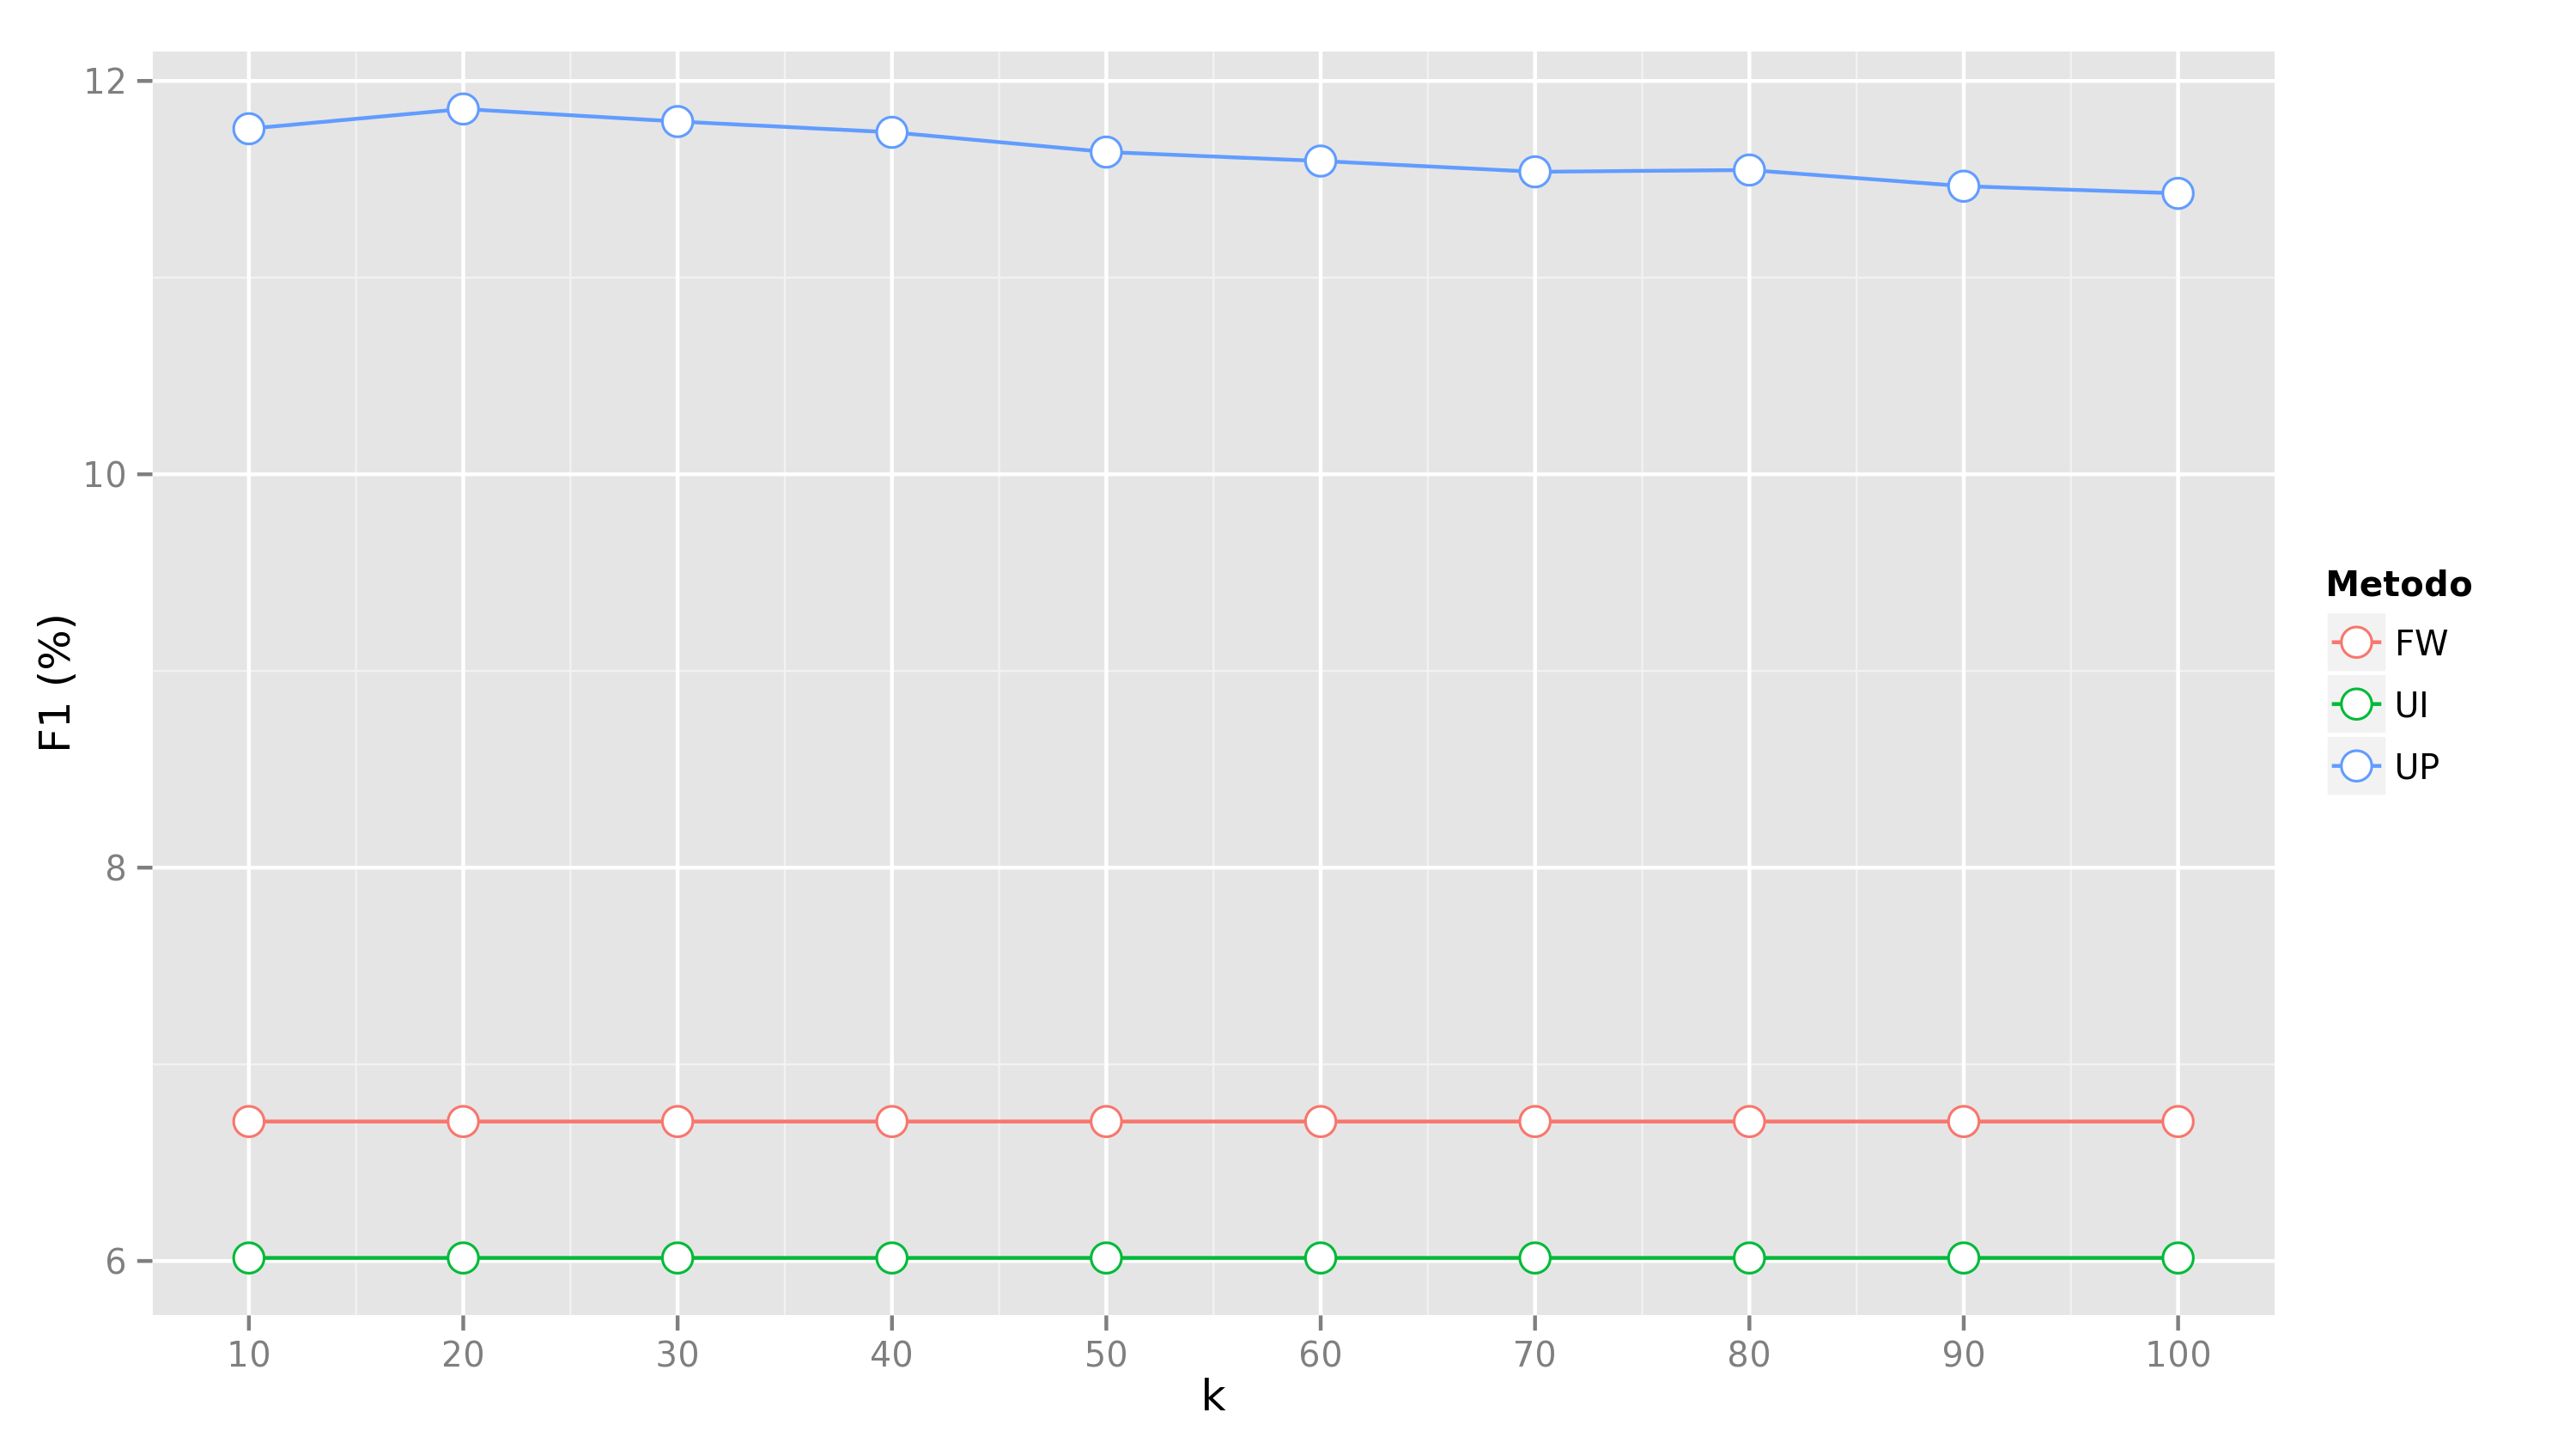
\includegraphics[width=1.1\textwidth]{../img/F1_k}
    \end{center}
    \caption{$F_1$ $\times$ $k$}
    \label{fig:F1_H}
\end{figure}
\column{.333\textwidth} % 

\begin{figure}[ht]
    \begin{center}
    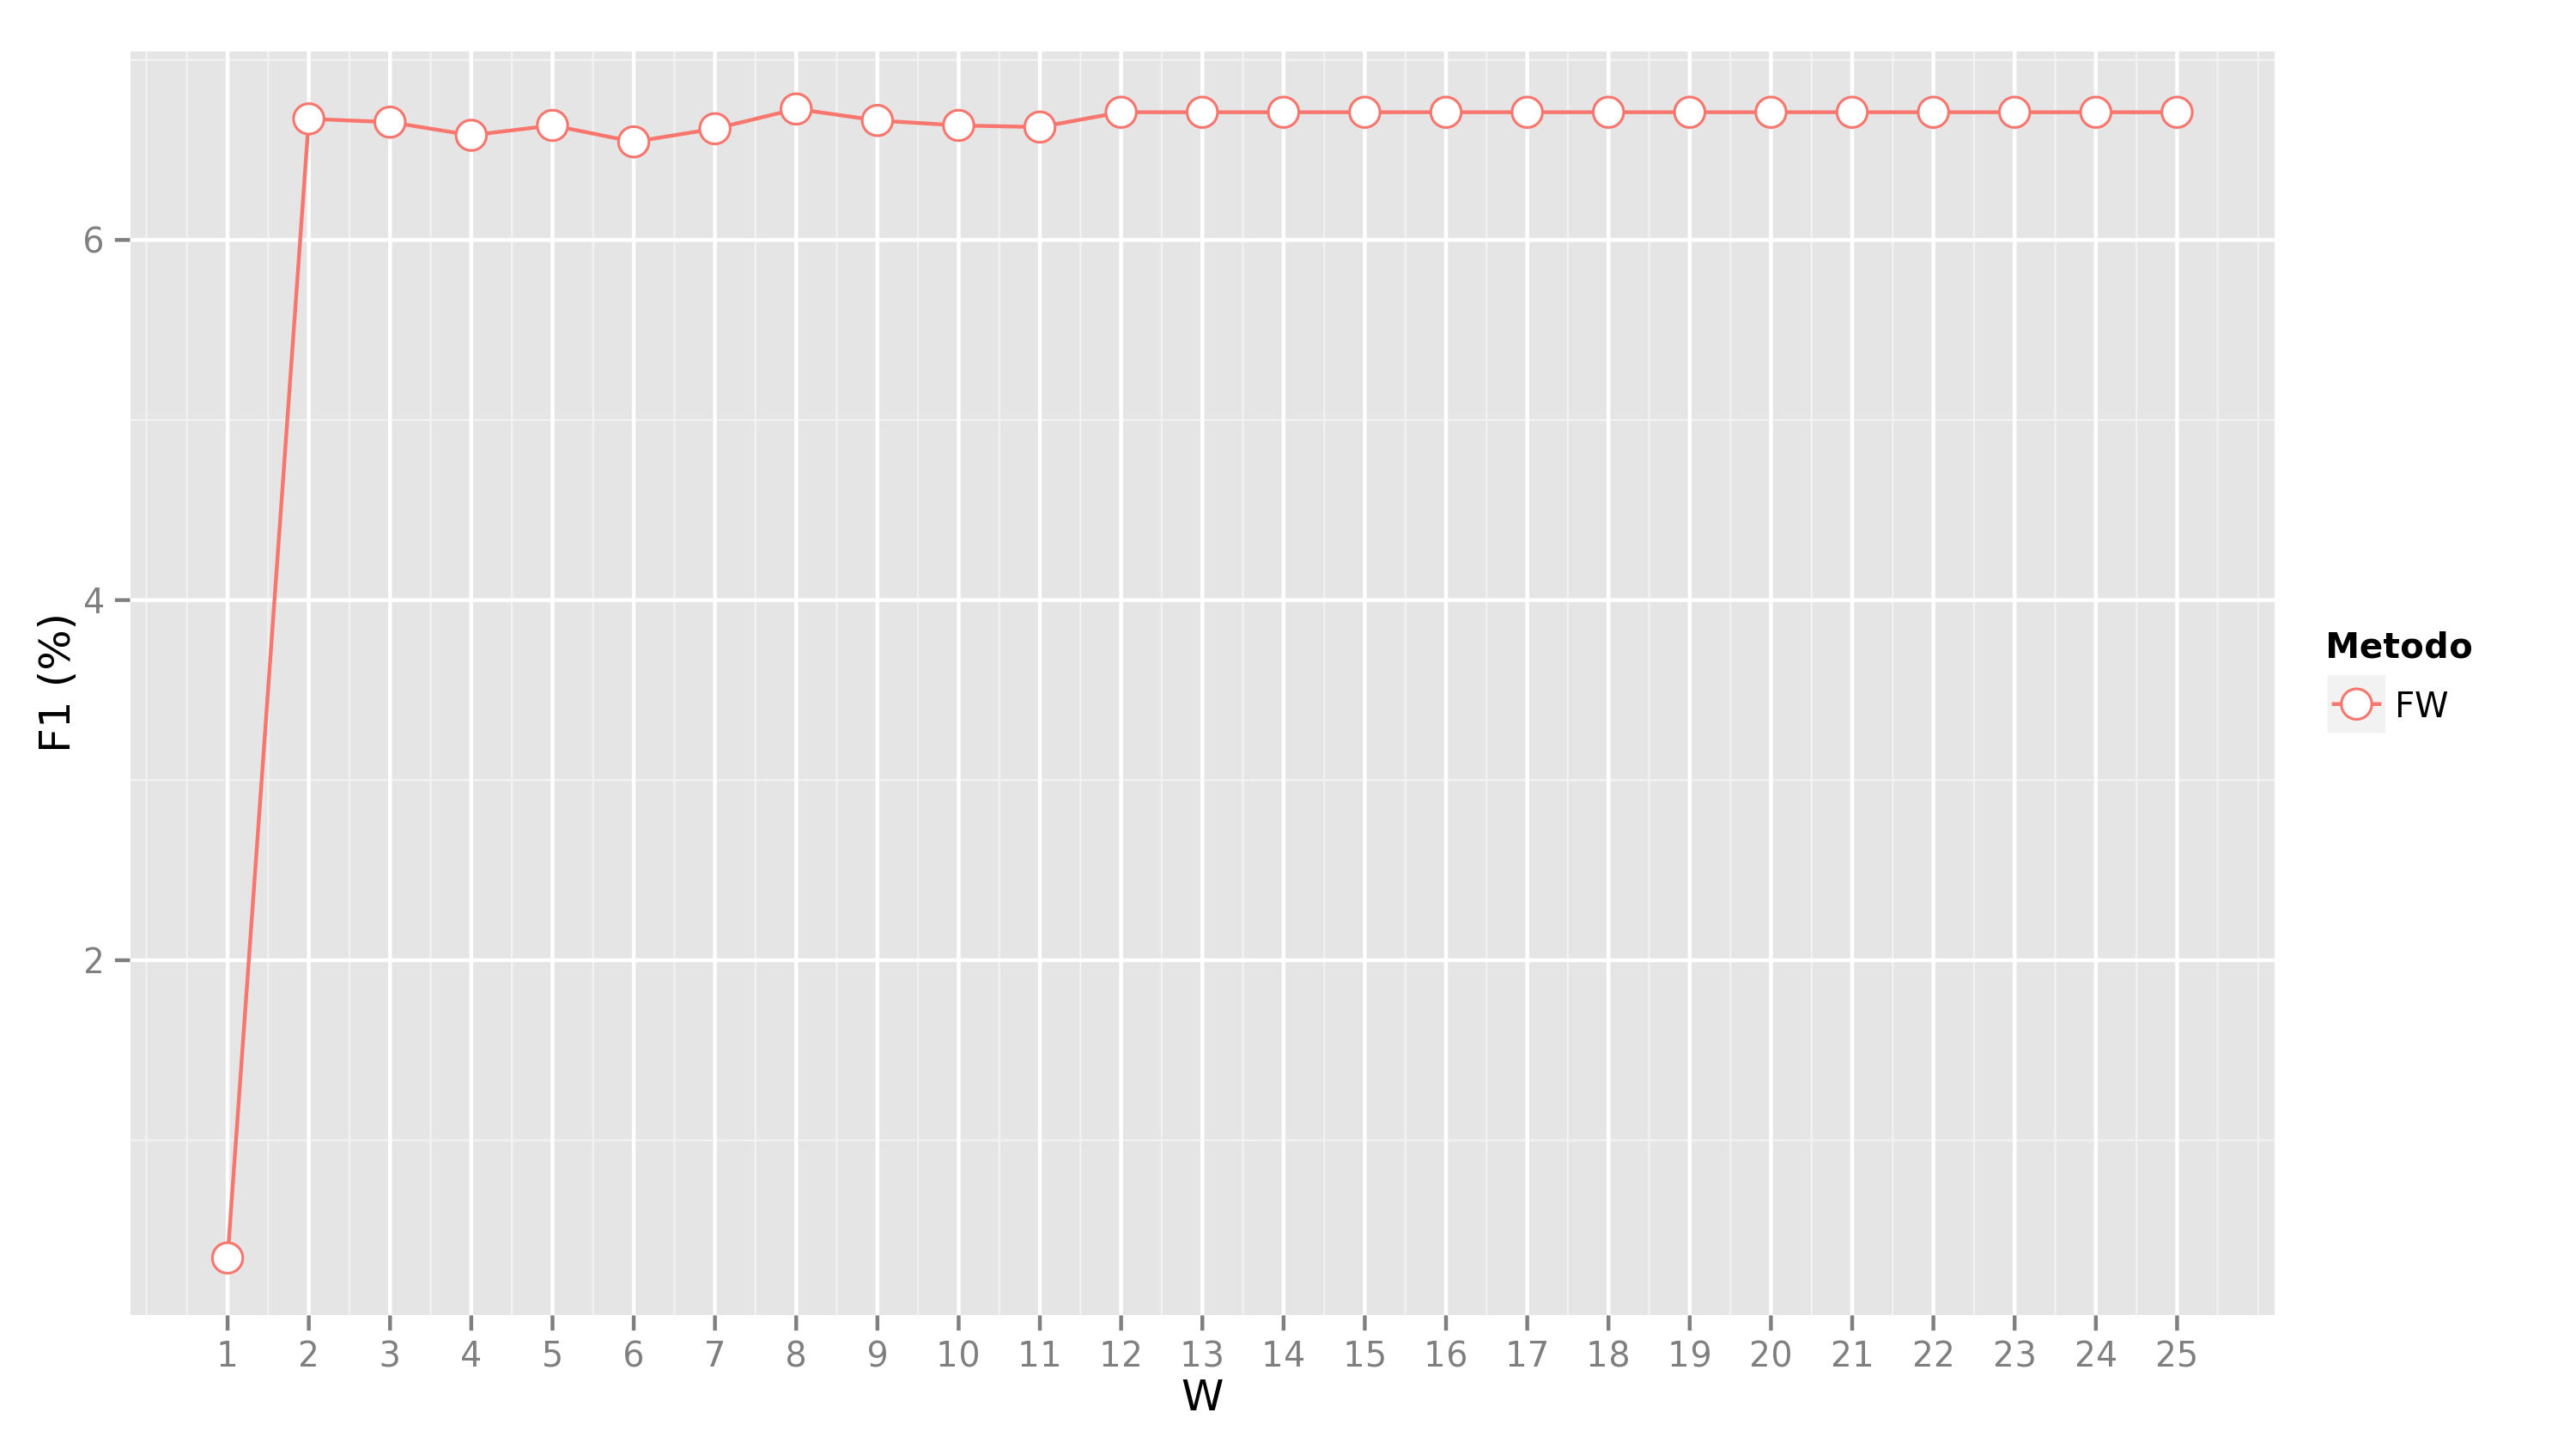
\includegraphics[width=1.1\textwidth]{../img/F1_W}
    \end{center}
    \caption{$F_1$ $\times$ $W$}
    \label{fig:F1_W}
\end{figure}
\end{columns}
\begin{center}
    Precisão e Abrangência praticamente constantes
\end{center}
\end{frame}



%\begin{figure}[ht]
%    \begin{center}
    %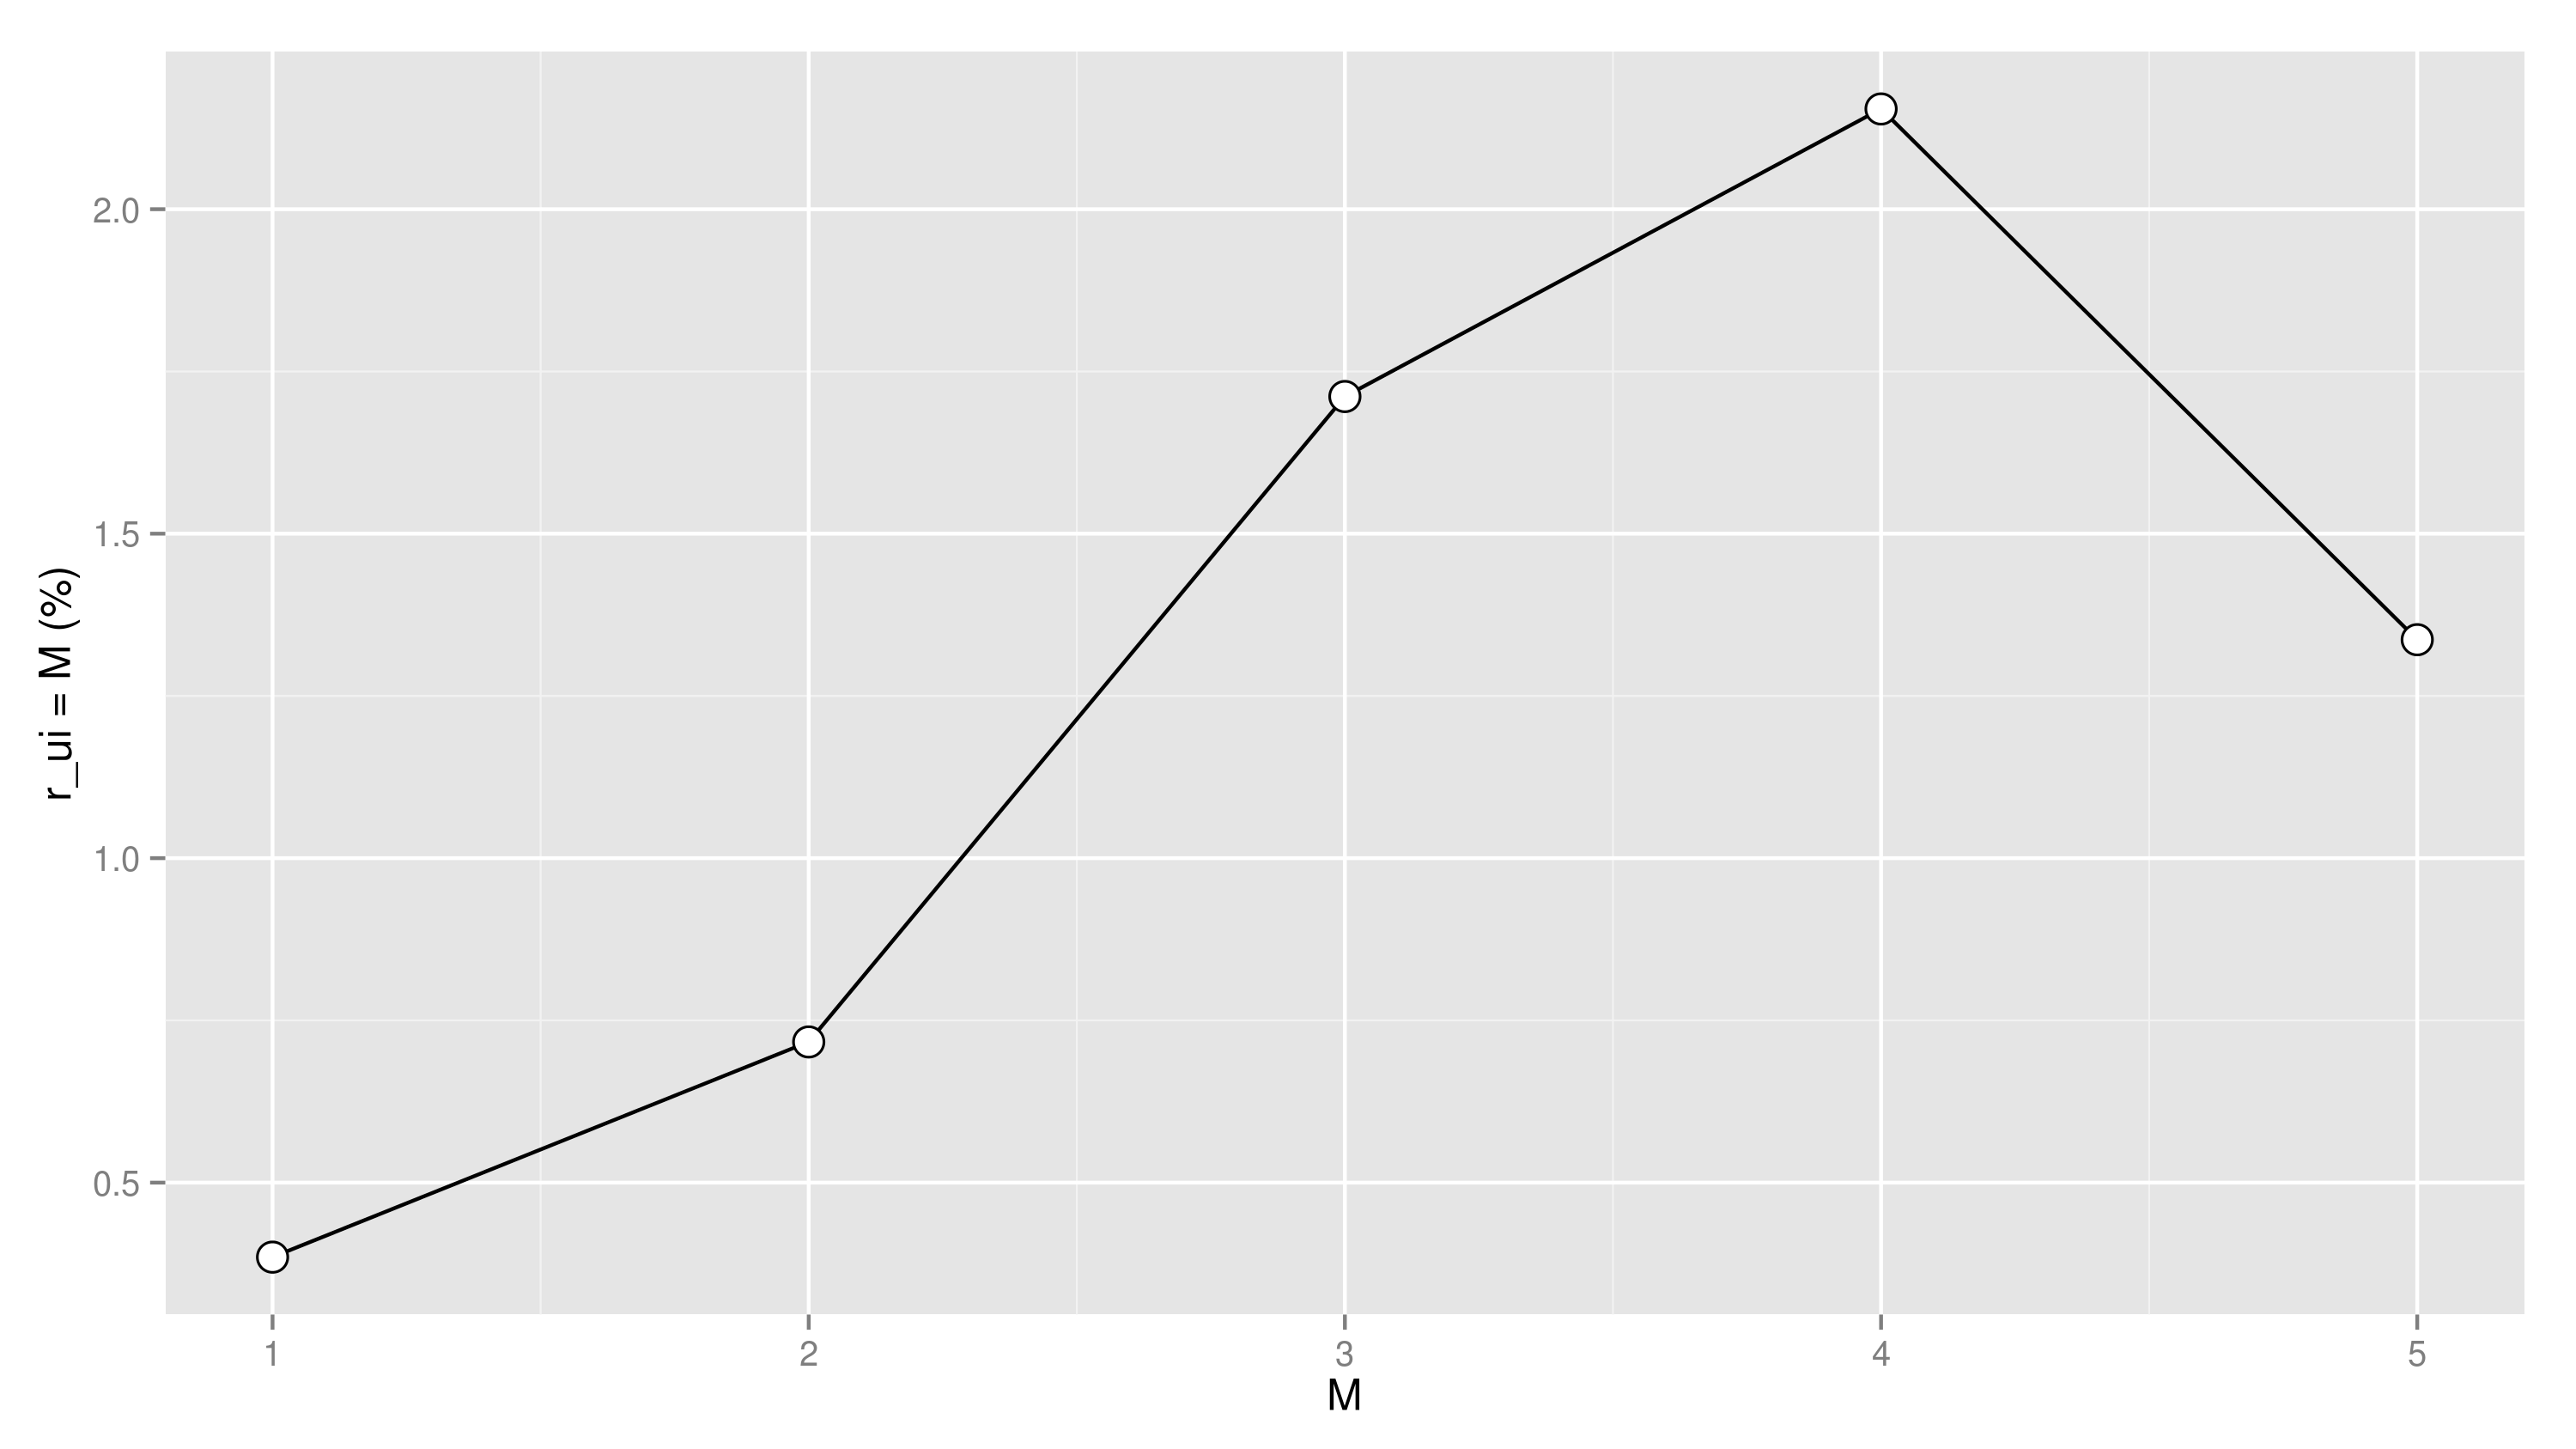
\includegraphics[width=1.1\textwidth]{../img/percentual_M}
%    \end{center}
%    \caption{\{\% $r_{ui} = M$\} $\times$ $M$}
%    \label{fig:percentual_M}
%\end{figure}

%!TEX root = index.tex
\section[Conclusão]{Conclusão}
\begin{frame}{Conclusão}
\textbf{Discussão}
\begin{itemize}
	\item Dependência entre qualidade de recomendação e $N$
	\item Mais avaliações $H$ é melhor que mais usuários $T$
	\item Muita influência de $d^f$, $\mathcal{F}$
	\item Pouca influência de $k$, $M$, $W$
\end{itemize}
\vspace{.5cm}
\textbf{Trabalhos futuros}
\begin{itemize}
	\item ``Sistema de Recomendação nas Nuvens''
	\item Eliminação de restrições de entrada/saída de dados
	\item Desenvolvimento de um \textit{driver} SQL 
	\item Reconstrução da biblioteca em C
	\item Aplicação em um banco de dados de um e-commerce real
\end{itemize}
\end{frame}
%%!TEX root = index.tex
\chapter[Cronograma]{Cronograma}
\label{chap:cronograma}

O cronograma de atividades da dupla busca seguir o cronograma proposto pela banca avaliadora dos trabalhos de conclusão de curso, estando sempre à frente das entregas em pelo menos uma semana. Dessa maneira, é possível apresentar a entrega antecipadamente ao orientador e falar sobre possíveis mudanças ou correções.

Além disso, semanalmente os alunos se reunem com o orientador a fim de conversar sobre o andamento do projeto, apresentar-lhe o esboço dos relatórios e discutir a implementação dos algoritmos. 

Para o segundo semestre, trabalharemos na implementação do sistema de recomendação já no período de férias escolares, para poder ter uma amostra funcional no início das aulas. Em seguida, daremos início ao relatório final em paralelo com os testes de performance do sistema de recomendação, e esperamos finalizar o projeto dentro do prazo estipulado.

O cronograma detalhado da dupla está descrito a seguir:

\begin{description}
	\item[09/07] Pré-tratamento do banco de dados
 	\item[16/07] Programação do método \textit{FW} e variantes, descritos no relatório final
 	\item[23/07] Programação do método \textit{UP} e variantes, descritos no relatório final
 	\item[30/07] Análise comparativa dos dois algoritmos
 	\item[13/08] Relatório de atividades de implementação
 	\item[27/08] Primeiros testes com o sistema (precisão e acurácia para uma base de testes)
 	\item[03/09] Testes com o sistema (validação cruzada)
 	\item[24/09] Melhorias incrementais e relatório de atividades
 	\item[15/10] Relatório aprofundado de atividades
 	\item[05/11] Elaboração da apresentação e finalização dos relatórios
 	\item[12/11] Melhorias incrementais
 \end{description} 
%\pagebreak
%%!TEX root = index.tex
\chapter[Andamento do Projeto]{Andamento do Projeto}
\label{chap:andamento_do_projeto}

%Tal relatório deverá conter 
%	descrição minuciosa 
%		do andamento do projeto
%		das etapas cumpridas, 
%		do planejamento do trabalho no segundo semestre, 
%		dos resultados alcançados  , 
%		das modificações em relação à proposta inicial, 
%	bem como uma avaliação precisa e detalhada 
%		dos resultados alcançados neste semestre , 
%		dos objetivos do próximo semestre 
%		da viabilidade de alcance do resultado programado  no fim do segundo semestre. 

Ao longo do semestre, o escopo deste Trabalho de Conclusão de Curso se alterou no que tange as possíveis soluções e aquilo que será entregue como produto.

De início, pensamos fazer um sistema de recomendação utilizando algoritmos de filtragem colaborativa baseada em itens, principalmente motivados pela leitura inicial de \cite{linden2003amazon}, que mostra as vantagens desse método comparado à filtragem colaborativa baseada em usuários. 

Todavia, percebemos que grande parte dos e-commerces estruturam seus bancos de dados em torno da descrição dos itens à venda e das informações dos clientes. As tabelas de itens podem possuir dezenas de atributos, dependendo do ramo de negócios da loja, tais como marca, esporte, categoria, cor, preço ou outros. Pouco detalhe é dado à interação entre esses dois grupos, visto que a tabela de histórico de compras se limita a informações como data e método de pagamento. Dessa forma supusemos que métodos de filtragem colaborativa, fundamentados na avaliação dos itens por parte dos usuários, teriam pior desempenho que métodos baseados em conteúdo, que exploram as características dos itens na recomendação. 

Ao considerarmos os possíveis algoritmos de recomendação, decidimos  não apenas testar um método de sugestão de produtos, mas sim fazer uma análise comparativa entre dois ou mais estratégias de recomendação. 

Os métodos do sistema de recomendação a ser desenvolvido serão, portanto, híbridos baseados em variantes de dois diferentes algoritmos, descritos nas Seções \ref{sec:algoritmo_baseado_na_pondera_o_de_atributos_} e \ref{sec:algoritmo_baseado_no_perfil_de_usu_rios_}, inspirados em \cite{symeonidis2007feature} e \cite{debnath2008feature}.

O primeiro artigo determina a similaridade de dois itens a partir de medidas de distância para cada um dos atributos dos itens, ponderadas por pesos determinados na regressão linear de uma equação descrita pelo interesse dos usuários em cada \textit{feature}. O segundo texto parte do princípio que os usuários estão interessados nos atributos dos itens, traçando correlações entre esses dois elementos até chegar nos pesos que servirão de base para o cálculo da similaridade inter-usuários, utilizada na recomendação pelo método da vizinhança (\textit{nearest neighbors}). Ambos estão descritos com maior detalhe no Capítulo \ref{chap:sintese_de_solucoes}.
%\pagebreak
\appendix
%%!TEX root = index.tex
\chapter{Documentação da biblioteca} % (fold)
\label{cha:documenta_o_da_biblioteca}

% chapter documenta_o_da_biblioteca (end)
\lstset{language=C}
\begin{lstlisting}[caption=\texttt{setup}.R]
read.history 
	input				filename, separator, header, col.names
	output			history
	description		Lê o arquivo de histórico de compras e retorna uma matriz correspondente. Os parametros separator e header indicam a formatação do arquivo e são opcionais. Caso header seja FALSE, col.names deve conter um arranjo de palavras indicando os nomes das colunas da matriz.

read.item
	input				filename, separator, header, col.names
	output			item
	description		Lê o arquivo de descrição dos itens e retorna uma matriz correspondente. Os parametros separator e header indicam a formatação do arquivo e são opcionais. Caso header seja FALSE, col.names deve conter um arranjo de palavras indicando os nomes das colunas da matriz.

read.user
	input				filename, separator, header, col.names
	output			user
	description		Lê o arquivo de descrição dos usuários e retorna uma matriz correspondente. Os parametros separator e header indicam a formatação do arquivo e são opcionais. Caso header seja FALSE, col.names deve conter um arranjo de palavras indicando os nomes das colunas da matriz.

get.r
	input				history
	output			r
	description		Le a matriz de histórico de compras e retorna a matriz de avaliação r_ui

get.a
	input				item
	output			a
	description		Le a matriz de descrição de itens e retorna a matriz de atributos dos itens a_if
\end{lstlisting}



\begin{lstlisting}[caption=\texttt{performance}.R]
hide.data
	input				r, Utrain.Utest, HIDDEN, random=FALSE, has.na=TRUE 
	output			matriz r com dados mascarados
	description		mascara os dados da matriz r para os usuários de teste da lista Utrain.Utest. HIDDEN é o percentual de avaliações a serem mascaradas. random é o modo de operação; caso seja TRUE, os dados são mascarados aleatoriamente para os usuários-teste. has.na indica se os itens não avaliados em r são indicados como NA ou como 0.

divide.train.test
	input				r, TRAIN
	output			lista contendo U.train e U.test
	description		divide os usuários em duas bases, uma de treinamento de uma de testes, segundo a proporção TRAIN

performance
	input				a, r, M=2, k=10, N=20, norm=TRUE, remove=FALSE, method, TRAIN=0.75, HIDDEN=0.75, W=FALSE, repick=FALSE
	output			lista contendo precisão, abrangência, medida F1 e tempo de execução do método
	description		norm indica se a matriz de avaliações deve ser normalizada. W, caso diferente de FALSE, indica a quantidade de pesos de atributos a serem utilizados no método FW
\end{lstlisting}

\begin{lstlisting}[caption=\texttt{fw}.R]
fw
	input				a, r, rtrain.rtest, Utrain.Utest, M, k, N, W
	output			iu
	description		Retorna uma lista de recomendação para todos os usuários Utest, após obter o modelo a partir dos usuários Utrain
\end{lstlisting}

\begin{lstlisting}[caption=\texttt{ui}.R]
ui
	input				a, r, rtrain.rtest, Utrain.Utest, M, k, N
	output			iu
	description		Retorna uma lista de recomendação para todos os usuários Utest, após obter o modelo a partir dos usuários Utrain
\end{lstlisting}

\begin{lstlisting}[caption=\texttt{up}.R]
up
	input				a, r, rtrain.rtest, Utrain.Utest, M, k, N
	output			iu
	description		Retorna uma lista de recomendação para todos os usuários Utest, após obter o modelo a partir dos usuários Utrain
\end{lstlisting}



\begin{lstlisting}[caption=\texttt{functions}.R]
b
	input				x, y
	output			1 se x > y ou 0 se x <= y
	description		A definição da função b_M é diferente da do artigo de referência, em que b_Pt(x) é  tal que x >= Pt

delta
	input				m, n
	output			1 se m == n ou 0 se m != n
	description		Delta de Kronecker

jaccard
	input				xs, ys
	output			número entre 0 e 1
	description		Índice Jaccard entre os conjuntos xs e ys	

h
	input				matrix, N=6
	output			imprime as primeiras N linhas e N colunas da matriz
	description		Caso a entrada seja um vetor, imprime os N primeiros elementos. 

top.N
	input				xs, N=10
	output			N maiores elementos da lista xs
	description		Usado na construção da lista de itens top-N 

index.top.N
	input				xs, N=10, ys.remove=NULL
	output			Índice dos N maiores elementos da lista xs
	description		ys.remove é uma lista em que se deseja excluir os elementos da lista top.N

normalize
	input				matrix, columns=FALSE
	output			matriz normalizada
	description		Caso columns seja TRUE, as colunas da são normalizadas dependendo do maior valor absoluto de cada uma delas
\end{lstlisting}
%\pagebreak
%%!TEX root = index.tex

% ----------------------------------------------------------
% ELEMENTOS PÓS-TEXTUAIS
% ----------------------------------------------------------
\postextual
% ----------------------------------------------------------

% ----------------------------------------------------------
% Referências bibliográficas
% ----------------------------------------------------------
\bibliography{bibliografia}
\end{document}
